% Dissertation
% 06/28/2013
% (Use \include{filename} in diss file

\documentclass[a4paper,12pt]{report} 	% report used for dissertations


\usepackage{anysize} 		% allows me to set margins
\usepackage{indentfirst}
\usepackage{apacite}		% for apa style
\usepackage{graphicx}		% for graphics
\usepackage{times}
\usepackage{mathtools}
\usepackage{textcomp }
\usepackage{amsmath}

\numberwithin{figure}{chapter}
\numberwithin{table}{chapter}
\numberwithin{equation}{chapter}

\marginsize{1.5in}{1.5in}{1.25in}{1.25in}	% left, right, top, bottom
\begin{document}
\linespread{2}					% double-spacing
\selectfont
\title{Evolving Synthesis Algorithms using a Measure of Timbre Sequence Similarity}
\author{Aron Glennon\\
  Steinhardt School of Education,\\
  New York University,\\
  New York,\\
  NY,\\
  10014\\
  \texttt{apg250@nyu.edu}}
\date{\today}
\maketitle
\linespread{1}
\selectfont
\begin{abstract}
The computer has provided composers with the ability to produce absolutely any sonic material within the human range of hearing. However, this power comes with a fundamental caveat: the composer must communicate to the computer what sonic material they are interested in generating, and this process is a non-trivial task. It is primarily the case that computer composition software is written to provide an interface to the composer that defines boundaries within which the composer may generate material; and while these interfaces have proven effective in producing a large variety of material, the paradigm of software developers providing specific boundaries for the composer to work within is not ideal and certainly not the only possibility. 

The motivation of this research is to explore a different paradigm, where the composer communicates to the software exactly what sort of timbal material it is interested in generating and the software produces an appropriate interface to help them realize that. It is based on the idea that the most natural way for the composer to communicate with a computer is via describing by example.

The proposed system accepts a short audio file with timbal content that the composer wishes to begin working with and, via an intelligent search algorithm, finds a synthesis algorithm able to produce like timbres, and constructs that algorithm within the Max visual programming environment for the composer to use. An appropriate intelligent search method and parameterization is proposed, which includes a definition of a timbre sequence similarity measure used to assess individual algorithms and steer the search path through synthesis algorithm space.

The definition of an appropriate timbre sequence similarity measures includes both a definition of an objective timbre space, wherein distance between points is semantically meaningful, and a definition of a suitable sequence similarity measure for discrete paths traced through this space.

This timbre sequence similarity measure is used to help steer a proposed intelligent search algorithm through synthesis space. The constituent parts of this algorithm are all varied, as are the input parameters to these parts, in order to find the optimal configuration for the problem domain.

Results are presented and discussed for all proposed pieces of this system, showing that such a system can be optimized to meet the stated goal of providing a computer music computer the ability to work with any desired sonic material provided a recording of similar material exists.

\end{abstract}

\renewcommand\abstractname{Acknowledgements}
\begin{abstract}

\end{abstract}


\linespread{2}					% double-spacing
\selectfont
\pagenumbering{roman}					

\tableofcontents
\listoffigures
\listoftables
	

\newlength{\QuarterPage}
\setlength{\QuarterPage}{1.0in}

\begin{flushleft}			% generates left-aligned paragraphs
\setlength{\parindent}{30pt}	% This starts every paragraph with an indent

				
\vspace*{\QuarterPage}
\newpage
\pagenumbering{arabic}
\chapter{Introduction} % * suppresses heading numbers	
Timbre has played an increasingly important role in composition since the beginning of the 20th century. With the advent of digital technology, composers have been given the power to generate sounds with boundless timbral variation. However, true timbral exploration is still out of reach for all but the the most technically inclined and dedicated, as the mechanisms that provide timbre control (synthesis algorithms) are often non-intuitive unless one has a strong understanding of the mathematics that underly their sound production; and even in this case, achieving a specific desired timbre often requires a large amount of trial-and-error. To further complicate things, a variety of synthesis algorithms exist, each suited to only produce a subset of all possible timbre. Therefore, in order to successfully generate a desired timbre (or explore a specific region of timbre space) one must first choose an appropriate synthesis algorithm and then find an appropriate parameter set for the chosen topology. Placing this burden on the composer requires them to spend more time on trial-and-error searching and less time composing. The less technically inclined the composer is, the more time they will likely spend performing tasks that are not beneficial to their compositional process. It is our goal to shorten this search process for all composers, which we hope will also remove the inherent bias towards the mathematically sophisticated.
	
Approaching timbre matching through the lens of automatic programming, we have developed a system intended to automate this search process by automatically generating a synthesis topology well suited to the desired timbre, while simultaneously finding an appropriate parameter set that realizes it. This system performs an intelligently directed search through all possible synthesis topologies and parameter sets in order to find a suitable algorithm to produce the desired timbre - supplied by the user.

We approached this research with the following goals:
\begin{enumerate}
\item To determine an appropriate environment to automatically generate synthesis topologies within and to establish an acceptable input-space representation for such topologies.
\item To decide upon a well-suited intelligent search algorithm for navigating the input space defined by subproblem 1 and to find the best architecture for that algorithm.
\item To find ways of restricting the search space and making the search algorithm more efficient and powerful without omitting optimal solutions.
\item To develop an objective timbre space in which distances are semantically meaningful, information regarding the temporal evolution of timbre is retained, and whose elements are invariant to changes in pitch and loudness.
\item To determine an appropriate similarity metric in the objective timbre space found in subproblem 4 that will be appropriate for comparing time-varying timbral content. This metric will help define an objective landscape over the synthesis algorithm input space whose global optimum will correspond to the desired solution.
\item To combine the solutions of the above subproblems into a system implementation capable of automatically generating synthesis algorithms that not only match the target timbre, but that also exhibit attractive properties for any synthesis algorithm.
\end{enumerate}

\section{Motivations}
This study attempts to develop a system that, given a desired location in timbre space, is able to construct a synthesis algorithm with a low-dimensional parameter set, low time-complexity, and low space-complexity that maps to that location. By intelligently choosing which algorithm and parameter mapping to use for a given region of timbre space, this system will act as a meta-synthesizer able to automatically construct efficient synthesis topologies for any timbral region.

This research has the potential to impact a number of areas of study including computer music, music information retrieval, artificial intelligence (of which automatic programming research is a subset), and signal processing.

Practically speaking, the proposed system will extend the sonic palette of any composer (or producer) utilizing digital audio effects or synthesis algorithms regularly in their works. The availability of a larger timbral tool set for composers will naturally lead to more experimentation and timbral exploration as composers will be able to create with timbre in ways previously not available to them. Placing the burden of timbral search on the computer would also free up more time to compose, likely leading to increased compositional output; a benefit to the music community as a whole.

In constructing this system, we investigate more appropriate ways of measuring local timbre similarity. Local timbre sequence similarity is a far less researched topic than global timbral similarity in the MIR community. However, we believe that much can be learned about timbre on a local time scale, especially in cases where its specific temporal evolution contributes greatly to its perception. Also, by investigating new objective timbre spaces whose distance measurements are semantically meaningful, this research will benefit MIR researchers interested in, for example, instrument classification, song similarity, audio fingerprinting, and vocalist recognition.

This study will also contribute to the growing body of research targeted toward the use of artificial intelligence in artistic applications. Most research in this area deals with the creation of artistic works by machines and there is much less work focused on using artificial intelligence to generate new tools for human creators interested in a more traditional creation process. This research hopes to change that trend by exemplifying the importance of tool generation for artists that are not satisfied with their present means of creation.

Specifically, within the domain of artificial intelligence, almost all practical automatic programming research targets designing software for solving scientific problems (e.g. robot mechanics, circuit board design). Therefore, this study, drawing primarily from the automatic programming research community, integrates a domain typically interested in solving scientific problems with one of artistic creation in a way not yet approached rigorously.

Therefore, this study is significant from both theoretical and practical perspectives and will contribute to a number of different disciplines ranging from applied computer science and digital signal processing to computer music composition, music production, and music information retrieval.

\section{Overview}
In this study, a system is developed to generate synthesis algorithms able to produce timbal content that is similar to that contained in a source audio file. The system proposed is based on a large body of research in timbre, timbre similarity, sequence similarity, and automatic programming. The necessary background, ideas developed around it, and exploration of these ideas is presented as follows:

Chapter 2 provides an overview of the prior work leveraged in this study. Beginning with a basic treatment of the complexities involved in defining `timbre', it moves on to enumerate the various kinds of sound synthesis algorithms in common use in computer music and discusses the difficulty of estimating appropriate parameters for a specific algorithm given a desired timbre. Various re-synthesis algorithms are presented as solutions to this problem, leading into a discussion of meta-synthesis and its advantages over re-synthesis. An overview of meta-synthesis research naturally extends to a discussion of artificially intelligent music systems in general, followed by a brief outline of those that specifically were developed to solve the meta-synthesis problem. Audio-implementation systems are covered next in the light of how they may inadvertently provide insight into how meta-synthesis techniques can be improved from their current primordial state. The chapter ends with a treatment of previous research in timbre similarity and how an appropriate timbre similarity measure is absolutely paramount to an effective meta-synthesis system and then an overview of genetic programming research, which is from where we source our intelligent search algorithm.

Chapter 3 starts with an overview of the proposed system design, discussing the complexities involved in setting up the intelligent search between two different processes written in different languages as well as how the system adapts the genetic programming paradigm to this problem domain. It then covers the design of the various experiments performed to optimize the various pieces of the search algorithm, providing a rational for the variations of each module involved in the experiments and the order in which the experiments are executed.

Chapter 4 presents the results of all experiments described in Chapter 3, provides conclusions based on these results, and suggests possible areas of future work.

\vspace*{\QuarterPage}
\chapter{Prior Work} % * suppresses heading numbers	
\section{Timbre}
While timbre is a term in common use within the music community, its precise definition has remained elusive. In his thesis on tracking timbre, Shiraishi notes this is in part because:

%\linespread{1}
\selectfont
\begin{quote}
The term `timbre' itself is often confused with two different distinctions. On one hand, we recognize that different acoustic instruments have timbre. The piano has timbre of the piano...for instance. On the other hand, one instrument can be played with a performer's delicate timbre manipulation' (2006, p. 4).
\end{quote}
%\linespread{1.7}
\selectfont
In other words, one can associate a single timbre to a single sound-producing body or to a single sonic ``character'' possibly produceable by many different sound-producing bodies. Nicol writes that `ecological listening states that humans are more likely to describe sounds with reference to the apparent source of that sound as opposed to certain characteristics of that sound' implying that the former association with timbre may be more often valid (2005, p. 23). However, for this research the latter association is more relevant and will be adopted going forward. 

Johnson and Gounaropoulos make a separate distinction between two different types of timbre that are also often confused, differing in time scale \cite{Johnson:2006pi}. They write, in their study on associating words with timbral features extracted from an audio signal, that ``by timbre we will mean the micro-level spectral characteristics of sound as discussed by Wishart, as opposed to the gross timbral distinctions used e.g. in the MPEG-7 standard'' (2006, p. 1). This refers to a confusion between local versus global timbral representations. We find the former of these two most relevant to this research and also adopt this going forward.

It is clear from the above examples that the many different interpretations of the word ``timbre'' make it a relatively opaque concept. Stowell and Plumbley note that ``evidence from perceptual studies tells us that timbre is multidimensional and probably non-linear'' (2008, p. 1). Otherwise, the results of this research often conflict, most likely due to the ambiguity associated with the term \cite[p. 4]{Fiebrink:os}, [p. 11]{Ciglar:2009uf}.

There are two approaches to defining timbre (see Figure 2.1): an additive definition and a subtractive one. Additive definitions explain timbre by associating it with things that it \emph{is}, while subtractive definitions attempt to explain timbre by defining what it \emph{is not}. The subtractive definition, most common in the literature, explains timbre as being the characteristics of a sound left over after removing pitch and loudness (Wessel, 1979, p. 45); (Toivianen et al., 1998, p. 225). Ciglar points out that this definition assumes that a sound has a definitive pitch in the first place, or equivalently, that unpitched sounds do not have timbre [p. 7]{Ciglar:2009uf}. A possible addendum to this definition may be that timbre is what is left after removing loudness and pitch, assuming a pitch even exists to be removed. However, such a definition is still unsatisfactory, and this is why a good deal of research has been carried out to define timbre using an additive definition.
\\
\begin{figure}[!htp]
\begin{center}
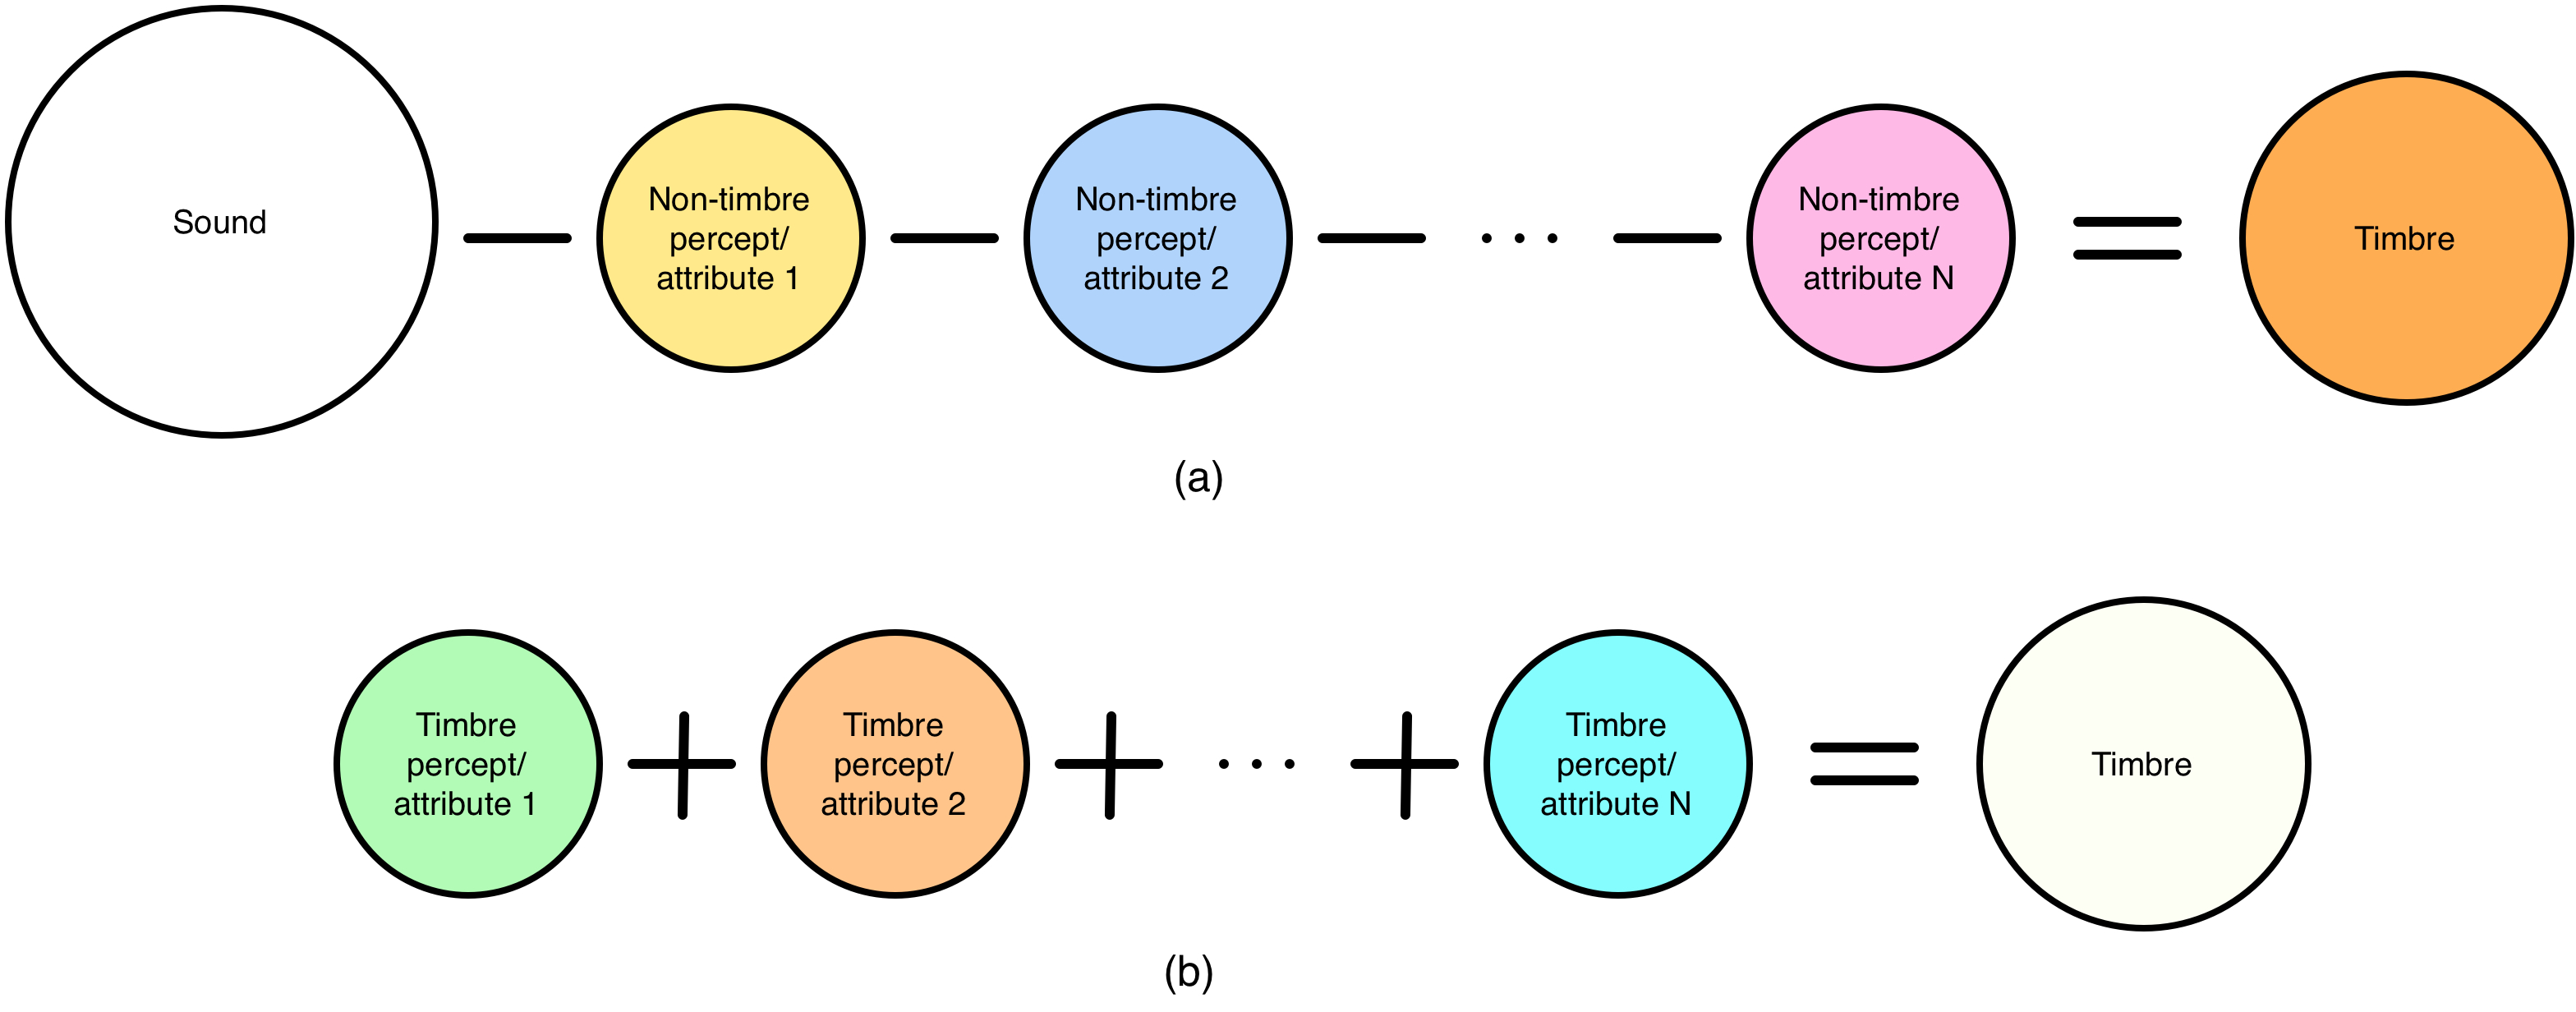
\includegraphics[scale=0.45]{SubtractiveVsAdditive}
\caption{Visual representations of (a) subtractive and (b) additive definitions of timbre.}
\end{center}
\end{figure}
In order to build an additive definition of timbre, one typically performs controlled perceptual similarity tests, uses the results to build a subjective timbre space where distances are semantically meaningful, and then associates the axes of this space with acoustic features \cite[p. 1]{Pampalk:2008xz}. Some of the earliest studies of subjective timbre spaces were performed separately by Grey and Wessel (Grey, 1975); (Wessel, 1979). Both use multidimensional scaling algorithms (MDS) to develop a timbre space from pairwise subjective similarity tests. MDS allows one to generate a space, typically two- or three-dimensional (though by no means limited to these), given a set of distance measurements between points, where the cumulative error in the distances provided between the points is minimized. In other words, MDS provides a way to generate a Euclidean space given a set of subjective measurements. However, in order to assign acoustic features to the axes resulting from MDS analysis on subjective measurements, one is left to find correlations between these axes with tested features. For example, using a two-dimensional timbre space, Wessel finds that the axes correlate with the spectral envelope and the nature of the onset transient (1979, p. 48). However, definitively assigning features to these axes based simply on correlation is misguided. As Caclin, McAdams, Smith, and Winsberg point out in their investigation into the properties of timbre, ``Given the multiplicity of acoustical parameters that could be proposed to explain perceptual dimensions, one can never be sure that the selected parameters do not merely covary with the true underlying parameters'' (2005, p. 2). 

Another problem with this approach is that MDS forces the user to choose the dimensionality of timbre space a priori, which will result in a feature set to explain timbre that may either contain too much or too little information.

Generating a perceptual timbre space using MDS also can be handicapped if not given a wide variety of timbral material that sufficiently covers the perceptual space. As Seago, Holland, and Mulholland note, if not using a wide enough variety of timbral material ``a sound in MDS space may have perceptually important features that no other sounds in the same space have---and, by the same token, two sounds could occupy the same location in a given MDS perceptual space, and nevertheless be audibly different'' (2008, p. 3).

Yet another drawback of subjective testing is discussed by Prandoni (1994). He notes that many of the pairwise similarity tests for timbre space construction are performed using common instrument sounds. Prandoni writes that this is a major problem in that ``the subjective ratings thus obtained are often affected by the listener's high-level notions of the structural features of the playing instruments rather than being a pure combination of sounds'' (1994, p. 2). He further points out that these studies find that features related to the attack and steady-state spectral envelope are often found to be highly correlated with the resultant timbre space axes because these are the features that ``remain constant among different nuances of color in recognizing an instrument'' (p. 8). Therefore, it is not clear whether other features beyond those that allow discrimination between instruments and instrument classes are perceptually relevant, but just not useful in the discrimination task. This is further complicated by the fact that one of the most often cited timbral features, the shape of the attack, assumes that for every ``timbre'' point there must be an attack. Nevertheless, acoustic features related to the spectral envelope and attack are the most widely used to generate objective timbre spaces for purposes of measuring timbre similarity.

From Prandoni's comments, one wonders if the features derived from these tests may best describe the intuition of timbre that is tied to the sound-producing body that created it, rather than that which relies solely on the sonic characteristics of the sound. This is supported by the fact that these tests ask a subject to note the similarity between whole instrument tones, rather than between attacks or steady-state portions separately. The result is that a single note played by an instrument will be placed as a single point in timbre space, rather than trace out a trajectory, which would seem more appropriate if the sonic characteristic of that note changes over its duration. In his treatment of both subjective and objective timbre spaces, Nicol writes that the single point vs trajectory delineation is one of the main differentiating characteristics between these two types of spaces (2005, p. 56). In an objective timbre space, each moment in time is represented by a point and as time evolves a trajectory is traced out through timbre space. This representation falls more in line with Johnson and Gounaropoulos' local timbre distinction \cite{Johnson:2006pi}. It also allows one to incorporate the temporal evolution of timbre into a similarity calculation as will be necessary when trying to find optimal matches to time-varying timbral content.
 
In this research, we are interested in such objective timbre spaces as our concept of timbre falls in line with the local timbre distinction and with that which represents the sonic character of the sound, regardless of the sound-production mechanism. Given this distinction, there is still ambiguity regarding ``whose'' percept of sonic character we refer to. For example, in a large auditorium the sound emanating from a violin will most certainly be perceived by the violinist as having a different character than that perceived by an audience member a hundred feet away due to the addition of reverberation. Since this research focuses on generating a system  that is able to understand the sonic characteristics of a given audio file, the \emph{who} can only be the computer, since no input will be given to the system regarding the acoustic space within which the audio file was recorded nor will it be given any information regarding the acoustic space within which the resultant synthesis algorithm will be used to generate sound. Thus, any reverberation or other distortions applied to a sound before it reaches a microphone for recording will be considered as part of the sonic characteristic of the desired sound, inseparable from the sound wave generated at the origin of the sound. Likewise, the computer will assume the synthesis algorithm it generates will be played in an aneachoic chamber in order to match the target sound.

\section{Sound Synthesis}
Timbre is a fundamental parameter of music, yet total and precise timbre control cannot be realized---or, at the very least, is severely limited---by acoustic means. Even the most skilled players are constrained by the physics of their instruments' sound production mechanisms (Wessel \& Wright, 2002, p. 11). However, with the advent of digital technology, the sound generator can be separated from its control interface and therefore no longer reliant on its physical properties (Malloch, Birnbaum, Sinyor, \& Wanderley, 2006, p. 1).  The resulting timbral freedom introduced by digital technology augmented the already increasingly important role timbre had taken in Western compositional practice starting from the turn of the twentieth century (Klingbeil, 2009, p. 1). In investigating the increasingly common compositional use of timbre, Nicola Bernardini and Jran Rudi (2001) write that by providing a �different, deeper and total control over timbre [computer music composition has placed a] stronger focus on the timbral aspects of composition -� on the micro-level.� (p. 3). This increased focus on timbre has spawned the design of numerous sound synthesis algorithms over the past fifty years in hopes to provide the composer with the level of control over timbre that they have enjoyed for years with pitch and loudness.

The different approaches used in designing synthesis algorithms have varied widely throughout the history of sound synthesis. A number of sources provide surveys of the most popular techniques (Roads, 1996); (Miranda, 1998); (Cook, 2002). Miller Puckette's \emph{The Theory and Technique of Electronic Music} (2007) stands out among the rest in that he not only describes the underlying mathematics behind a number of different synthesis algorithms, but he also provides the user with a blueprint for design and timbral exploration. This book in combination with Puckette's earlier paper, \emph{Combining Event and Signal Processing in the MAX Graphical Programming Environment} (1991), provides a comprehensive look into designing synthesis algorithms using a graphical programming environment. The intent of these writings is not to compare and contrast the efficacy of the algorithms presented, but instead only to illustrate their inner workings. However, when a composer is ready to select a specific synthesis algorithm to work with, the results of such comparisons are paramount to the decision-making process. In order to assess the strengths and weaknesses of each algorithm, one must have a clear understanding of the desirable properties of a timbre producer/manipulator.

These properties have been discussed by a number of respected figures in the field of computer music at various levels of depth (Smith, 1991); (Jaffe, 1995); (Wessel \& Wright, 2002). Smith's treatment is relatively superficial in large part because these properties are not his paper's main focus. Jaffe's list of properties presume that a synth's main purpose is to mimic a real-world sound producing body, which is not always necessarily the case. Wessel and Wright mix the desirable properties of synthesis algorithms with those of control interfaces, often blurring the lines between the two within the same listed property. Most recently, in his treatment of composing with timbre, Nicol (2005, p. 40) provides four desirable properties for an ideal synthesizer: ``fast synthesis'' (i.e. computational efficiency); a ``wide timbral range'' (i.e. the ability to produce any desirable timbre); ``easy parameterization'' (i.e. an intuitive, low-dimensional mapping between parameters and sound); and ``low data requirements'' (i.e. low memory storage requirements). In other words, Nicol believes that an ideal synthesizer will provide the composer with an intuitive, low-dimensional parameter set that they may use to achieve (and manipulate) any desired timbre. Additionally, the underlying synthesis algorithm will ideally work in real-time and use a small amount of memory.

One of the most comprehensive comparative studies of synthesis algorithms is presented by Tolonen, V\aa lim\aa ki, and Karjalainen (1998). In this report, the authors categorize each synthesis algorithm under evaluation into one of four groups: abstract algorithms; sampling and processed recordings; spectral methods; and physical models (as originally proposed in (Smith, 1991)). Among the many algorithms treated, Tolonen et al. choose the most popular (also known as ``classical'' synthesis algorithms) to evaluate, and find that variants within each category perform similarly to their classical counterpart in regards to the proposed criteria (1998, p. 101). The classical synthesis methods investigated in their study were sampling synthesis (sampling and processed recordings), additive synthesis (spectral methods), FM synthesis (abstract algorithms), and digital waveguide synthesis (physical models). A more complete list of algorithms can be found in Table 2.1.
\\
\begin{table}[h!]
\begin{center}
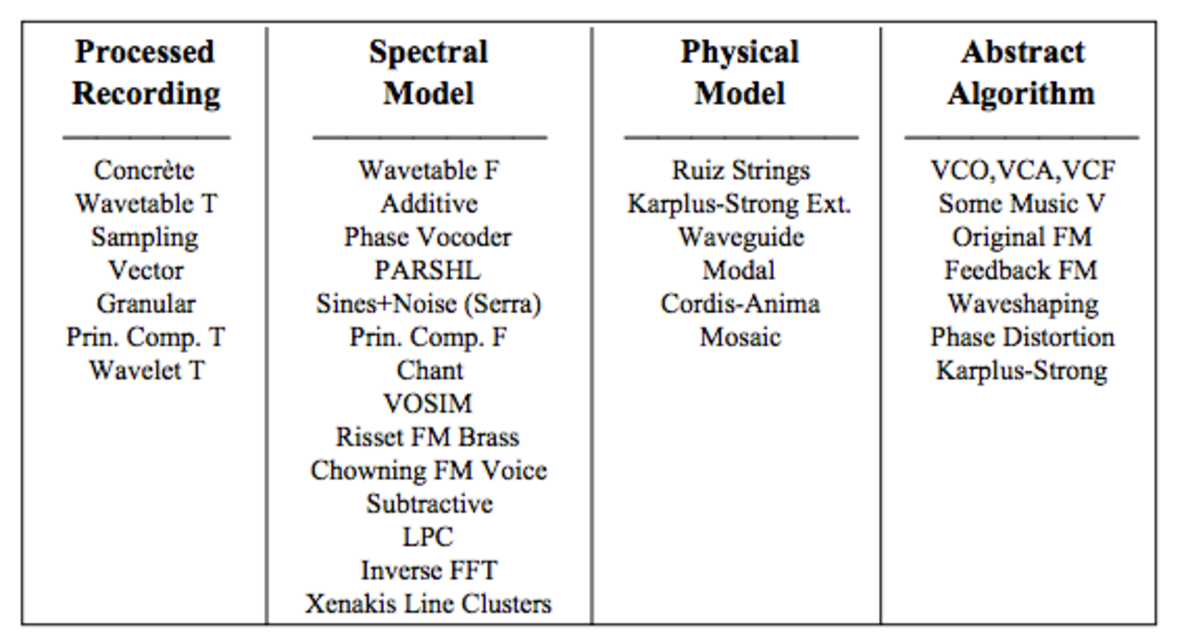
\includegraphics[scale=0.7]{SynthesisTechniqueTaxonomy}
\caption{Synthesis Technique Taxonomy (Smith, 1991)}
\end{center}
\end{table}
Sampling synthesis (see Figure 2.2) ``is a method in which recordings of relatively short sounds are played back'' (Tolonen et al., 1998, p.10). Using sampling, one can turn any audio recording into a musical instrument by simply assigning the playback of the recording to a switch (Heise, Hlatky, \& Loviscach, 2009, p.1). This type of synthesis dates back to the 1920's and certainly became prominent in 1950 when Pierre Schaeffer founded the Studio de Musique Concrete in Paris (Tolonen et al., 1998, p. 3). Like all sampling and processed recordings methods, sampling synthesis� flexibility is dependent on the size of the database containing the pre-recorded audio segments. Thus, to obtain a truly flexible sampling synthesizer ``the required amount of memory storage is huge'' (Tolonen et al., 1998, p. 11). As the flexibility of the system grows and one has enough material to generate small variations in timbre, doing so becomes more difficult as the number of samples to choose from during any single discrete movement in timbre space becomes unwieldy. Thus, while sampling synthesis is computationally efficient and requires a low-dimensional parameter set, there is a fundamental tradeoff between its ability to generate a wide variety of timbral material and the amount of memory it requires. It is also nontrivial to transform a given timbre in a smooth way, which, in his more recent survey of synthesis techniques, Smith writes is the true ``fundamental problem with sampling synthesis'' (2006, p. 22).
\\
\begin{figure}[h!]
\begin{center}
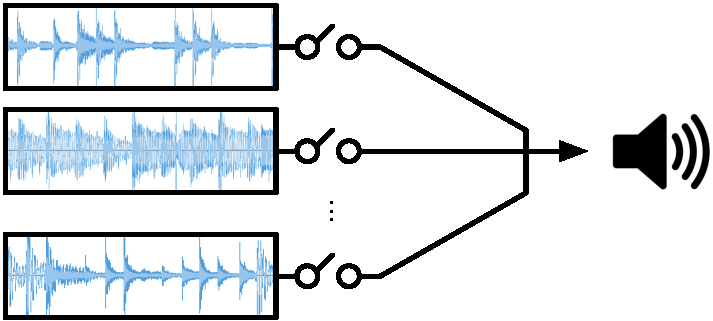
\includegraphics[scale=0.8]{SamplingSynthesis}
\caption{Sampling Synthesis}
\end{center}
\end{figure}
Granular synthesis (see Figure 2.3) `is a set of techniques that share a common paradigm of representing sound signals by ``sound atoms'' or grains...the synthetic sound signal is composed by adding these elementary units in the time domain' (Tolonen, V\aa lim\aa ki, \& Karjalainen, 1998, p.13). In his dissertation on analysis/synthesis techniques (which we be covered later), Klingbeil adds that 'granular synthesis may be viewed as a particular specialization of sampling synthesis...[It] offers the possibility to decouple the time and frequency evolution of a sound, as well as impart particular characteristics modulating between rough, smooth, or stochastic textures' (2009, p. 6). Thus, unlike sampling synthesis, granular synthesis allows one to transform smoothly between timbres. However, this comes at the price of a higher dimensional parameter space, forcing the user to specify `the shape of the overall ``cloud'', the fundamental frequency, the way in which the individual grains are generated, the structure of the individual grains used, etc' \cite[p. 5]{Johnson:1998sh}. In Nicol's dissertation investigating mappings between synthesis parameter spaces and timbre spaces, he notes that the non-intuitive mapping between this high dimensional parameter space and timbre space makes `emulation of target timbres a non-trivial process' (Nicol, 2005, p. 49). Granular synthesis requires less memory than sampling synthesis, but is also less efficient (although real-time algorithms do exist). Vercoe, Gardner, and Scheirer point out that granular synthesis is `best suited to the generation of noisy or textural sounds like water, wind, applause, and fire' (1998, p. 6).
\\
\begin{figure}[h!]
\begin{center}
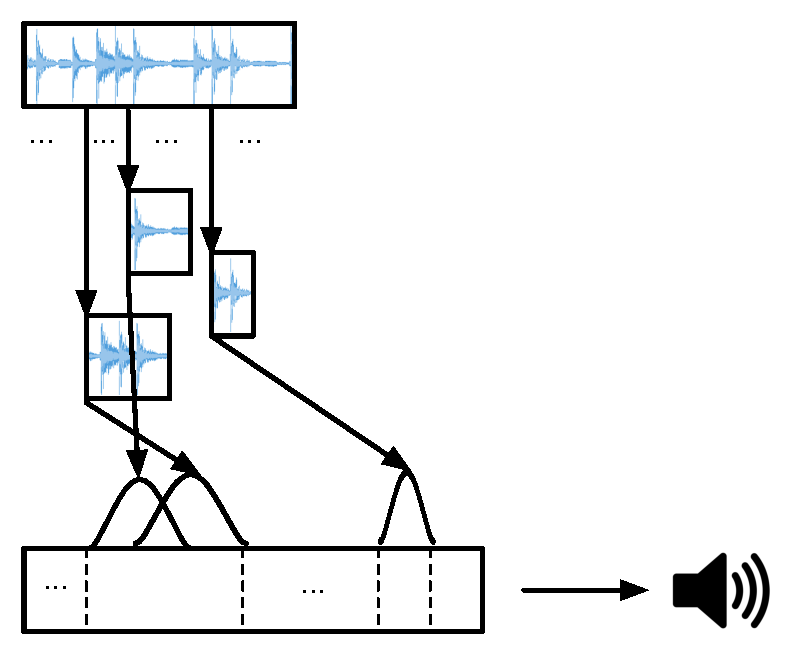
\includegraphics[scale=0.8]{GranularSynthesis}
\caption{Granular Synthesis}
\end{center}
\end{figure}
Additive synthesis (see Figure 2.4) ``is a method in which a composite waveform is formed by summing sinusoidal components to produce a sound'' (Tolonen et al., 1998, p. 17). Based on Fourier analysis, ``additive synthesis can in theory synthesize arbitrary sounds if an unlimited number of oscillators is available'' (Tolonen et al., 1998, p. 94). However, as the numbers of oscillators increase, so does the number of controllable parameters and, therefore, what adding oscillators gains in flexibility, it loses in controllability (Klingbeil, 2009, p. 7). It is because of this that additive synthesis is best utilized for generating harmonic or quasi-harmonic signals where little noise is present (Vercoe et al., 1998, p. 5). Additive synthesis also requires a number of parameters to be changed simultaneously in order to move a small distance in timbre space, which is unattractive. The desirable properties that additive synthesis satisfies are low storage (although the control data can require a lot of memory) and the ability to generate, in theory, any timbre, but its parameter space is high-dimensional and therefore difficult to control.
\\
\begin{figure}[h!]
\begin{center}
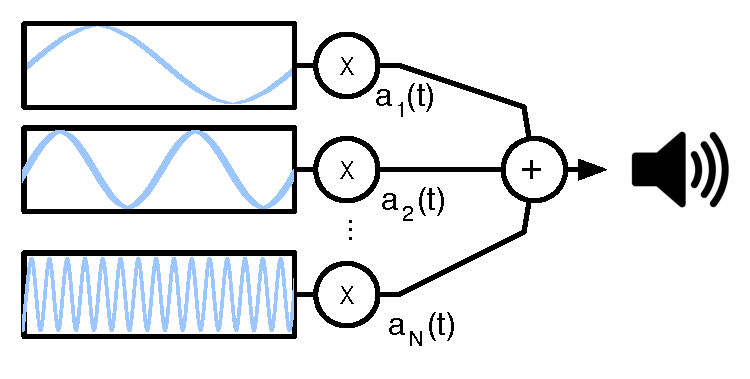
\includegraphics[scale=0.8]{AdditiveSynthesis}
\caption{Additive Synthesis}
\end{center}
\end{figure}
Subtractive synthesis (see Figure 2.5) is similarly based on Fourier analysis, but works by subtracting sinusoids from a spectrally rich source to generate material rather than building up material by adding sinusoids together, as in additive synthesis. The `subtraction' is performed by a time-varying filter whose coefficients are supplied by the user. In order to achieve complex and temporally evolving sounds, the parameter space can grow to the size of additive synthesis and therefore will suffer from the same controllability issues (Tolonen, V\aa lim\aa ki, \& Karjalainen, 1998, p. 48). If one uses a simple network of filters to try to reduce the size of the parameter space, `the resulting tones have a distinctive ``analog synthesizer'' character that, while sometimes desirable, is difficult to avoid' (Vercoe, Gardner, \& Scheirer, 1998, p. 5). Thus, one must trade timbral flexibility with the controllability of the algorithm. Similar to additive synthesis, the control data can require a lot of memory during sound production. Also, the efficiency of the algorithm and the facility to move around timbre space varies with the complexity of the time-varying filter or network of filters.
\\
\begin{figure}[h!]
\begin{center}
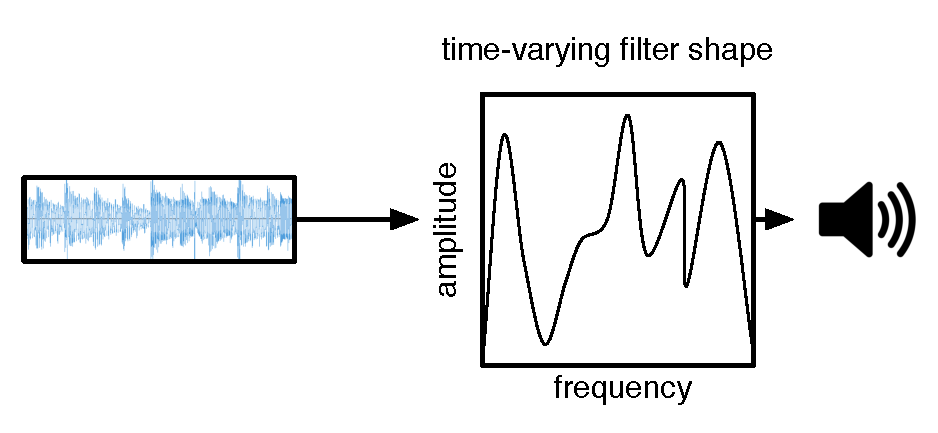
\includegraphics[scale=0.8]{SubtractiveSynthesis}
\caption{Subtractive Synthesis}
\end{center}
\end{figure}
FM synthesis (see Figure 2.6), in its most basic form, contains two oscillators, which are connected so that one oscillator�s waveform modulates the frequency of the other. There are only a few parameters with which to generate a large range of timbral material, which is desirable, but due to an inherent nonlinear mapping between parameter space and control space, ``FM has become widely regarded as a difficult synthesis type to control'' (Mitchell \& Creasey, 2007). This is for two reasons. First, the nonlinearity provides a non-intuitive relationship between a given set of parameters and the sound it produces (Nicol, 2005, p. 45). Second, a  nonlinear mapping means that small changes in the input parameters can map to large changes in the timbre and thus fine timbral manipulation can be difficult (Jaffe, 1995, p. 2). Another undesirable quality of FM synthesis is that the characteristic FM sound is ``fairly metallic, so the FM output is often filtered in order to produce a more natural sound'' (Nicol, 2005, p. 45). The benefits of FM synthesis are that is ``is very cheap to implement, uses little memory, and [as previously mentioned] the control stream is sparse'' (Tolonen et al., 1998, p. 92).
\\
\begin{figure}[h!]
\begin{center}
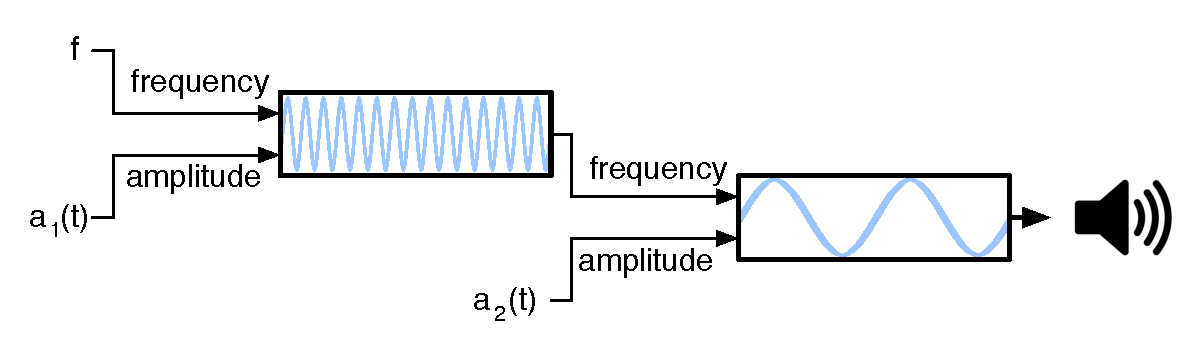
\includegraphics[scale=0.65]{FMSynthesis}
\caption{FM Synthesis}
\end{center}
\end{figure}
Digital waveguides (see Figure 2.7) are ``based on a general solution of the wave equation in a one-dimensional homogeneous medium'' (Tolonen et al., 1998, p. 63). They are basic linear time-invariant (LTI) structures that allow one to develop physical models of various instruments. Their parameters are intuitive and small in number, aiding in timbral manipulation. However, specific waveguide networks are designed to imitate a single sound producing body and therefore are timbrally restricted in comparison to additive synthesis. Also, as Smith (1992) comments in his seminal paper on digital waveguides, ``new models must be developed for each new kind of instrument, and for many instruments, no sufficiently concise algorithm is known'' (p. 86). In fact, as Tolonen et al. point out, any sound producing object that requires a two- or three-dimensional waveguide mesh to represent its governing physics will be computationally expensive to model and, therefore, only simple physical models based on waveguides will be able to run in real-time (1998, p. 99-100). Thus, digital waveguides provide a low-dimensional, intuitive parameter set and low storage requirements, but can be computationally expensive for complex sounds and require separate topologies for each region of timbre space (Nicol, 2005, p. 50).
\\
\begin{figure}[h!]
\begin{center}
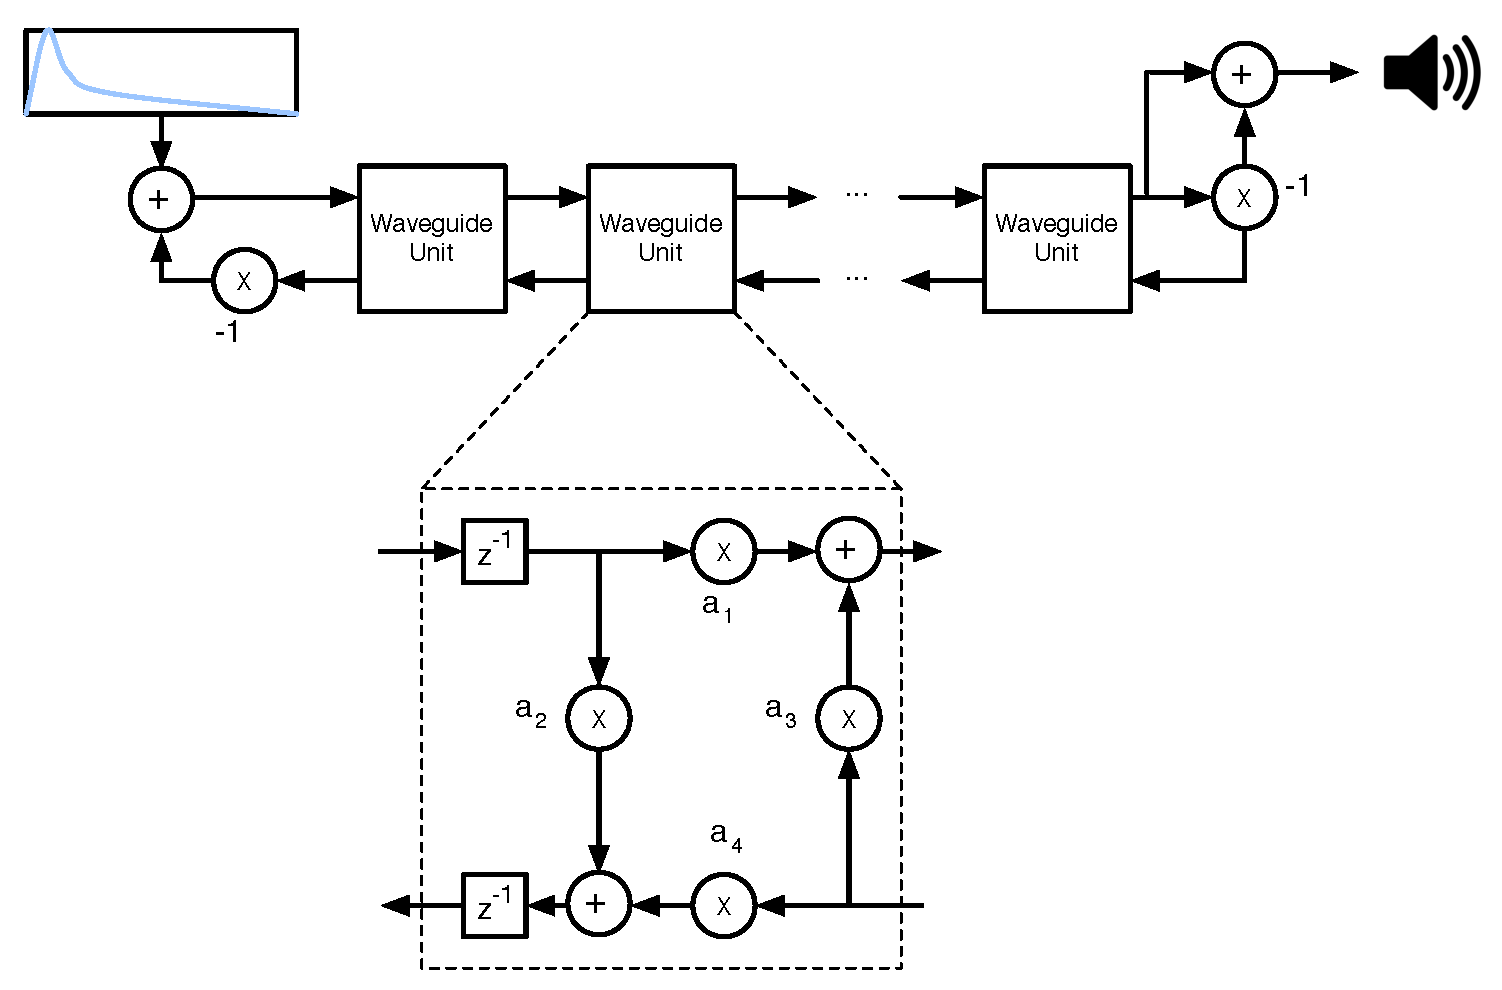
\includegraphics[scale=0.55]{DigitalWaveguideSynthesis}
\caption{Digital Waveguide Synthesis}
\end{center}
\end{figure}
The above discussion illustrates a fundamental tradeoff between versatility and control that all synthesis topologies face. The in-depth comparative study of various sound synthesis techniques, carried out by Tolonen et al., elucidates the strengths and weaknesses of each algorithm in regards to this tradeoff as well as practical issues related to implementation. However, one practical issue of utmost importance that is not covered in this study is whether each algorithm provides a mechanism by which to realize a specific target timbre. If such a mechanism does not exist, the resultant algorithm would be, at best, as useful as an instrument capable of producing any pitch and offering fine pitch control, but lacking deterministic means to produce a specific desired pitch. Chafe, in presenting a historical perspective on the many ways synthesis has influenced and benefitted composition over the last fifty years, writes that, historically, imitation has been one of the main uses of sound synthesis since its inception (1999, p. 2). Thus, the importance of being able to achieve a specific desired timbre cannot be overstated.

For sample synthesis, one only needs to record the desired sound and store it for later retrieval. However, as previously stated, as the number of desired timbres increases the storage requirements become difficult to manage and therefore more sophisticated methods are required. For the other synthesis algorithms discussed, there are unfortunately no obvious ways to extract the precise parameter set for a desired timbre. A body of research has emerged specifically to develop methods for this task. These methods are generally referred to as `parameter estimation' or `re-synthesis' techniques.

\section{Parameter Estimation}
Estimating synthesis parameters for a target timbre is a difficult problem (see Figure 2.8). Johnson and Gounaroloulos \cite{Johnson:2006pi} write that that it is not possible to find an appropriate mapping from the input parameters to a desired result unless ``[users] have a very strong understanding of the underlying mechanisms that produce the sound, or a large amount of `trial-and-error' experience with generating timbral changes within a system'' \cite[p. 1]{Johnson:2006pi}. However, even with both strong understanding of a sound synthesis algorithm's sound producing mechanisms and extensive experience using the algorithm to explore timbre, the ability to realize a particular point or region in timbre space can be time-consuming at best, and is often infeasible, as discussed in Heise et al.'s paper on parameter estimation (2009, p. 1). The requirement that a composer be versed in signal processing theory and, quite often, computer programming in order to even begin to search efficiently in timbre space is not ideal. Mitchell and Creasey (2007) note that such a requirement often leaves the composer ``more concerned with the scientific process [driving the algorithm] than artistic creativity'' (p. 1).
\\
\begin{figure}[h!]
\begin{center}
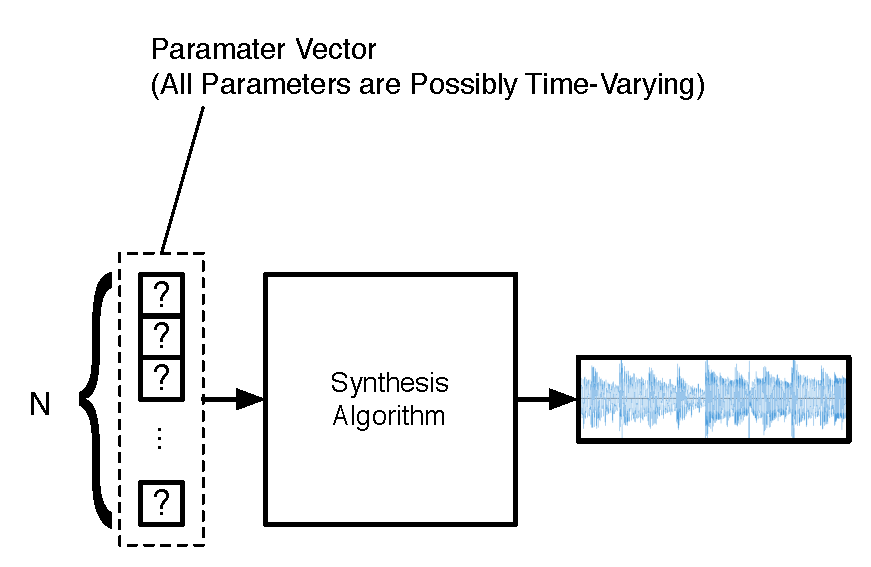
\includegraphics[scale=0.7]{ResynthesisProblem}
\caption{The Task of Producing a Target Timbre}
\end{center}
\end{figure}
As opposed to leaving the task of target timbre discovery to the composer, re-synthesis and parameter estimation techniques attempt to automatically fit the parameters of a sound synthesis algorithm to imitate a target sound (see Figure 2.9). Specifically, re-synthesis uses the results of a target signal's analysis to fit parameters to an underlying synthesis algorithm. Once a particular parameter fitting has been found, the user is left to explore the space around the target using the underlying synthesizer. This means that a re-synthesis technique paired with a specific synthesis algorithm will combine to produce a system that suffers from the same pitfalls associated with the algorithm. It is therefore useful to categorize re-synthesis techniques based on their underlying synthesis algorithms, so that one may compare these techniques within the proper context.
\\
\begin{figure}[h!]
\begin{center}
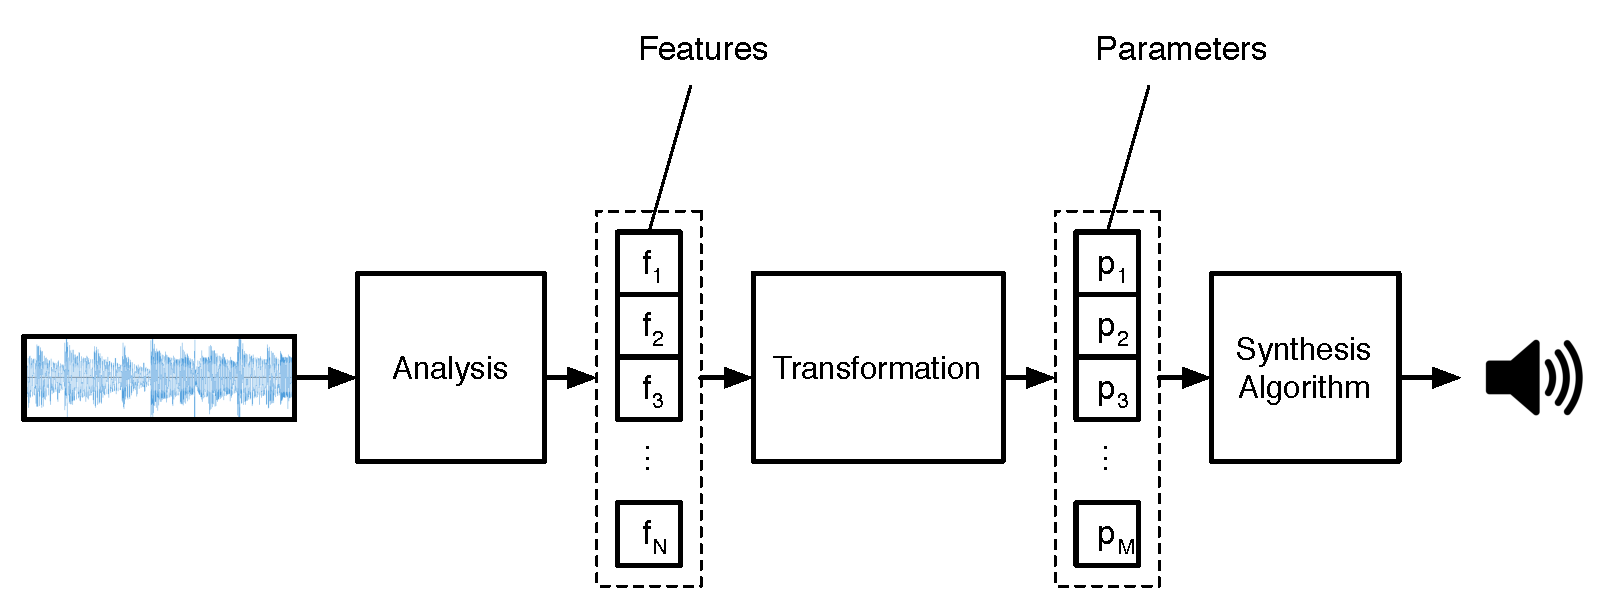
\includegraphics[scale=0.5]{ResynthesisIdea}
\caption{Re-synthesis Approach}
\end{center}
\end{figure}
An in-depth comparison of some of the most ubiquitous re-synthesis techniques can be found in Klingbeil's dissertation (2009). However, one must look beyond this source in order to evaluate promising state-of-the-art techniques from each synthesis category proposed by Smith (1991).

One of the most popular re-synthesis techniques utilizing a sampling synthesis method is concatenative synthesis (see Figure 2.10). Concatenative synthesis, as described by Diemo Schwarz, ``use[s] a large database of source sounds, segmented into units that match best the sound or musical phrase to be synthesized, called the target'' (2006, p.1). In principle, concatenative synthesis can be used to match any type of feature (e.g. pitch or loudness). To differentiate timbral matching from other objectives, the term ``musical mosaicing'' is used, a process first developed by Zils and Pachet (2001). 
\\
\begin{figure}[h!]
\begin{center}
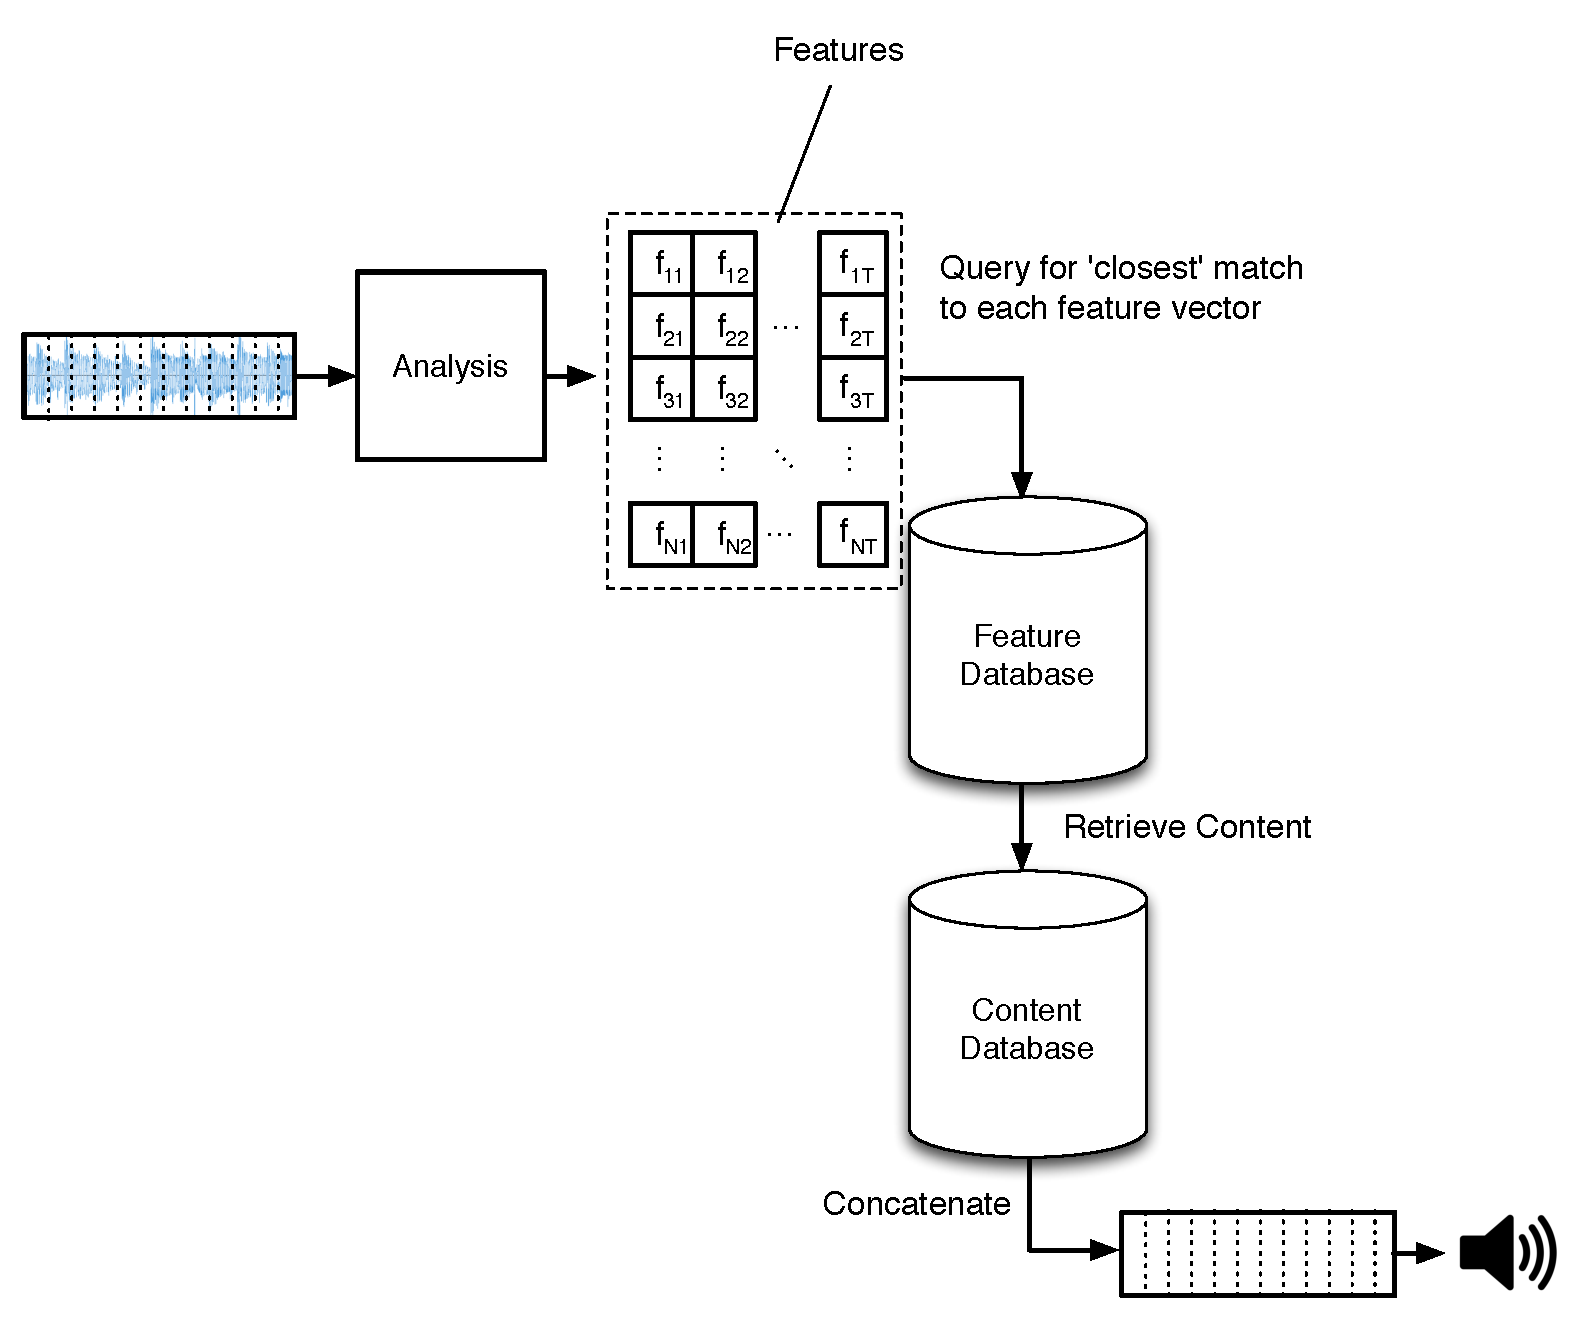
\includegraphics[scale=0.55]{ConcatSynth}
\caption{Concatenative Synthesis}
\end{center}
\end{figure}
In order to determine the best timbral match in the database to a given target one must rely on a perceptual distance measure. Deriving such a measure is complicated (as will be discussed later) (Schwarz, 2006, p. 13). In addition to searching for the best matching units, musical mosaicing also typically constrains the sequencing of these units to ensure a smooth timbral development (Zils \& Pachet, 2001, p. 1). In order to achieve accurate re-synthesis, a large database of units is required to meet both local and global constraints while providing a high-fidelity solution. As the size of this database increases an efficient search becomes difficult. The length of this search may not be problematic for a composer interested in matching one particular target, but if timbral exploration around the target is desired, the search for a new sequence for every slight timbral variation becomes a prohibitive bottleneck (Schwarz, 2006, p. 11).  If discontinuities between units and imprecise unit matching is acceptable however, such a search can usually be run in realtime.

For example, Bonada and Serra (2007) have developed a system where they pre-compute timbral features over an extremely large database of vocal sound units that sufficiently cover their vocal feature space, and allow a user to map performance trajectories to that space, retrieving the closest units to that trajectory, and concatenating them to produce an output signal. They call this `performance sampling' (p. 67).Their system is able to generate a wide variety of vocal timbral evolutions. However, as noted by the authors, the storage requirements are large in order to model only a small region of timbre space and they have yet to determine a way to limit undesirable discontinuities between `breathy to nonbreath connections' (Bonada \& Serra, 2007, p. 78).

An interesting granular synthesis re-synthesis techniques was proposed by Johnson \cite{Johnson:1998sh}. He provides a system to the user that allows them to score a number of randomly generated output sounds based on their similarity to a user-defined target. These scores are used to `push' the parameter set corresponding to each generated output towards the target sound, and the user scores the results again. This process continues until the target is reached (p. 2). The system works well as long as the user commits to the process, but because it is not completely automated, it is not an ideal solution.

There are several popular re-synthesis methods that employ spectral models, which fit the parameters of additive synthesizers. Of these, the most popular are the Phase Vocoder and Spectral Modeling Synthesis

The phase vocoder (see Figure 2.11) was developed at Bell laboratories in 1966 and first introduced to the music community as a re-synthesis tool a decade later by Moorer (1978). It makes use of the spectral representation of a target sound provided by a short-time Fourier transform (STFT). This technique uses the phase spectra returned by the STFT to provide better estimates for the frequency values associated with each bin. These values along with the magnitudes and phases corresponding to each bin can be used to set the parameters of an additive synthesizer. If the sound is harmonic or quasi-harmonic (i.e. contains little noise), then one can convincing re-synthesize the sound using a small number of peaks for a more efficient implementation. 
\\
\begin{figure}[h!]
\begin{center}
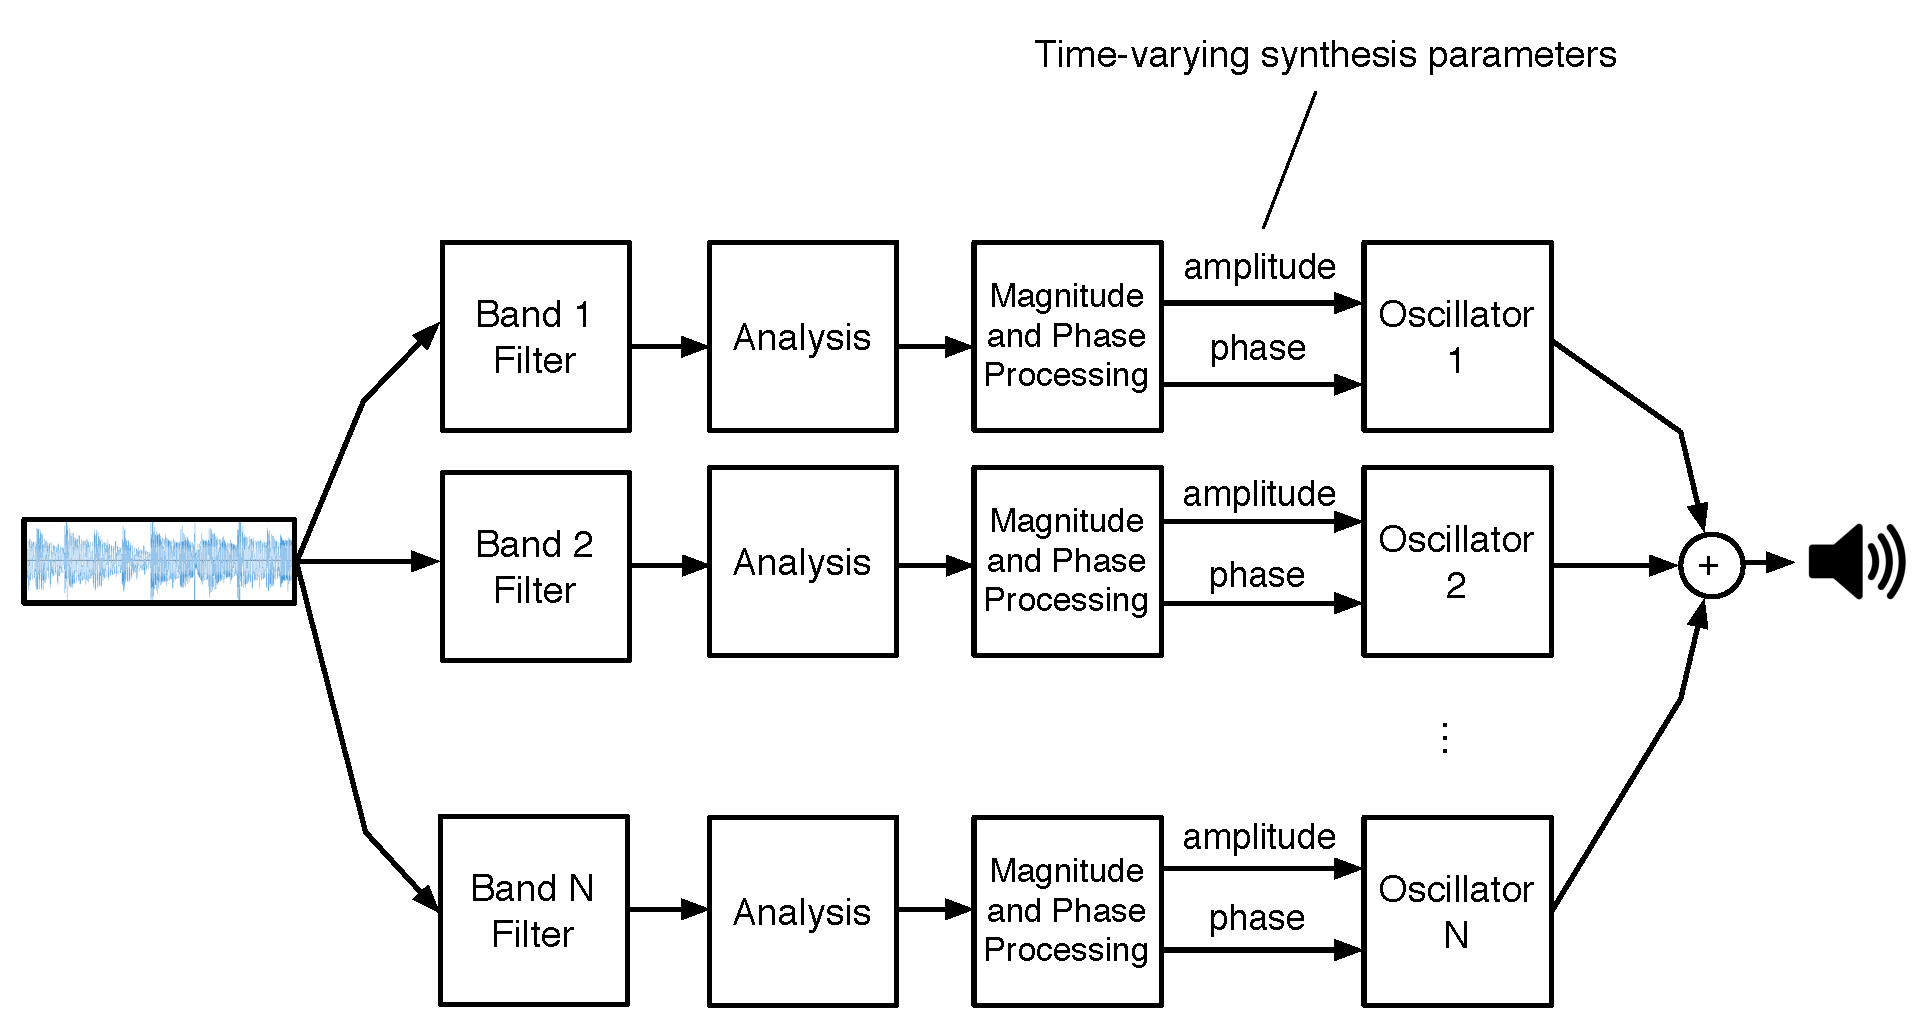
\includegraphics[scale=0.45]{PhaseVocoder}
\caption{Filter-bank Implementation of the Phase Vocoder}
\end{center}
\end{figure}
There are two main problems with the phase vocoder. First, transients are often very difficult to model accurately. Robel has been working on this problem for a number of years (2003, 2010) and made good progress, but notes that it is still an unsolved problem (2010, p. 1). Second, the phase vocoder performs poorly on ``inharmonic sounds with deep vibrato'' due to its inability to track frequency components across bins and its difficulty in efficiently modeling noise (Serra \& Smith, 1990, p. 13). This second problem was the impetus to the development of Spectral Modeling Synthesis (SMS) by Serra and Smith (1990).

Spectral Modeling Synthesis (SMS) (see Figure 2.12) ``models time-varying spectra as a collection of sinusoids controlled through time by piecewise linear amplitude and frequency envelopes [the deterministic part] and a time-varying filtered noise component [the stochastic part]'' (Serra \& Smith, III, 1990, p. 12). The deterministic portion contains sinusoids that are able to change in frequency, via partial tracking methods, but as stated, these changes are represented by piecewise linear functions, which ``affects the generality of the model'' (Tolonen et al., 1998, p. 31). Transients are also difficult to model. This has led to the development of an extended technique called Transient Modeling Synthesis (TMS), which ``provides a parametric representation of the transient components'' (Tolonen et al., 1998, 33). However, TMS requires the accurate segmentation of transients from a given signal, which is a difficult problem in its own, as discussed in \cite[p. 16]{Ciglar:2009uf}. Additionally, Serra and Smith note that:

\begin{quote}
%\linespread{1}
\selectfont
the characterization of a single sound by two different representations may cause problems. When different transformations are applied to each representation [which is common in order to transform the target sound], it is easy to create a sound in which the two components, deterministic and stochastic, do not fuse into a single entity (1990, p. 23).
\end{quote}
%\linespread{1.7}
\selectfont

Klingbeil adds that ``partial tracking becomes particularly difficult in the presence of noise, reverberation, or dense polyphony'' and also that SMS ``requires a number of input parameters [that] can have a significant effect on the quality of the analysis'' (2009, p. 42).
\\
\begin{figure}[h!]
\begin{center}
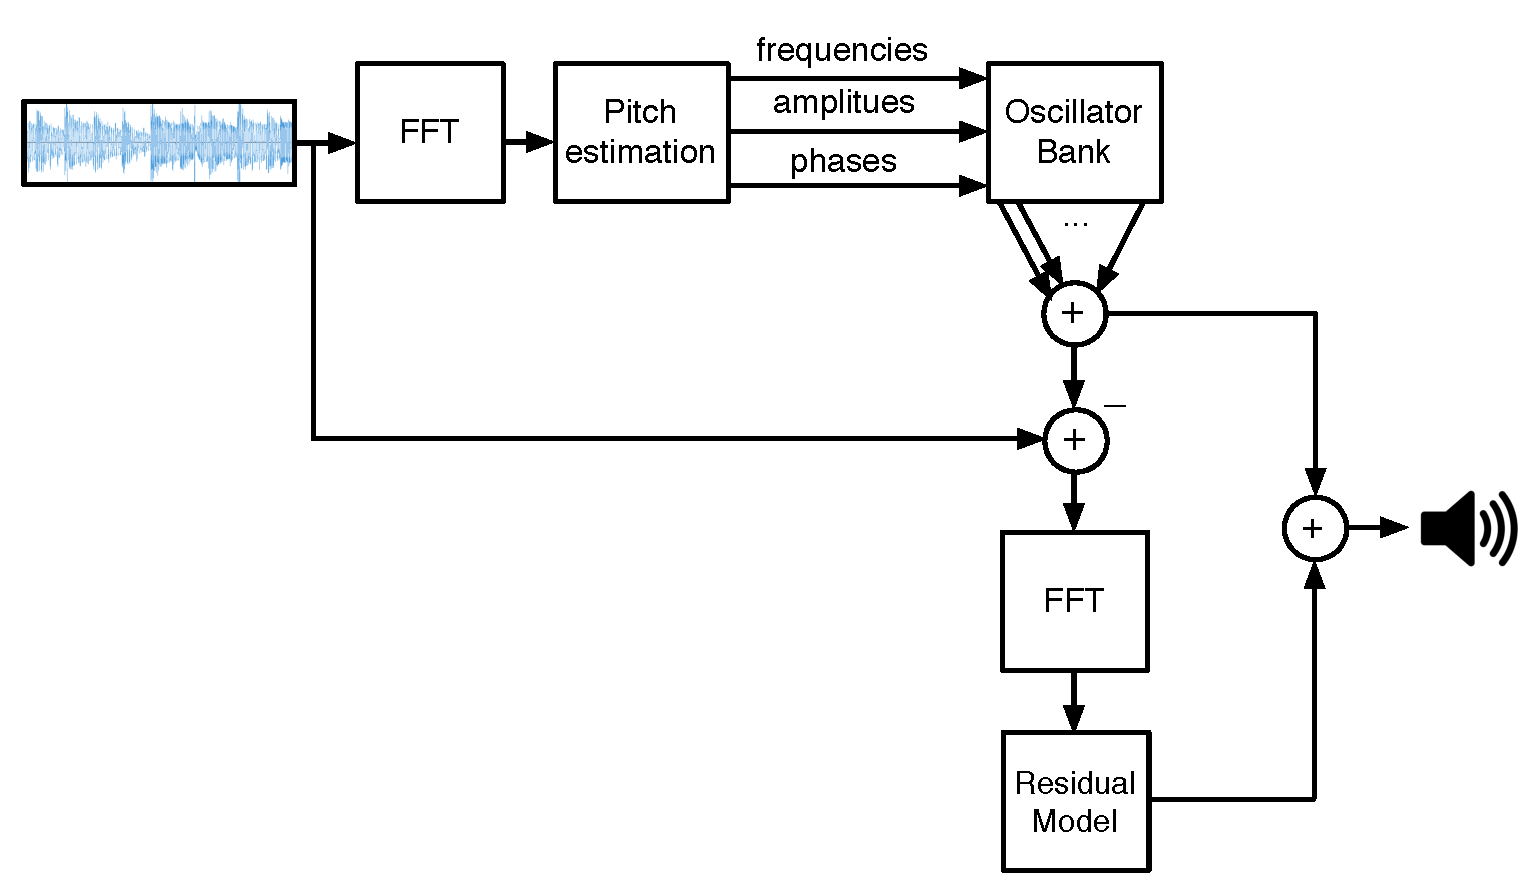
\includegraphics[scale=0.55]{SMS}
\caption{Spectral Modeling Synthesis (SMS)}
\end{center}
\end{figure}
While there has been less work produced on re-synthesis methods that overlie physical models, and abstract algorithms like FM Synthesis, some interesting research has developed in the last decade.

Vercoe, Gardner and Scheirer point out that physical modeling (e.g. digital waveguide) parameter estimation `has a particular advantage over equivalent estimation for additive, FM, or other abstract synthesis models in that the resulting parameter set has a clearly understandable interpretation, which aids in further signal manipulation' (1998, p. 11). This is due to physical modeling's low-dimensional and intuitive parameter set. Bensa, Gipouloux, and Kronland-Martinet estimate the parameters for a piano hammer-string model by analyzing a time-frequency representation of a recorded piano tone. Because the mapping of the time-frequency representation to the parameter values is complex, the authors used nonlinear optimization techniques---specifically simulated annealing, which will be discussed later---to search through the parameter space for the appropriate parameter set (2005, p. 499). A similar study was performed by Riionheimo and Vallimaki, who used nonlinear optimization techniques to estimate the parameters of a plucked string physical model (2003). Parameter estimation for physical models is a promising area of research for recreating the sounds that the models are designed for, but due to the high specificity of each model, these techniques will not be applicable outside of a small region of timbre space.

Techniques developed for re-synthesis based on frequency modulation are often referred to as ``adaptive-FM'' or ``FM-matching'' techniques (see Figure 2.13). The first researchers to successfully re-synthesize sounds using FM Synthesis were Horner, Beauchamp, and Haken (1993). Similar to physical modeling, the relationship between FM synthesis' parameter space and its output's time-frequency representation is unclear. Thus, Horner et al. also made use of a nonlinear optimization technique, a genetic algorithm (GA), to search for an optimal parameter set given a target. In these initial experiments, the parameters were not allowed to vary over time, limiting the applicability of the system (Horner et al., 1993, p. 22). This system has been extended via a number of studies outlined in Horner (2003). One of the more successful FM-matching systems, developed by Mitchell and Sullivan, matches time-varying FM synthesis parameters to various complex sounds using GAs (2005). The FM topographies used were allowed to be more complex than one with a single modulator and carrier signal (e.g. the \emph{double modulator} design uses the sum of two modulators to vary the carrier signal's frequency).
\\
\begin{figure}[h!]
\begin{center}
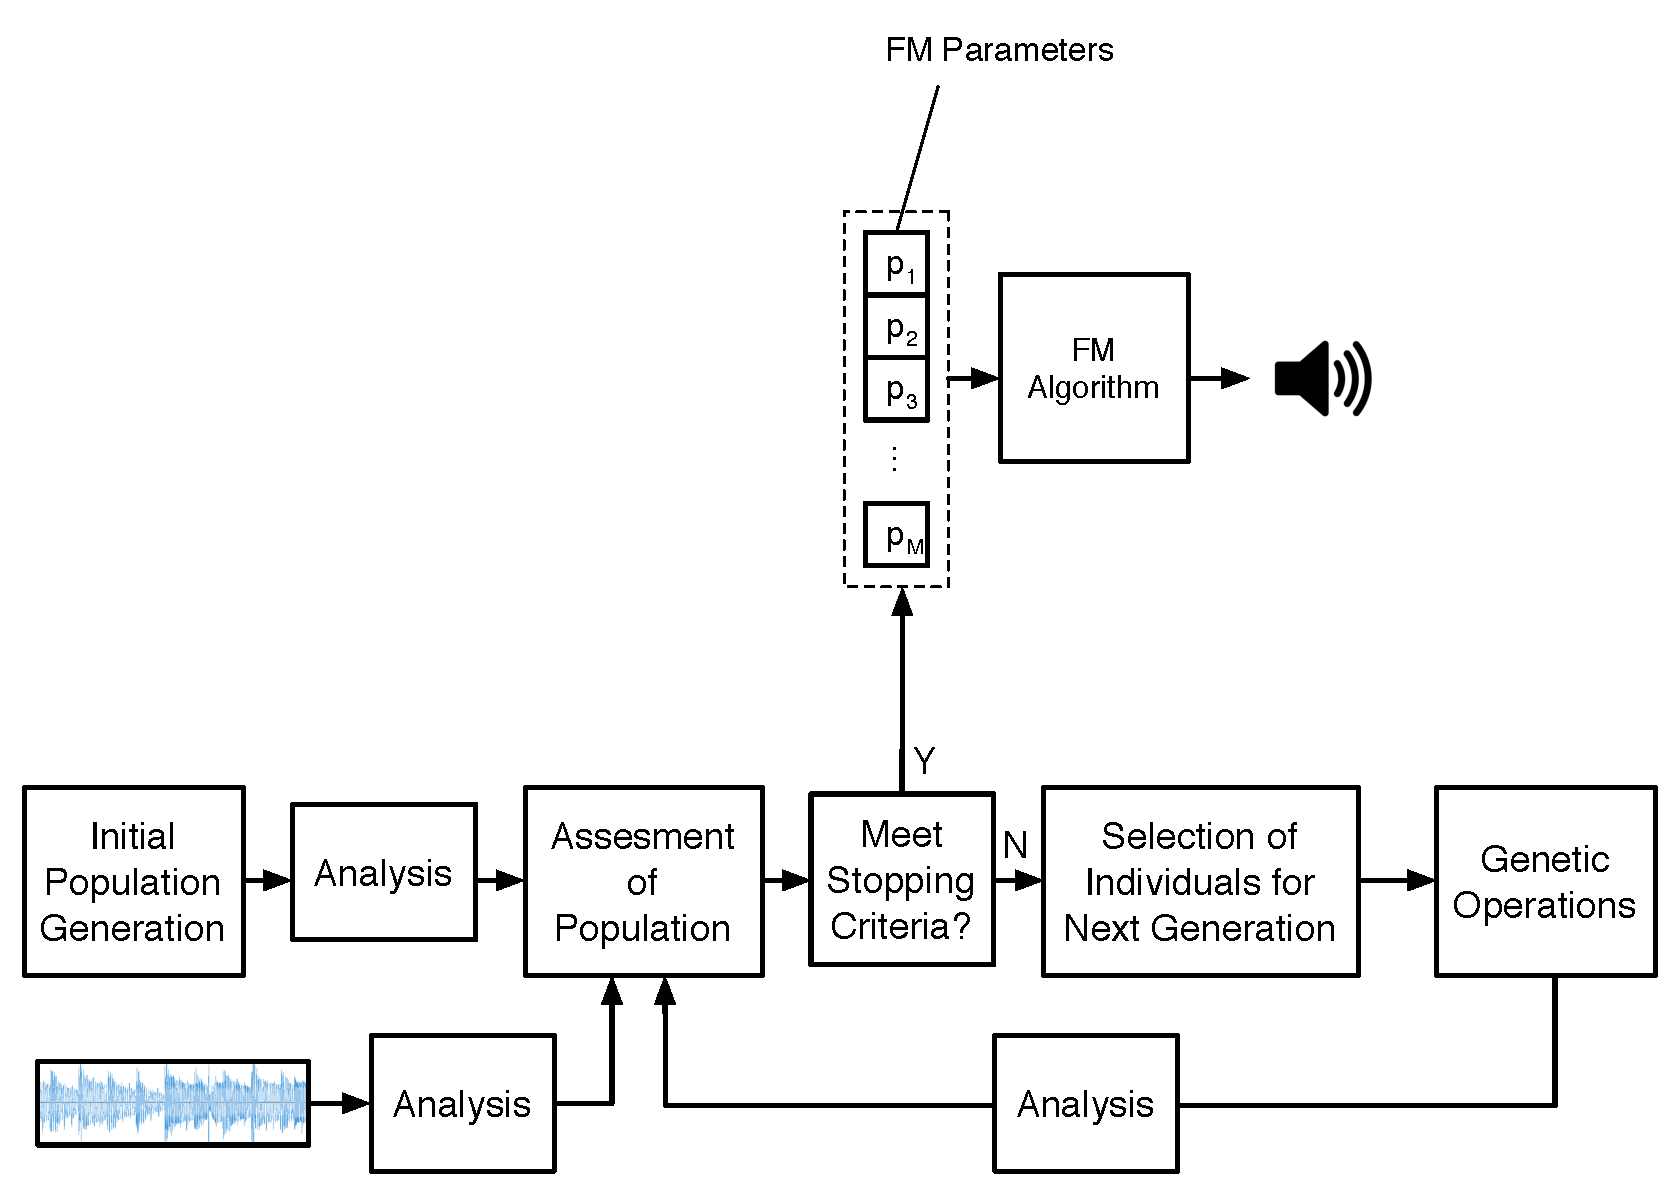
\includegraphics[scale=0.50]{AdaptiveFM}
\caption{Adaptive FM using Genetic Algorithms}
\end{center}
\end{figure}

\section{Meta-synthesis}

The previous discussion of the most popular re-synthesis methods had a common theme: each re-synthesis technique discussed is used to fit parameters to one specific synthesis algorithm. As Garcia points out (and as reiterated in (Tolonen et al., 1998, p. 103)), ``it is known that different sound synthesis techniques perform better with different types of sounds'' \cite[p. 1]{Garcia:2001jw}. Therefore, depending on the target sound, ``some parameter matching techniques can give poor results when using a fixed topology'' \cite[p. 1]{Garcia:2000th}. In other words, a re-synthesis technique that rests on top of a specific synthesis algorithm will inherit its undesirable features and therefore will be optimal for only certain types of sounds. One solution, as proposed by Misra and Cook \cite{Misra:2009km}, is to use a different synthesis algorithm (and therefore a different re-synthesis technique) for different kinds of sounds, so that each sound is generated by an algorithm that best suits it (see Figure 2.14) \cite[p. 1]{Misra:2009km}. However, knowing which algorithm to choose is often not obvious and, therefore, placing the burden of this choice on the composer is not ideal. In their concluding comments, directly related to this issue, Misra and Cook write that a way to relieve this burden would be to ``present the entire range of [synthesis] techniques to the machine and let it decide which to use on-the-fly''  \cite[p. 5]{Misra:2009km}. Such a system would require the machine to `learn' which synthesis algorithms (and corresponding re-synthesis techniques) are best suited for which kinds of sounds. However designed, the learning machine used would have to be trained on enough timbral data to sufficiently blanket timbre space. Also, one must develop a metric by which to measure how `suited' each algorithm is for each sound, so that one may be assigned the `winner.' If such a process were possible, the winners of each point in timbre space would aggregate their points into `regions' within which they lay claim as the appropriate synthesis technique to use. However, the issues of generating sufficient training data and measuring suitability of not just the synthesis algorithm, but also its paired re-synthesis technique (for a given point in timbre space) are not trivial.
\\
\begin{figure}[h!]
\begin{center}
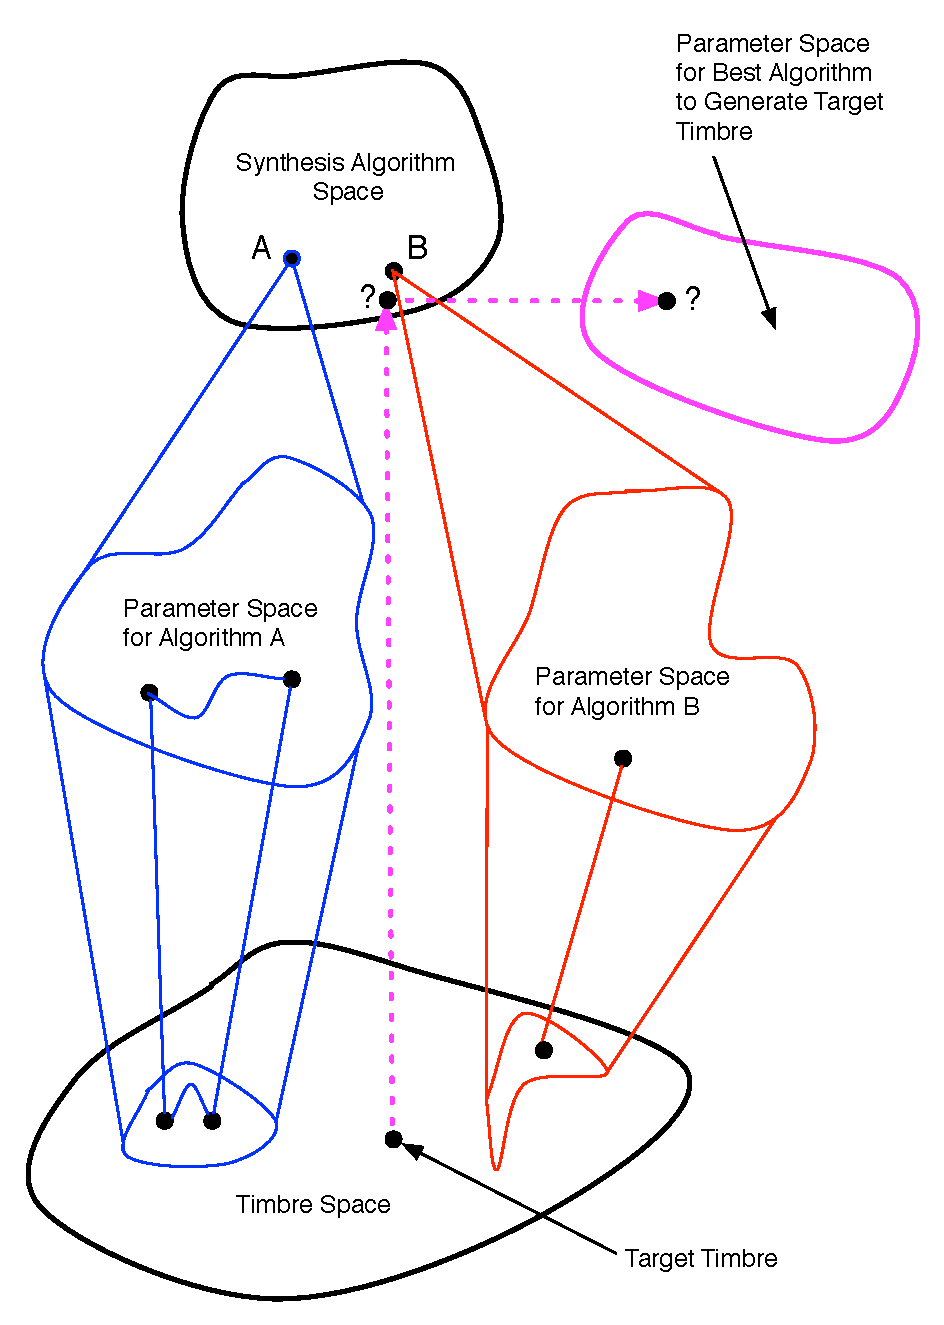
\includegraphics[scale=0.80]{MetaSynthesis1}
\caption{The Meta-Synthesis problem}
\end{center}
\end{figure}
Instead of having to generate and provide enough timbral data to blanket timbre space, Puckette (2004) proposes an alternative method for designing such a system (see Figure 2.15). First, the author defines an 11-dimensional objective timbre space by segmenting a spectrum's magnitude into 11 bands, calculating the loudness in each, and then transforming the result so that these values are decorrelated (p. 1-2). He then uses a specific synthesizer to generate points in this timbre space by sufficiently blanketing the input parameter space. When a target sound - corresponding to a path in the timbre space - is provided to his system, it re-synthesizes the sound by finding the synthesizer's nearest neighbors (using Euclidean distance) to each point in the target path, determining the `smoothest' trajectory through these nearest neighbors, and mapping this trajectory back to parameter space to determine how the synthesis algorithm can best produce the target (p. 3). Puckette notes that since his system was initially produced to force a specific synthesizer to produce the target, there may be no nearby synthesis points to the target curve (p. 3). However, one could easily extend Puckette's system by using a number of different synthesizers to produce points in timbre space and then, for a given target, constrain the match trajectory to pass only through points of one synthesizer, so that the resultant parameter set would correspond to the synthesizer which `best fits' the target. Note that this extended version of Puckette's system would also separate the suitability of the synthesis algorithm from its specific re-synthesis technique, because the re-synthesis process would be the same for all synthesis methods. Therefore, the proposed extended version of Puckette's system would solve many of the issues previously posed when developing a learning machine able to intelligently choose between synthesis algorithms. However, it is not without its own set of problems. First, it is not clear that euclidean distances in Puckette's objective timbre space are semantically meaningful. Second, there is no indication for when one has sufficiently blanketed the input parameter space of a given synthesizer. Third, a smooth trajectory of points in timbre space does not necessarily lead to a smooth trajectory to points in the parameter space. Since trajectories are drawn through a finite set of points in the timbre space, one must determine how best to interpolate between parameter sets in the input space, which, depending on the mapping, could produce wild fluctuations between points back in timbre space. Fourth, no matter how many synthesizers are provided to the system, it is not guaranteed that all points that are mapped from the various parameter spaces to this timbre space will have close neighbors. Lastly, it is not necessarily the case that the match trajectory will correspond to the `best suited' synthesis algorithm, because many algorithms have high-dimensional and non-intuitive parameter spaces, and therefore, while they may provide a best fit to the target trajectory, they may provide more a complicated exploration than another algorithm with the next best fit.
\\
\begin{figure}[h!]
\begin{center}
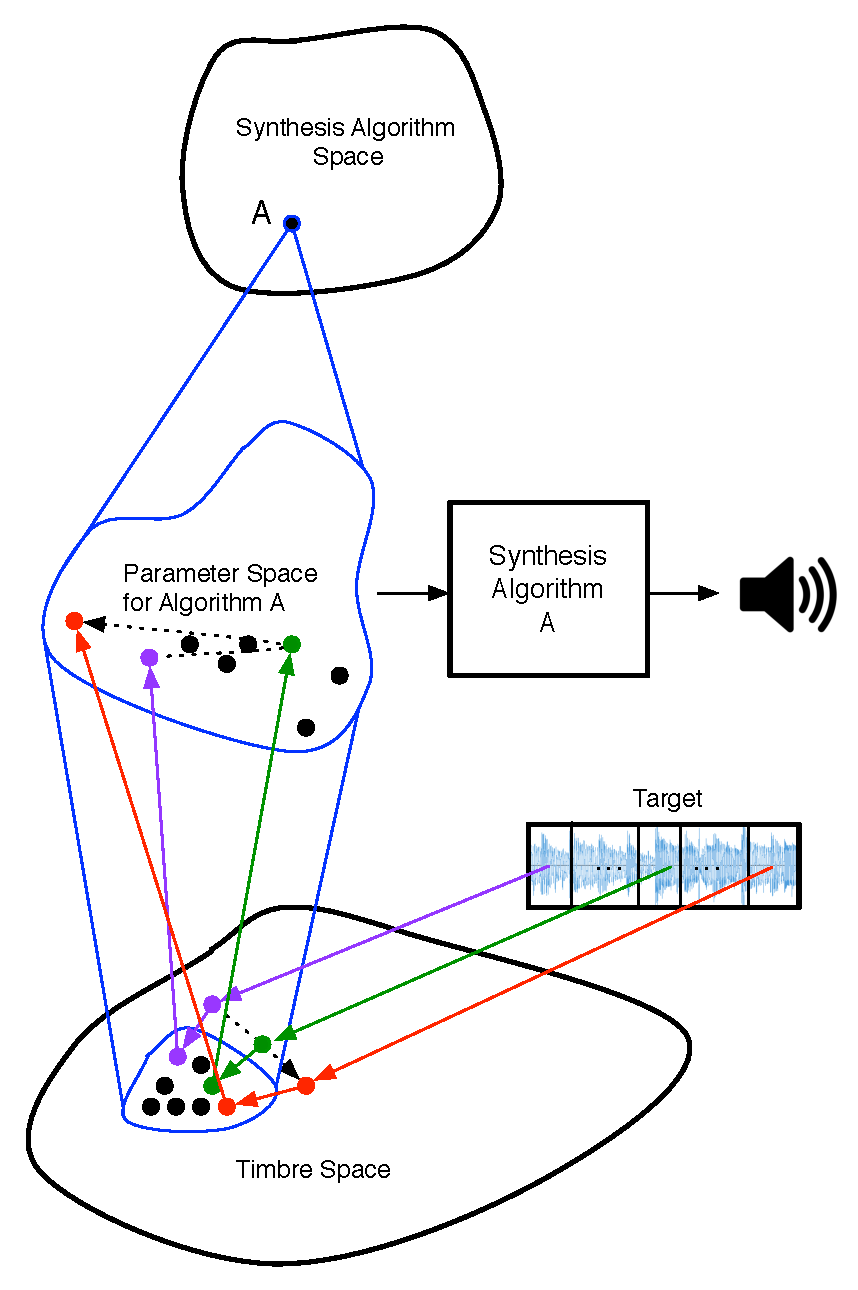
\includegraphics[scale=0.75]{PucketteMetaSynthesis}
\caption{Finding the closest parameter mappings in a partially canvassed objective timbre space.}
\end{center}
\end{figure}
Loviscach's work (2009) on making synthesizer control feel more natural for synthesizers with large parameter spaces provides a solution to this last problem. In his work, Loviscach studies correlations between parameter sets for a given synthesizer based on a database of preset data. If two different parameters are highly correlated over a broad range of parameter presets, then adjusting one will adjust the other (p. 1). Correlations are found between all pairs of parameters and placed in a two-dimensional field such that highly correlated parameters are placed next to each other. The manipulation of any one parameter will affect all others according to their distance and joint statistics (p. 1). Therefore, assuming that the provided presets for a given synthesizer correspond to a synthesizers natural usage, this system is able to replace a synthesizer's high-dimensional non-intuitive parameter space with a more natural low-dimensional one. Of course, this requires that enough presets exist for each synthesizer so that their parameter correlations can be considered statistically significant. In this case, however, a hybrid system employing techniques from both Puckette's and Loviscach's research could be quite interesting. The major hurdle would be having the enormous amount of training data necessary for both techniques to work well in harmony, making such a system impracticle. In theory, however, this hybrid system would allow a composer to provide a target timbre and, in return, would be given a specific algorithm and parameter set that they could then use to explore the surrounding space in a natural way. If further constraints are placed on storage and efficiency, this system would meet the basic requirements of an ideal synthesis tool. However, other authors have suggested that one could do even better than this.

A limitation of the synthesis learning machine proposed by Misra and Cook  \cite[p. 1]{Misra:2009km} and carried over into the previous discussion of extending Puckette's and Loviscach's systems is that the machine is only able to choose from a finite set of synthesis topologies when selecting a best-fit topology and corresponding parameter set. Suggested as early as 1998 by Vercoe, Gardner and Scheirer and supported by Garcia \cite[p. 2]{Garcia:2000th} and Moreno (2005, p. 1), hybrid synthesis methods - those allowing any combination of the `classical methods' - can provide better solutions to imitative sound synthesis both perceptually and in matters involving controllability (p. 9).

The research of Carpentier, Tardieu, Harvey, Assayag, and Saint-James (2010) exploits this same well-known fact in the domain of acoustic orchestration. They use acoustic instruments as their ``synthesis methods'' and allow any realistic linear combination of these instruments to generate a given target (see Figure 2.16). The re-synthesis problem becomes more difficult than simple parameter fitting for fixed topologies, because there is a combinatorial explosion in the number of topologies available. In order to determine an appropriate combination of instruments and associated playing techniques, they map individual instrument features (obtained from steady-state time-frequency representations) to an objective timbre space, make assumptions about how these features interact in the presence of polyphony, and perform a search over all possible combinations for that which best achieves the target (p. 2). The authors limit their system to steady-state sounds and suggest that a way to transition between timbres is to do so incrementally, with one instrument dropping out or modifying its state at a time. Such transitions would be limited in how ``smooth'' one perceives them to be as well as how quickly they may occur. However, a system utilizing this idea and based on linear combinations of synthesis algorithm's may be able to avoid this problem.
\\
\begin{figure}[h!]
\begin{center}
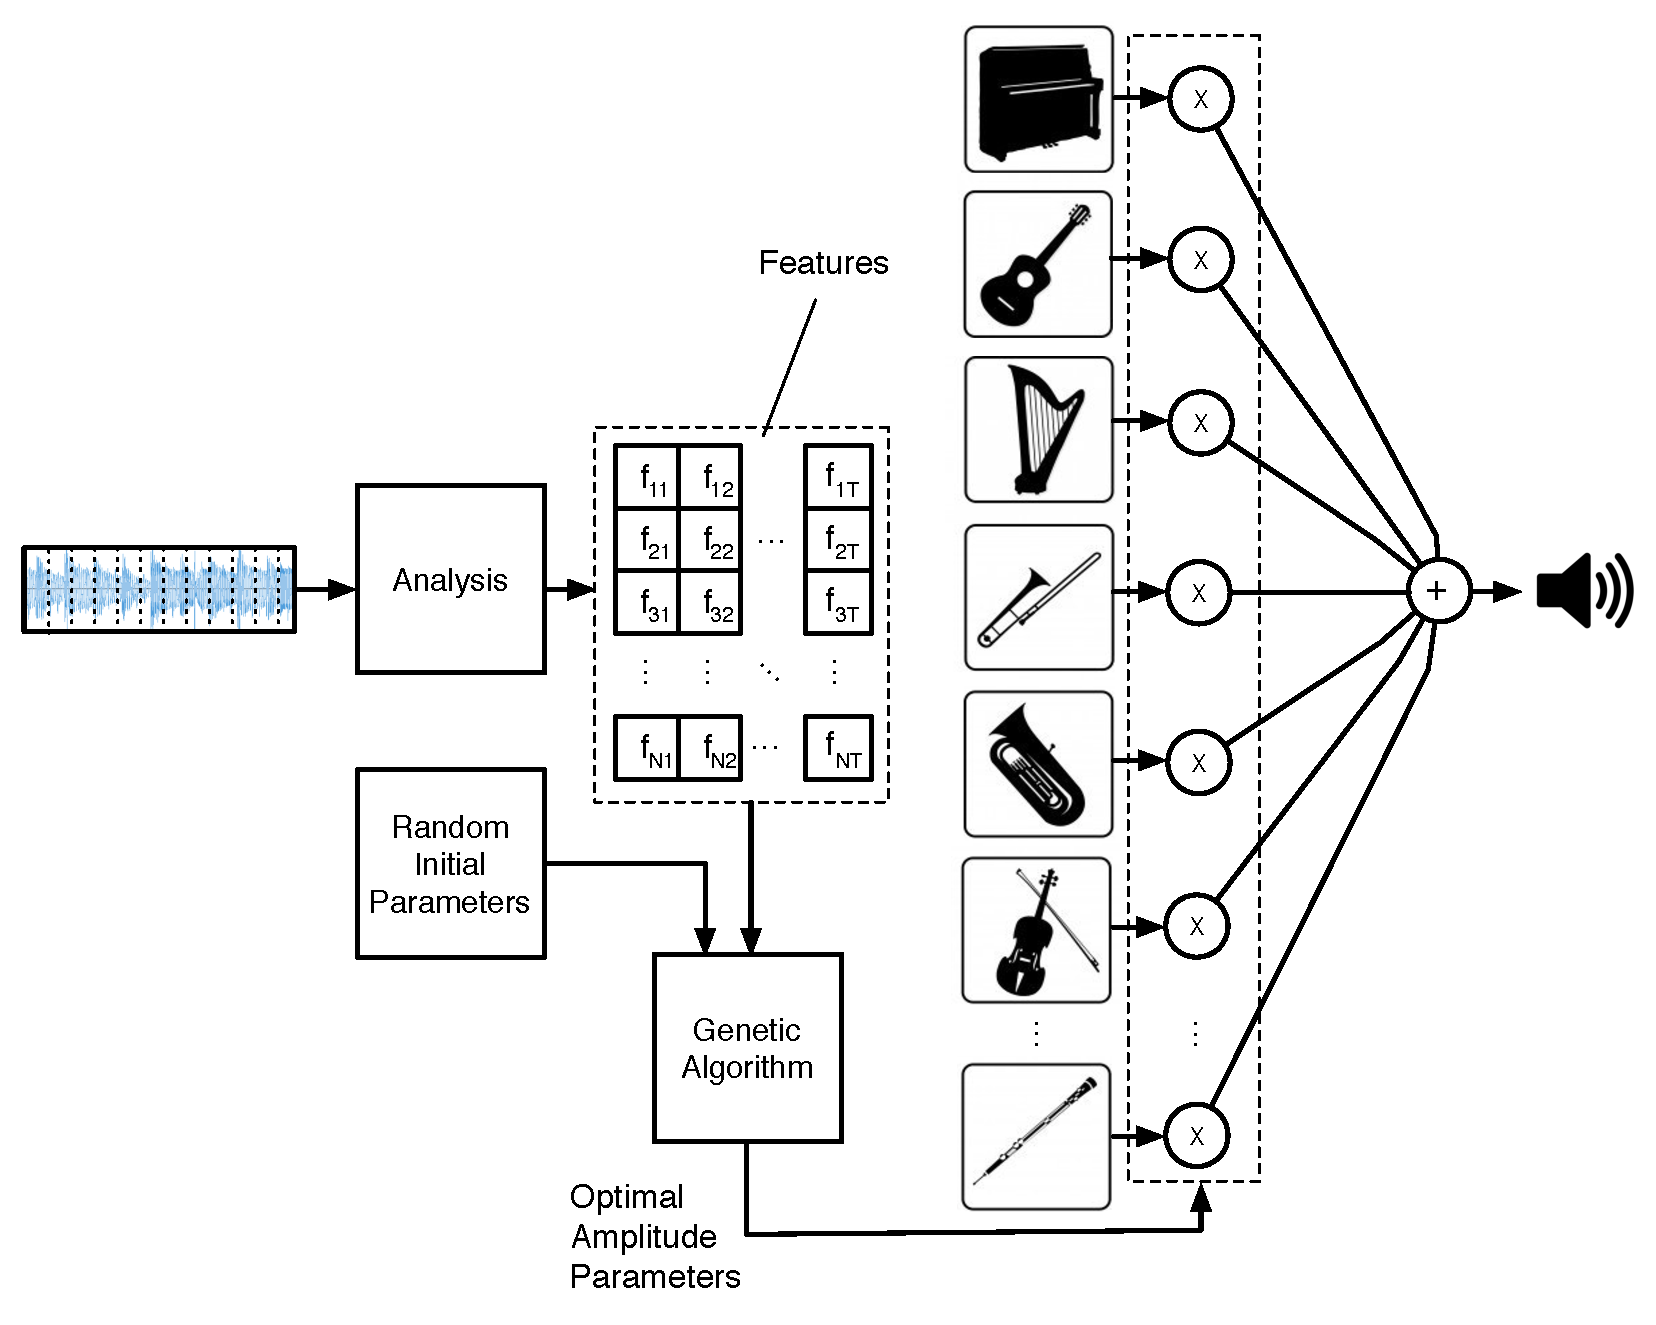
\includegraphics[scale=0.55]{OrchestralMetaSynthesis}
\caption{Approximating a complex timbre using a linear combination of orchestral instrumentation.}
\end{center}
\end{figure}
Carpentier et al. (2010) designed their system specifically as an auto-orchestration mechanism for given target sounds, constraining their search to a realizable orchestral combination. This constraint need not be applied when combining sound synthesis algorithms. It is also not necessary to consider typical sound synthesis algorithms as ``atomic'' units, as it is in the acoustic instrument case. By removing this limitation, one may be able to generate better-suited synthesis algorithms for a given target using building blocks at a different level of abstraction. Replacing high-level blocks with the lower-level components that make them up, one would be able to generate solutions at least as fit as any of those generated using the higher-level set, and possibly better \cite[p. 2]{Garcia:2000th}. However, the search space becomes larger as the atoms become lower-level and, therefore, the search itself becomes more difficult. Thus, one must balance the theoretical ability of the system to produce possibly better solutions with the practicality of being able to find one of these solutions. A few studies have attempted to build a system capable of constructing synthesis algorithms, well-suited to a given target, via an intelligent, directed search through synthesis algorithm space \cite{Wehn:1998bh, Garcia:2000th, Garcia:2002cq}. Before being able to discuss this research, one must understand the search strategy used in both studies: genetic programming (GP).

\section{Artificially Intelligent Music Systems}

An exhaustive search over synthesis space is not possible, no matter how large the atomic topology unit. Even when this search is restricted over one single topology, the parameter space will often be enormous. Therefore, it is necessary to investigate intelligent ways of searching such a high-dimensional and complex space. In order to develop a directed search technique, one must consider a way to measure how well each point in the input space performs at the given task. The resultant measure is typically represented by an ``objective function'' that, given a point in the input space, produces a value (often between 0.0 and 1.0) that represents how well the point meets the target objective. The optimal solution to the problem will exist as a global maximum along the objective function's surface (see Figure 2.17). The closed-form representation of this function is often unknown, making search difficult. However, in some cases, one can make reasonable claims about the shape of the objective surface.
\\
\begin{figure}[h!]
\begin{center}
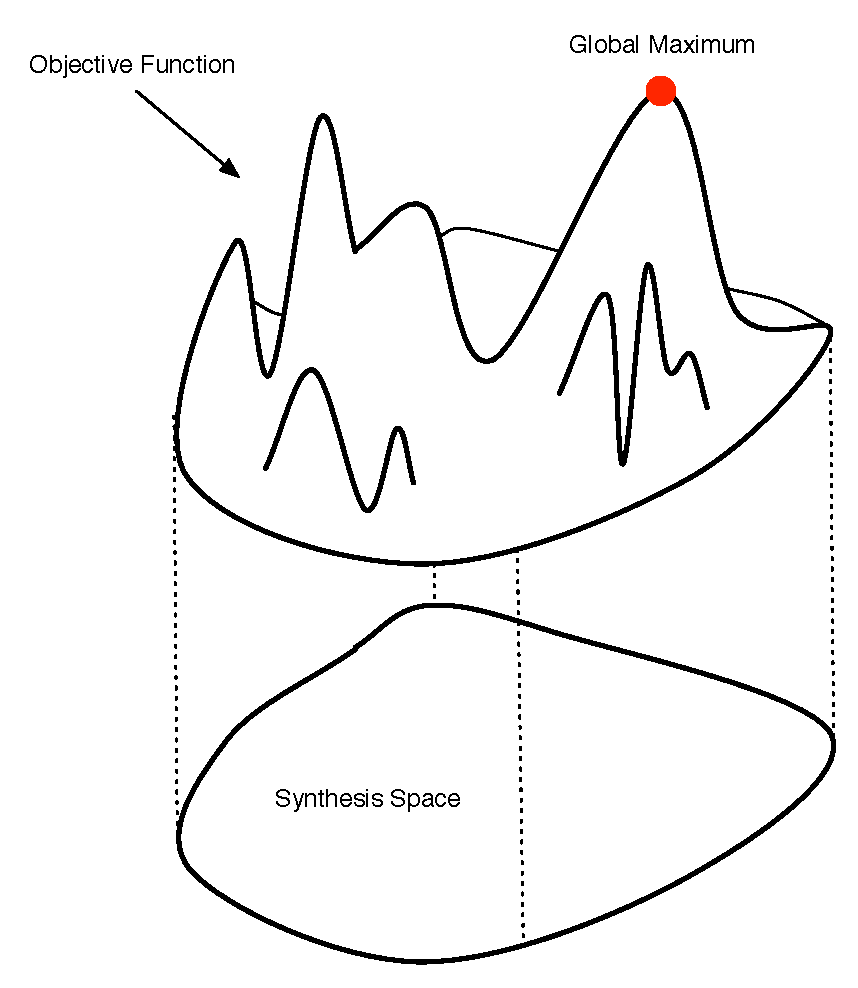
\includegraphics[scale=0.7]{FitnessFunction}
\caption{An objective function/surface sitting above synthesis space with its global maximum shown.}
\end{center}
\end{figure}
The artificial intelligence community has developed various intelligent search algorithms to address such problems, which direct the search based on hypotheses about the objective surface's shape (see Figure 2.18), and/or restrict the region of search based on known characteristics of the desired solution (Russell \& Norvig, 2009, p. 64-108).
\\
\begin{figure}[h!]
\begin{center}
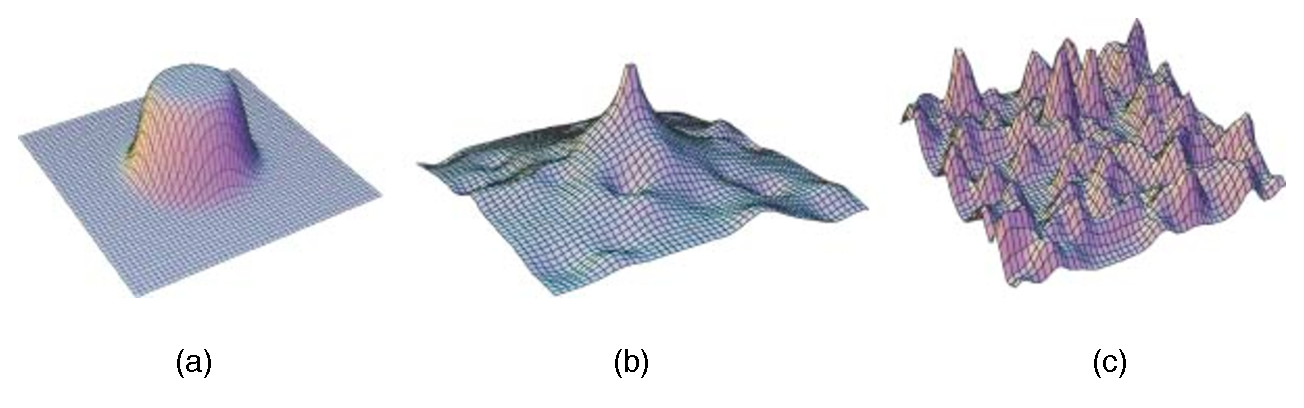
\includegraphics[scale=0.6]{DifferentTopologies}
\caption{Three different fitness surfaces: (a) unimodal and smooth, (b) multimodal, but relatively smooth and with a clear global maximum, and (c) multimodal and rough with no clear global maximum.}
\end{center}
\end{figure}
If one can assume that the objective surface is unimodal and smooth, then the most efficient search algorithm is called hill-climbing, which simply looks at all neighbors of the current position in the search and moves in the direction of greatest increase in the objective function. However, if the surface is not unimodal, then this algorithm has a chance of converging to a local maximum, which is undesirable. Teller writes that hill-climbing is a fully-exploitative search algorithm, meaning it ``focuses the search in the areas of the search space that have the highest known [objective] values'' (1998, p. 23). He explains that ``in search there is sometimes a trade-off between exploration and exploitation'' whereas opposed to exploitation, ``exploration means trying out options that are believed to be locally sub-optimal (in hopes that globally these options will lead to an improved solution)'' (1998, p. 23). If no assumptions about the shape of the objective surface can be made, then one must find a good balance between the exploitation and exploration in search so that premature convergence is unlikely to occur. Search strategies with this balance are often employed---and are known to be most productive---in cases where the problem domain is not well understood, and one does not know a priori about the structure of the solution, as is the case with the synthesis problem that we are facing (Vanneschi, 2004, p. 42). Thus, it is not a coincidence that variants of genetic algorithms (GA)---a strategy that provides mechanisms to directly control the amounts of exploitation and exploration---have been successfully utilized in many of the paremeter estimation studies listed above (Horner et al., 1993); \cite{Johnson:1998sh}; (Riionheimo \& Valimaki, 2003); (Mitchell \& Sullivan, 2005). The degree to which GAs have helped solve the FM matching problem has led Horner, one of the initial pioneers of FM matching, to proclaim that it has helped push FM matching ``into something of a renaissance period'' (2003, p. 28).

As described in his dissertation on making variants of GAs more efficient, Vanneschi writes that GAs ``can be imagined as operating via a population of explorers initially scattered at random across the landscape. Those explorers that have found relatively high fitness points are rewarded with a high probability of surviving and reproducing'' (2004, p. 70). (Note that when discussing GAs, the objective surface is often referred to as the ``fitness'' surface and the process of search is called ``evolution''.) The ``pull'' strength of explorers from regions with low fitness values to regions with high fitness values is determined by the GA's parameters, allowing one to specify in what ways the algorithm exploits and explores. The ability to search many different regions of the input space in parallel increases the probability of finding many local optima on a complex multi-modal fitness surface and then selecting the best option between all of them \cite[p. 37]{Garcia:2001jw}. For an visual example of how a GA might obtain a near-optimal parameter set, see Figure 2.19.
\\
\begin{figure}[h!]
\begin{center}
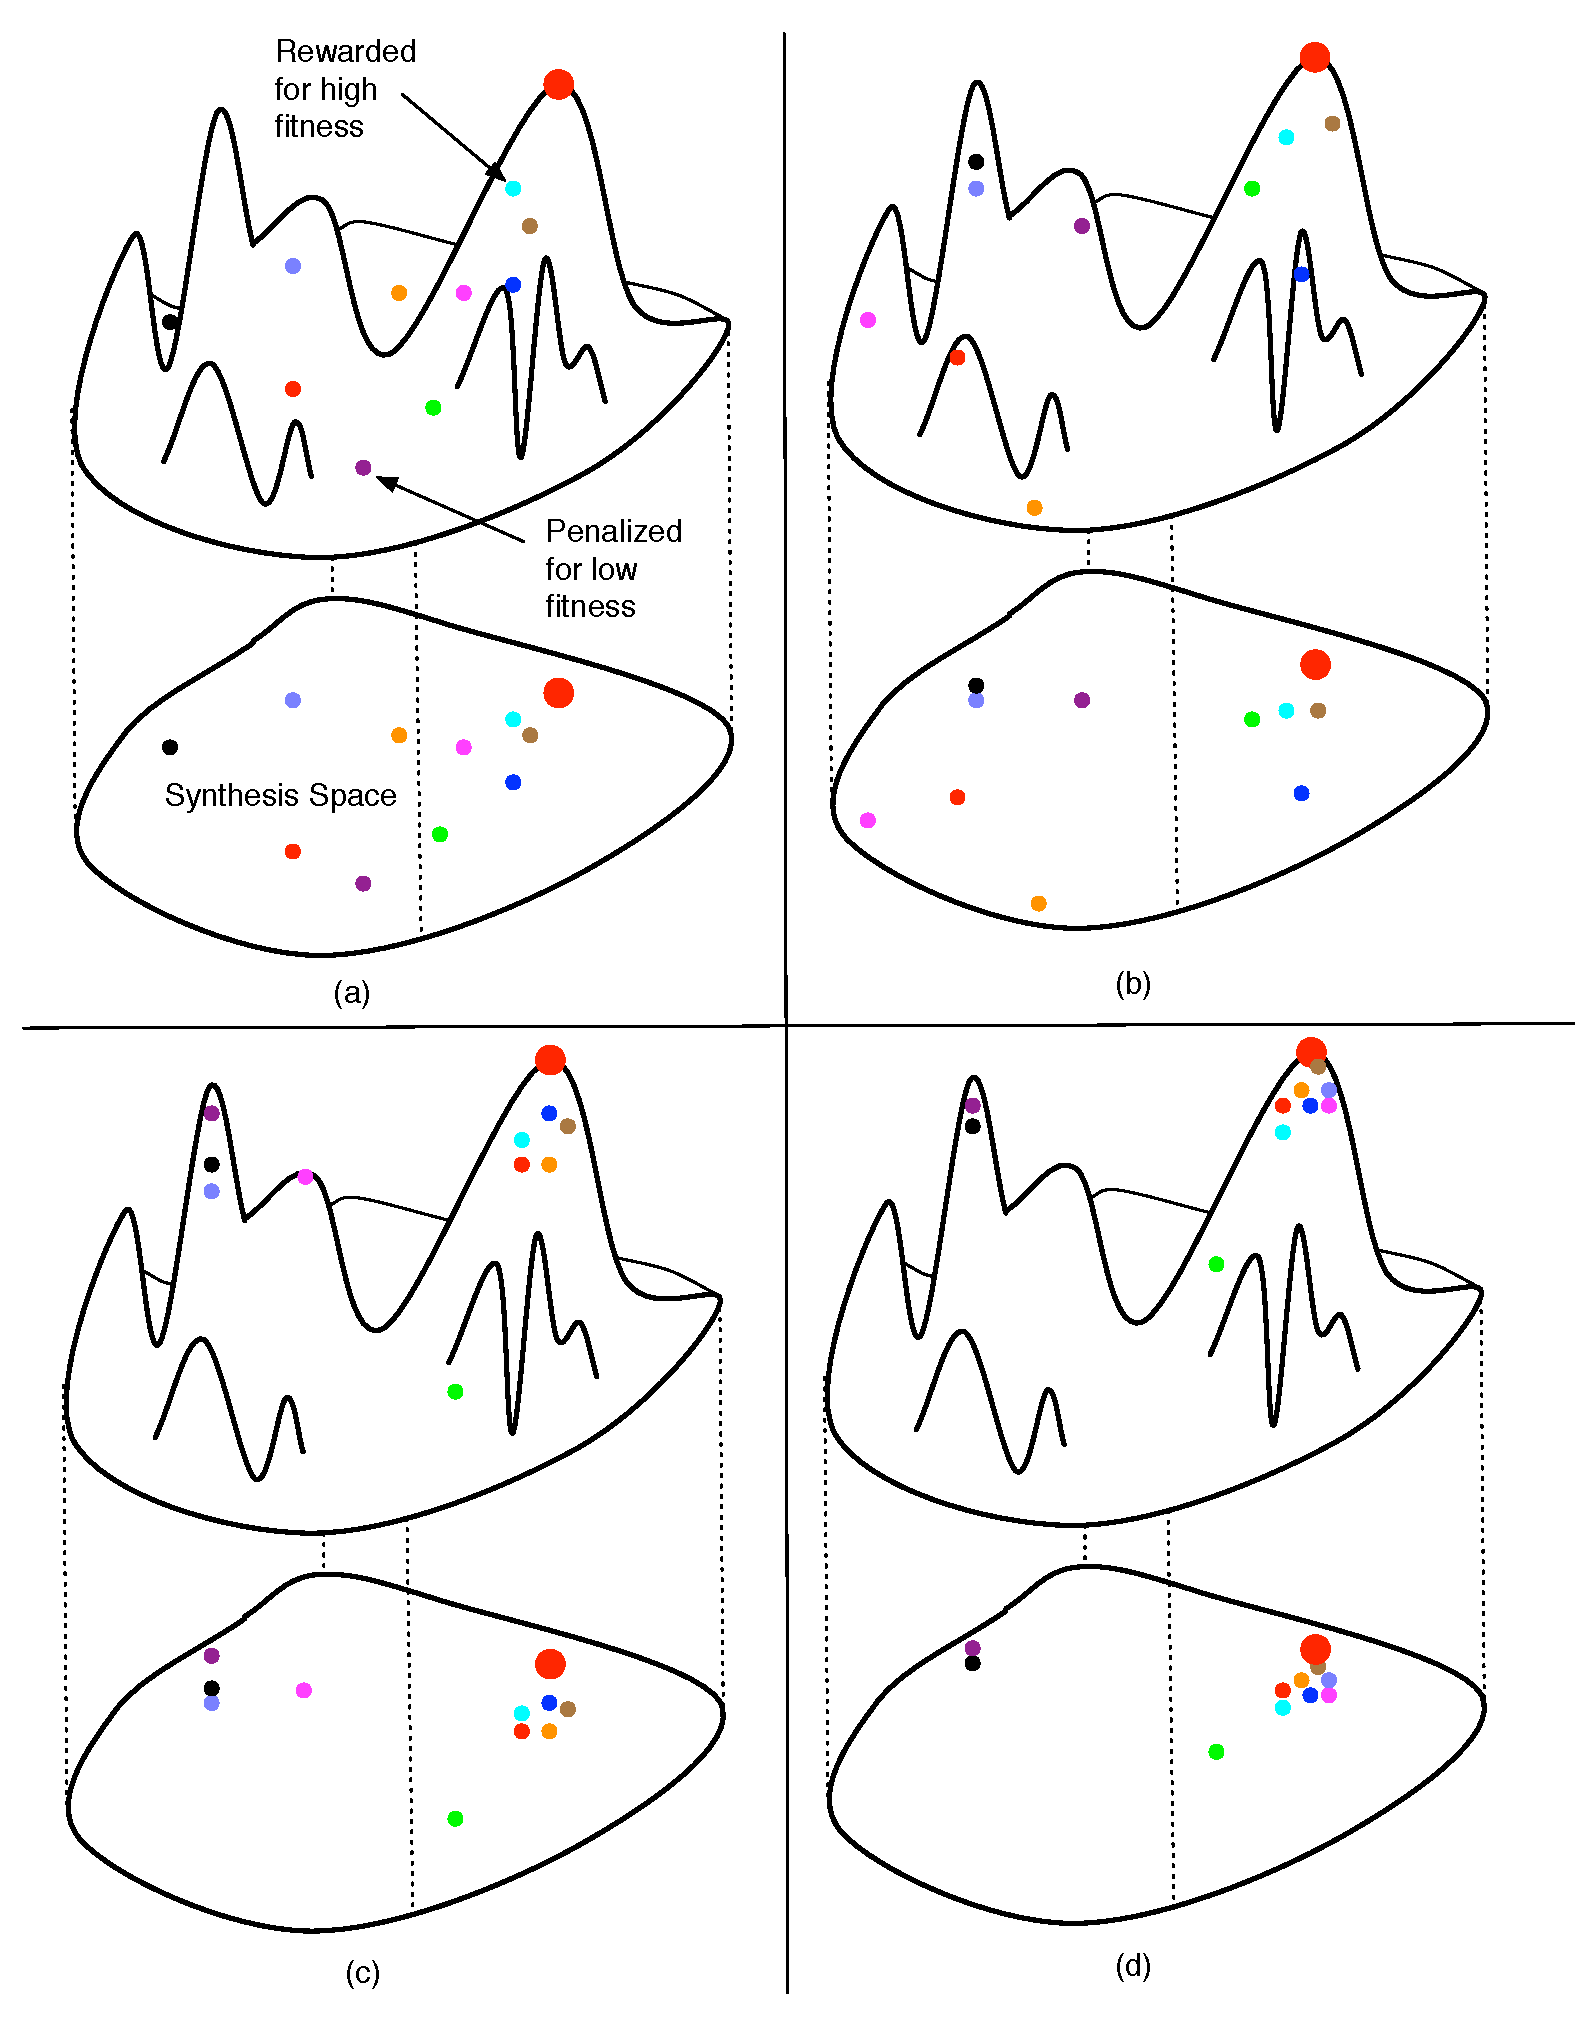
\includegraphics[scale=0.50]{GASearch}
\caption{A GA population after: (a) 1, (b) 10 (c) 100, and (d) 1000 iterations (and optimal solution notated by large red dot).}
\end{center}
\end{figure}
Since it is known that for at least several fixed topology parameter estimation techniques (e.g. FM matching, physical model parameter estimation, granular re-synthesis), the objective surfaces are best searched via genetic algorithms, it is very likely that the objective surface for the more complex problem of simultaneous topology and parameter estimation will also be best searched using genetic algorithms. However, classical genetic algorithms can only be applied when the size and shape of the solution is known beforehand (Vanneschi, 2004, p. 42). In the search for an appropriate synthesis algorithm topology, the size and shape of the ultimate solution is a large part of the problem. Research into more sophisticated search methods, which are better able to search over algorithm space is the subject matter of Automatic Programming.

``Automatic Programming is one of the central goals of computer science...[the goal being to make] computers perform required tasks without being told explicitly how to accomplish these tasks'' (Koza, Bennet III, Andre, Keane, \& Dunlap, 1997, p.3). Ideally, in an Automatic Programming system, requirements provided by the user only specify what the intended behavior of the program is and not how it should produce that behavior. In a paper overviewing the many different approaches to Automatic Programming, Rich and Waters \cite{Rich:1992sp} state that Automatic Programming has three goals: to make a system end-user oriented, general purpose, and fully automated \cite[p. 4]{Rich:1992sp}. All approaches in existence at that time focused on two of these goals at the expense of the third. Rich and Waters split these approaches into three categories: bottom-up, narrow-domain, and assistant \cite[p. 3]{Rich:1992sp}. Bottom-up approaches sacrifice the user-oriented goal and result in high-level programming languages that are general purpose and fully automated (i.e. they automatically generate machine code), with a goal of becoming ``very high level in the future'' \cite[p. 3]{Rich:1992sp}. Narrow-domain approaches focuses on a narrow domain, but is end-user oriented and fully automated, with the goal of becoming wider-domain in the future \cite[p. 4]{Rich:1992sp}. The assistant approaches lead to systems that are user-oriented and general purpose, but not fully automated (e.g. integrated development environments (IDEs)) \cite[p. 4]{Rich:1992sp}. 

The meta-synth problem suggests the need for a narrow-domain system (only designed for generating synthesis algorithms) that is end-user oriented (where the end user only needs to specify a target output) and fully automated (the synthesis topology and optimal parameter set are found and returned). These approaches typically frame the Automatic Programming problem as one of intelligently searching through algorithm space in order to find an algorithm able to produce the desired output, which falls in line with how this paper interprets the problem. The most common intelligent search strategy though algorithm space is, unsurprisingly, based on genetic algorithms and is called genetic programming (GP) (Koza, 1992). In fact, genetic programming is so ubiquitous in Automatic Programming research that da Silva---in his dissertation on GP---mistakenly defines GP \emph{as} 'the automated learning of computer programs' even though it is actually a subset of Automatic Programming \cite[p. ix]{Silva:2008le}.

GP can be thought of as ``variable length, tree-based genetic algorithms'' (Teller, 1998, p. 29). The search mechanics of GP are analogous to those of GAs, meaning GP also performs a parallel search through the input space for points (re: algorithms and paired parameter values) that meet the specified fitness (re: algorithm output), balancing exploration and exploitation in a similar manner. The individual points in algorithm space are typically represented by tree data structures whose terminal nodes (or leaves) represent input parameters to the other functional node elements (see Figure 2.20). This representation was first proposed by Koza as a natural way to structure Lisp programs (1992). It has been successfully applied to a number of different programming languages since. However, there are a number of different ways to translate code to this representation as well as a number of operator variants  used to perform the search, and as pointed out by Vanneschi, ``the art of choosing an appropriate representation and an appropriate set of operators is often a matter of experience and intuition'' (2004, p. 6). Beyond choosing the representation and operators, there are also a number of GP parameters that must be set, and ``much of what GP researchers know about these parameters is [also] empirical and based on experience'' (p. 32). Progress on systematic ways of selecting specific orientations of these variables has been made recently and will be discussed below.
\\
\begin{figure}[h!]
\begin{center}
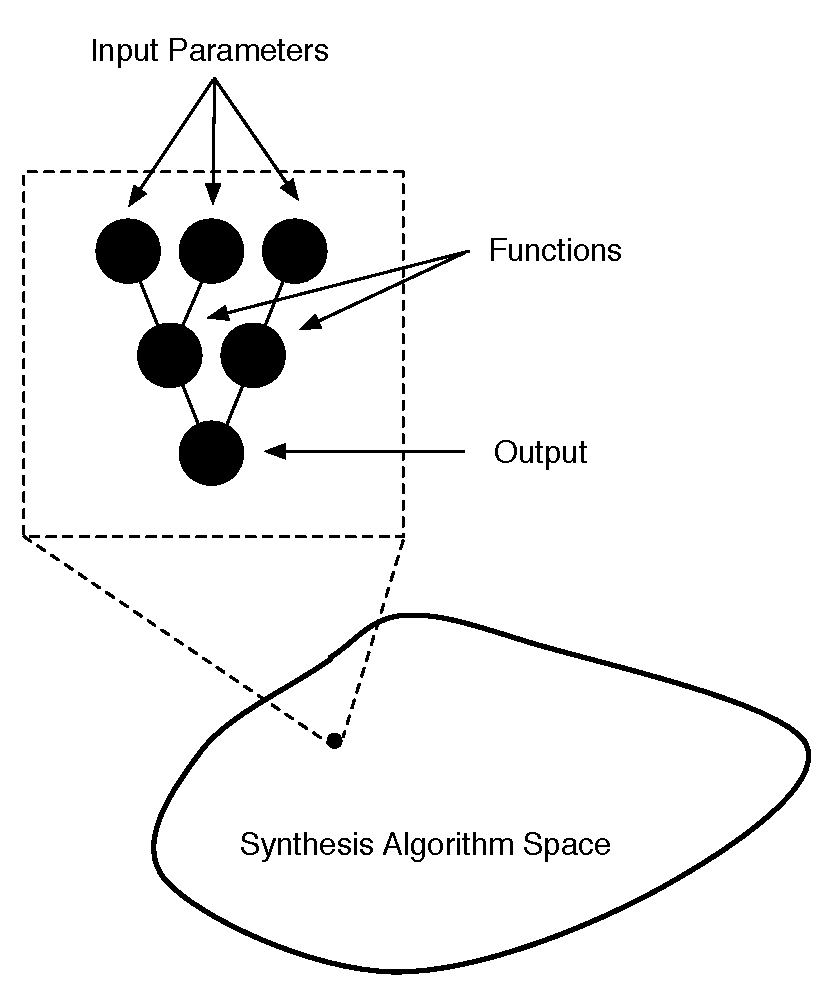
\includegraphics[scale=0.70]{GraphAsPoint}
\caption{The common Genetic Programming (GP) setup, where a point in algorithm space is represented by a tree.}
\end{center}
\end{figure}
There has been relatively little research into genetic programming in the arts compared to the hard sciences (e.g. robotics, circuit design) (Hollady \& Robbins, 2007, p. 1). However, there is no inherent reason why this should be the case. In their paper on human-machine interaction, Moroni, von Zuben, and Manzolli note that ``human-machine interaction in the context of artistic domains [can be] a framework for exploring creativity and producing results that could not be obtained without such interaction'' (2002, p. 185). It is certainly true that a meta-synthesizer would be able to provide a composer with the means to experiment with timbre in ways they would not be able to without it, thus leading them to places of creativity that they would not have been able to explore on their own. However, the first uses of GP in the artistic domain that predated any work on evolving synthesis algorithms were for evolving music-making systems---see (Rowe, 1993); \cite{Spector:1994ij}; (Polito, Daida, \& Bersano-Begey, 1997); (Johanson \& Poli); (Todd \& Werner, 1998); (Costelloe \& Ryan, 2004).

As work in GP was being carried out in the music world, there were also advancements in GP for use in signal processing applications not related to music---see \cite{Sharman:1995bs, Alcazar:1997ve}; (Koza et al., 1997); (Miller, 1998); (Uesaka \& Kawamata, 2000); (Holladay \& Robbins, 2007).

A signal processing application more related to music that has received a lot of attention by GP researchers is automatic feature extraction for various classification tasks. This was predated by GP work on video feature extraction---see (Harris ,1997); (Teller, 1998). 

The first GP system to evolve audio feature extractors was proposed by Conrads, Nordin, and Banzhaf (1998). They used machine-code level GP to extract features for vowel and consonant detection. 

Pachet and Roy also used GP to evolve feature extractors for classification tasks (2007). However, their function set contained much more complicated functions than the work of Conrads et al. Their function set includes a Mel-Frequency Cepstral Coefficient (MFCC) calculation, a Fast Fourier Transform (FFT), and a high-pass filter among others. Their work was recently extended by Kobayashi (2009) and Vatolkin, Theimer, and Rudolph (2009).

Taking into account the Automatic Programming research carried out in both digital signal processing and in music composition over the last fifteen years, one may assume that a good amount of research has also been performed in evolving sound synthesis algorithms. However, this is not the case.

There have been a few studies involving sound synthesis evolution using Interactive-GP (where fitness measurements are provided by test subjects) for timbre exploration---see (Dahlstedt, 2001); (Mandelis \& Husbands); (McDermott, Griffith, \& O'Neill, 2006). However, while each study provides a system that is applicable to any kind of synthesis topology, a fixed topology is chosen for each run of the system. As previously noted, making the user choose a fixed synthesis topology at the beginning of a run can severely limit the regions of timbre space that are even possible to explore. Additionally, using subjective judgements to steer the search requires that the user stay actively involved during the length of the search. A more desirable solution would replace the need for human fitness evaluation with an objective measure that correlates well. In other words, an objective timbre space would have to be developed where distances are semantically meaningful, so that pairwise similarity tests can be performed by the computer.

Wehn was the first researcher to investigate such a system \cite{Wehn:1998bh}. In his work, he uses a basic function set comprised of noise, steady-state sinusoids, triangle and square waves, ramp functions, addition, multiplication, and high, low, and bandpass filters from which to generate more complex algorithms \cite[p. 2]{Wehn:1998bh}. The target sounds that Wehn tests his system with do not vary in time and he does not provide a mechanism by which time-varying sounds can be generated, but as a first step towards our goal, his work is important.

In order to assess fitness, Wehn calculates the Euclidean distance between the amplitude spectra of a target sound and those produced by the synthesizer output \cite[p. 2]{Wehn:1998bh}. Thus, Wehn implicitly assumes a timbre space where each point is represented by the elements of a magnitude spectrum. This is a problematic assumption for many reasons, but perhaps the most important being that such a space is extremely high dimensional and therefore suffers from the ``curse of dimensionality'' (Powell, 2007). Briefly, this states that as the dimensionality of a space increases, the usefulness of distance measurements decrease. In other words, Euclidean distance in a given timbre space will become less meaningful as the space grows in size. Another problem with using a simple Euclidean distance measure, as noted by Vercoe et al., is that ``humans do not measure `noise' or `reduction in quality' of sound in this way'' and so distances will not be semantically meaningful even if the magnitude spectrum were low-dimensional (1998, p. 2).

Wehn places a limit on the size of the resultant synthesis topology, so that its parameter set will be low-dimensional and hopefully more intuitive. However, Wehn's system does not take the other desirable synthesis algorithm features into account (e.g. efficiency, low storage requirements, other aspects of controllability). For example, he does not discuss how a user would gain access nor control the parameters generated for a given target.

Another difficulty with Wehn's system is that his atomic units are extremely low level. Even basic classical synthesis algorithms would require complex combinations of these units and would therefore require significant evolution. Thus, Wehn's input space is needlessly high-dimensional, making search in that space more difficult and time-consuming.

Garcia's research improved on Wehn's both in fitness representation and atomic function set \cite{Garcia:2002cq}. By combining Wehn's function set with more complex atoms (e.g. variable sine and wavetable oscillators, delays, controlled gain filters, time varying filters) Garcia was able to successfully evolve more complex algorithms, capable of generating time-varying timbres. In his results, Garcia demonstrates his system's ability to independently evolve an FM synthesizer  \cite[p. 6]{Garcia:2002cq}. Garcia's system borrows a technique first used by Sharman et al. where topologies are searched for using GP and the optimal parameter set for each topology is separately searched for using simulated annealing (SA) \cite{Sharman:1995bs}. As described by Bensa et al., simulated annealing ``exploits an analogy between the way that metal cools and freezes into a minimum energy crystalline structure and the search for a minimum in a more general system'' (2005, p. 501). Basically, what this means is that simulated annealing allows the search for a global optimum to move into areas of lower fitness (in hope of escaping local optima) with a certain probability that decreases over time (i.e. as the search particle 'cools'). Sharman et al. note that simulated annealing, like GP, has proven useful for finding global optima of multimodal functions (1996, p. 1). However, SA is better suited for smoother and less complex multimodal landscapes and provides a more efficient means of search than GP. Thus, by breaking the synthesis space into a topology space (which is not well understood, but likely rough and multimodal) and a parameter space (which is considered to be smooth and multimodal) one is able to search using separate suitable algorithms for each space. The alternative is to have to choose one search algorithm that may not be optimal for the multi-faceted complexity of the problem at hand. It should be noted that the parameter space will have a different structure for each given topology. Thus, the ``breaking up'' of the synthesis space into two spaces is really more analogous to searching independently over points in a quotient space (re: topology space) and each point's equivalence class (re: parameter space) in that space.

Like Wehn, Garcia also places a limit on the size of the evolved synthesis topologies, thereby reducing the size of the parameter space associated with the optimal topology found \cite[p. 87]{Garcia:2001jw}. However, also like Wehn, he does not incorporate any of the other desirable properties into the search requirements.

The fitness function proposed by Garcia is more advanced than Wehn's. Garcia reduces the dimensionality of the magnitude spectrum-representation that Wehn uses by incorporating perceptually motivated thresholding to allow only certain bin values to be incorporated in the fitness calculation, based on frequency masking \cite[p. 6]{Garcia:2002cq}. While the reduced dimensionality will make Euclidean distances more relevant in the resultant timbre space, it is not clear that these distances will be semantically meaningful, especially if accumulated over time to measure timbre similarity on time scales greater than the FFT frame size used. For example, this representation will consider two time-shifted or slightly time-scaled versions of the same sound to be timbrally dissimilar. Slight nonlinear time warpings or differences in length are also not handled well by this representation. Additionally, the specific choice of perceptual thresholding may be better modeled as a soft threshold as opposed to the hard one used. More advanced perceptually motivated distance metrics can be found in (Riionheimo \& Valimaki, 2003); (Jehan, 2005). Developing an appropriate fitness function is absolutely crucial in designing an efficient GP system (McDermott et al., 2006, p. 3). Without one, the search process can be led in directions that are not relevant to the problem at hand, thus complicating the search process and often ultimately causing its downfall.

Another potential reason why Garcia's system may not be suited for more complex sounds is that his function set is still quite low-level. For example, it would most likely take a long time to evolve something as common as a reverberation algorithm using his function set, but such an algorithm would be quite useful for generating a number of real-world timbres. Holladay and Robbins show that including such domain specific synthesis modules directly into the function set can make the GP system much more powerful (2007, p. 4). The idea of incorporating such modules into the function set along with low-level topological atoms was first proposed by Koza and has been used widely in GP research (1992).

The above review of using GP to automatically generate synthesis algorithms given a target timbre shows that there is still much research to be done. Specifically, there are three areas of investigation that will make these systems more powerful, which happen to be the three areas that are most responsible for the successfulness of all GP systems: an appropriate primitive/function set, a well-designed fitness function, and heuristics to refine the search space and thus speed-up the search. In this problem-domain, this translates to specifying an atomic set of topologies that allow for efficient search (by not being too low-level) without preventing optimal solutions (by not being too high-level), an appropriate measure of timbral similarity (re: a better fitness function), and a more thorough treatment of ways in which to restrict the search based on the desirable features of an optimal synthesis algorithm. 

\section{Audio-Implementation Systems}

Audio-implementation systems, such as Max, CSound, Supercollider, and ChucK, provide a more technically-oriented composer with the ability to experiment with sound synthesis and audio effect design. Many of the goals these software systems try to meet are in line with the goals of the desired meta-synthesis system we have previously described (Moreno, 2005). In fact, these software solutions can be viewed as meta-synthesis systems that place the onus on the user to search for a specific timbre by combining the atomic building blocks available to them. 

A main goal of such systems is to abstract away the low-level audio programming that would not be beneficial to a composer interested in timbral exploration (Moreno, 2005, p. 1). This has to be balanced however with the goal of providing a user with functional elements that are low-level enough so that they may be combined into topologies able to produce any timbre in a reasonably efficient manner (Moreno, 2005, p. 1). Thus, these systems typically provide functions that are both low-level and useful in many signal processing applications (e.g. sample addition) and high-level modules that would require complex design using only the lower-level functions, like the FFT or reverberation. The balance of the above goals is the exact same balance we face when choosing an appropriate function set for GP to evolve synthesis algorithms. Therefore, we will rely on the many years of development, user-feedback, and re-development of these systems to determine the appropriate level of abstraction necessary for an efficient GP search. If fact, Johnson picked up on this years ago in discussing a possible system by which synthesis algorithms may be evolved by GAs. In noting the suitability of Max as such a system he writes, �it would be easy to fit the evolution of Max patches into this framework� \cite[p. 6]{Johnson:1998sh}.

\section{Timbral Similarity}

In order to define a better objective fitness function to measure the subjective nature of timbral similarity, we can look to a large body of work dedicated to the subject. 

The reliance of timbre similarity on timbral evolution trajectories is well-supported and fits in line with an objective timbre space representation we have adopted. Toiviainen et al. note that a major component of the perception of timbre and measuring timbral similarity is the time-varying spectral envelope of sound (1998, p.225). This is further supported by Caclin et al. and also separately noted by Ciglar in more recent studies (Caclin et al., 2005, p. 1); \cite[p. 4]{Ciglar:2009uf}. 

Therefore, appropriate timbre similarity models will measure similarities (re: sematically relevant distances) between trajectories of perceptually relevant timbre features. Using the results from the subjective timbre space literature, a number of researchers interested in Music Information Retrieval (MIR) have developed such models.

The MIR community has investigated music similarity on a number of different levels. Some research has been aimed at rhythmic similarity (Paulus \& Klapuri, 2002), other at harmonic similarity (de Haas, Veltkamp, \& Wiering, 2008), and, more recently, structural similarity \cite{Bello:NoRead}. However, timbre similarity has been a main focal point in the community for a number of years. The quest for an appropriate timbral similarity measure has also seen the development of a number of different timbre features for use within similarity models. 

Early work in timbre similarity was aimed at classifying instruments, which is quite appropriate given that work on subjective timbre spaces could alternatively be seen as generating spaces with good discrimination properties for instruments (Loureiro, de Paula, \& Yehia, 2000); (Park, 2004); (Timoney, Lysaght, Mac Manus, \& Schwarzbacher, 2004); (Zhang \& Ras, 2006). This research takes the viewpoint that timbre is related to its sound-production mechanism and therefore develops models that will assign similar timbre to all sounds generated by the same instrument. Many of the features used in the literature are designed specifically for monophonic instrument sounds and do not apply to polyphonic mixtures or more complex timbral evolution \cite[p. 6]{Ciglar:2009uf}. For example, these include features that measure the temporal progression of an instrument's harmonic partials, features related specifically to the attack, sustain, and release portions of a note, as well as strength relations between odd/even partials (Timoney et al., 2004, p. 182). In order to develop a more general timbre feature representation, applicable to both monophonic and polyphonic sounds, the community focused on a more complex problem: genre recognition.

It is important to note that genre recognition systems are primarily interested with timbre on a global time scale (i.e. over an entire song). It is because of this large body of research that Johnson and Gounaropoulos make a distinction between local and global timbre \cite{Johnson:2006pi}. However, even though genre recognition systems are not necessarily interested in local timbral evolution (as we are), genre recognition research requires a representation of timbre for complex polyphonic signals, and thus a lot can be learned from such work.

Aucouturier and Pachet were two of the first researchers to investigate a system for genre classification \cite{Aucouturier:2002gf}. The basic idea in genre recognition is that each genre has unique timbral properties on the global scale and therefore by measuring these properties given an unlabeled song, one is able to automatically assign it a genre. Aucouturier and Pachet borrow a feature set from the speech community known as Mel-Frequency Cepstral Coefficients (MFCCs) that have now become ubiquitous as timbre features \cite[p. 1]{Aucouturier:2002gf}. In speech processing research, ``MFCCs were developed to model the spectral envelope while suppressing the fundamental frequency'' \cite[p. 1]{Jensen:2006dw}. Thus, they are often considered to be a compact representation of the spectral envelope (a typical feature included in the additive definition of timbre) divorced from pitch (a property from the negative definition of timbre). Aucouturier and Pachet model the probability density of all of the MFCCs from a genre using a Gaussian Mixture Model (GMM), which is simply a multimodal (and often multivariate) distribution composed of Gaussian components (see Figure 2.21). In order to determine the genre of a set of test samples, MFCCs are extracted and their likelihood under each genre model is calculated. The most likely genre is assigned to the set of test samples \cite[p. 2]{Aucouturier:2002gf}.
\\
\begin{figure}[h!]
\begin{center}
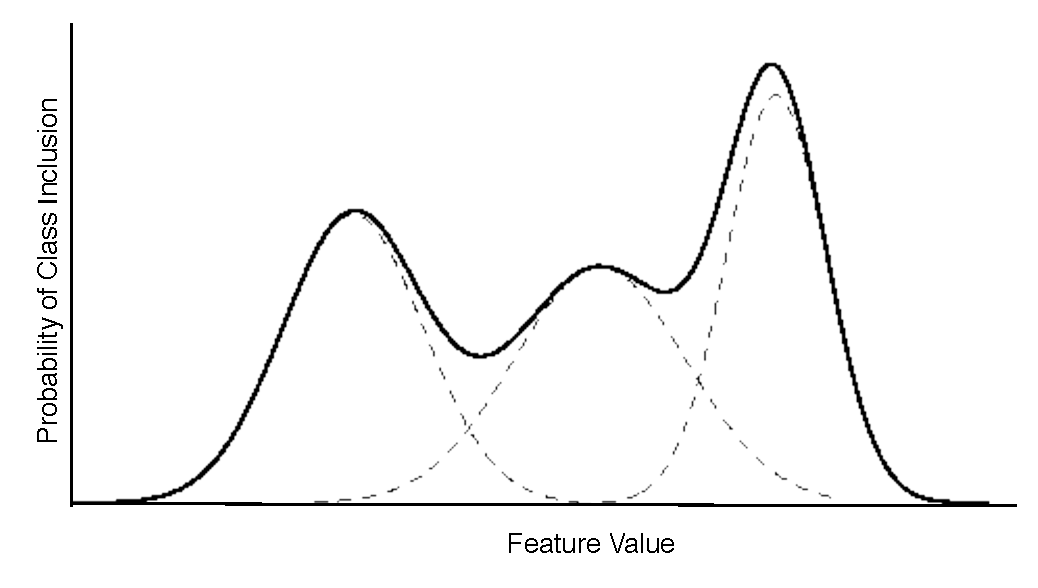
\includegraphics[scale=0.70]{GMM}
\caption{An example of a univariate Gaussian Mixture Model (GMM) taken from (Schwardt, 2005).}
\end{center}
\end{figure}
Following the work of Aucouturier and Pachet, Pampalk also modeled the timbral content of music with GMMs of MFCCs in his dissertation on sound similarity \cite{Pampalk:2006pr}. However, instead of classifying songs by genre, Pampalk was primarily interested in calculating pairwise similarity between songs. He separately modeled each song with a GMM and calculated the similarity between GMMs using two common distance metrics for probability distributions: Kullback-Leibler (KL) Divergence and Earth Mover's Distance (EMD) \cite[p. 26]{Pampalk:2006pr}. Roughly speaking, KL Divergence (also known as relative entropy in Information Theory literature) is a measure of how well one distribution approximates another (and is therefore not symmetric) while the EMD is a measure of how ``much'' one would have to change the shape of one distribution in order for it to look like the other. Determining whether such models are appropriate for pairwise similarity is a difficult task. In order to properly measure the accuracy of a given model, a sound similarity ground truth must be designated.

As noted by Seyerlehner and Widmer,``ideally, a content-based audio similarity metric should approximate the ill-defined `sounds-like' related for songs'' (2008, p. 1). However, Logan, Ellis, and Berenzweig point out that similarity ratings can vary ``not only across users, but across time, according to mood and according to context'' (2003, p. 1). This is verfied by Pampalk et al. \cite[p. 6]{Pampalk:2008xz}. By testing enough users, one may be able to form a meaningful consensus, but user-testing is expensive (both in time and money) and alternate ground truth data is often desired. Therefore, some other labeling is usually accepted (e.g. genre), whether it is provided by experts or by clustering user-provided tags (p. 2). The extent to which this data approximates ``sounds-like'' is unclear. An even more important question, however, is whether ``sounds-like'' on the global timescale is truly a measure of similarity between two songs. Many other factors could play a role (e.g. lyrical content, popularity). In Jensen's dissertation, he writes that:

%\linespread{1}
\selectfont
\begin{quote} The inherent problem, that genres are a cultural as much as a musical phenomenon, persists...in our opinion, genre classification as a research topic in signal processing should be abandoned in favor of specialized tests that directly evaluate the improvements of proposed algorithms. The short time features that only capture timbre similarity, or methods using source separation, could e.g. be tested in a polyphonic identification setup that much better shows the capability of the algorithms \cite[p. 11]{Jensen:2009ta}.
\end{quote}
%\linespread{1.7}
\selectfont

Aucouturier and Pachet do note in their 2003 paper that in studying genre recognition, ``the problem of the actual perception of timbre is not addressed by current methods'' \cite{Aucouturier:2003gs}[p. 16]. However, this facet of MIR continued to be synonymous with timbre similarity for a number of years and was used to measure the accuracy of systems like Pampalk's \cite{Pampalk:2006pr}. The fact that genre classification results did not see any marked improvements over that time was actually a good thing for timbre research, because it stimulated a wide variety of approaches towards finding better timbre features and incorporating them into better similarity models.

For example, Meng, Ahrendt, and Larsen attempt to improve genre classification results by integrating short-time timbre features, on the order of 30ms, into medium (on the order of 740ms) and long-term (on the order of 9.62s) timbre features in order to better model the temporal evolution of timbre on longer time scales \cite[p. 498]{Meng:2005fx}. The authors suggest calculating simple statistics, using dynamic PCA (where features are stacked over the desired time horizon and PCA is used to reduce the dimensionality of the resultant feature vector), and modeling the time-varying properties of a sequence of MFCCs by calculating the power spectrum of each (p. 498). They found best results using these latter features, which they called filterbank coefficient (FC) features. These features are able to capture MFCC modulations over a number of modulation rates (with a resolution determined by the length of the time horizon). 

Heise et al. use similar features to Meng et al.�s FCs (2009).
Instead of calculating the power spectrum of each MFCC over a specified time window, they compute a discrete cosine transform (DCT), which decorrelates and compresses the MFCCs spectral data in the first few bins while retaining the characteristics of its shape. The result is a MFCC spectral matrix where each row represents a different MFCC. The authors reduce the dimensionality of this feature matrix by either throwing away the high MFCCs (retaining good MFCC spectral resolution, but smoothing out the signal�s spectral envelope), or by throwing out the last columns (retaining good signal-spectral-envelope resolution, but smoothing out the MFCC spectral resolution) (2009, p. 3).

Pampalk, Flexer, and Widmer develop fluctuation pattern (FP) features that are derived from a perceptually transformed spectrogram. Again, like Meng et al. and Heise et al., these authors incorporate the temporal evolution of the features by taking the FFT over each band in their perceptual spectrogram \cite[p. 4]{Pampalk:2005ix}. They find that incorporating these features do not improve genre classification performance, but again, this does not necessarily mean that they are not modeling the timbre more accurately \cite[p. 8]{Pampalk:2005ix}.

Incorporating the temporal evolution of timbral features over some time horizon using the FFT of each feature over that horizon is an interesting idea that requires more research outside of the domain of genre recognition so that it may be fairly evaluated.

A number of other features have been used alongside MFCCs (on the same time scale) in hopes that additional timbre information will be contained in some or all of them. Most often, due to the curse of dimensionality, feature selection methods are used to find those features that boost performance the most, while filtering out those that provide marginal contribution. 

Allamanche, Herre, Hellmuth, Kastner and Ertel start with a set of features including normalized loudness, delta log-loudness, spectral flatness measure, spectral crest factor, real cepstral coefficients, spectral tilt, spectral sharpness, and zero crossing rate along with MFCCs (2002). For feature selection, they perform a greedy search by first finding the single feature that provides best classification, then adding to it the feature that helps it perform best, etc.

McDermott et al. investigate 40 different features commonly used in MIR research and eliminate features based on their redundancy in the presence of others (2005, p. 1). The authors split these features into six groups, based on the type of feature---time domain, Fourier-transform domain, partial domain, trajectory, periodic, or statistical---and find that features within the same group tend to be redundant in the presence of others in that group, an un-alarming result (p. 6).

Kobayashi uses evolutionary algorithms to breed linear combinations of features that provide the best classification performance (2009). His system is based around instrument recognition, but the principle would be valid for any type of classification. As opposed to Pachet and Roy's work (2007) on using GP to breed single discriminatory feature, Kobayashi starts with a general feature set, able to extract information from scalars, vectors, and/or matrices, and evolves the best linear combination of discriminatory features.

Evolving features or proper combinations of features is a natural direction for feature selection. Instead of relying on hand-crafted feature sets and information-theoretic assumptions about what makes a feature ``useful'', these methods evolve functions that well-suited for their problem-domain. A downside to such methods, however, is that one must evolve a new feature or set of features for each problem.

Another option as opposed to feature selection for timbral similarity is intelligent feature combination, as proposed by Fu, Lu, Ting, and Zhang (2009). As opposed to selecting a subset of features that improves classification over the entire feature set, feature combination attempts to combine all features in a way that  improves performance over any single feature vector.

Seyerlehner et al. take a subtractive approach to feature �selection� by searching for feature vectors that are not perceptually relevant (e.g. silence) and filtering them out (2009). They note that in modeling a feature vector sequence containing some silent frames using a GMM, the distribution will contain a peak at the silent location in space. Thus, if another feature vector sequence�s likelihood is computed and it also has silent frames, then a non-negligible likelihood will result no matter how different the non-silent frames are from one another between the two sequences. The authors find that these low energy frames thus contribute greatly to the measure of similarity, which is undesirable (2009, p. 3).

While feature combination/selection methods expand the space of feature possibilities by looking not only at hand-crafted features, but also any linear combinations of them, there is a strong reliance on the assumption that all important timbal information is contained in this hand-crafted feature space and that a combination of hand-crafted features exists that not only contains all timbal information, but also that contains little information about any other musical dimensions (i.e. the feature combination has little noise). A more direct approach to learning low-noise timbal features is to not limit the feature space to only contain linear combinations of hand-crafted features, but instead to allow more fundamental building blocks from which to generate timbal features.

Humphrey, Glennon, and Bello's \cite{Humphrey:2000th} work directly learns timbre features using machine learning architectures known as Convolutional Neural Networks (CNNs). Their approach learns a nonlinear projection from basic high-dimensional spectral representations of audio to a low-dimensional space where distances are semantically meaningful in the sense that two points that are close together will be considered timbrally similar and two points that are far apart, dissimilar. Their work focuses on the instrument recognition task and uses an iterative learning process to ensure that two sounds that are transformed by the same projection that come from the same instrument resolve down to points close in timbre space. The nonlinear projection imposed by the resultant CNN can be viewed as feature extraction, where projected points reside in a feature space that is representative of timbre.

Determining the most appropriate objective timbre representation is still an unsolved problem. While MFCCs are ubiquitous as timbre features, BOF approaches (requiring feature selection or combination) and early fusion techniques have potential to improve upon this representation. However, one still may find the best timbre representation comes from its negative definition (by removing pitch and loudness) rather than its additive definition, which is equally flawed. 

Humphrey, Glennon, and Bello's work relies on the assumption that, given a set of instruments, more often than not timbrally similar sounds produced within that set are likely to come from the same instrument. While there may be cases where this is not true, given a wide range of content, we believe this assumption to be more valid than that which underlies genre recognition and therefore will utilize this feature learning method in our system.

As opposed to trying to improve the timbre \emph{representation} for a boost in genre classification performance, there has also been a push in the literature to improve the metrics used in timbre similarity engines, rather than relying on the typical calculation of KL-Divergence between GMMs of timbre features, as used by Pampalk \cite{Pampalk:2006pr}. The primary weakness of this often-used metric is that it ignores information about the temporal evolution of timbre. This information is thrown away when modeling the observed series of timbre feature vectors with a GMM probability distribution. While previously discussed research has attempted to incorporate temporal information into the features themselves (this is known as early fusion), other research has focused on incorporating temporal information into the classifier (known as late fusion) \cite[p. 500]{Meng:2005fx}.

For example, Flexer, Pampalk, and Widmer model similarity using a Hidden Markov Model (HMM) instead of a GMM \cite{Flexer:2005sw}. In describing their decision, they note that �aspects like spectral fluctuation, attack or decay of an event cannot be modeled without respecting the temporal order of the audio signals�, which the GMM does not do (2005, p. 1).HMMs allow one to model time-varying timbral data using probability density functions representing locally stationary timbre and transition probabilities between those stable states (2005, p. 2). Thus, the temporal variation in timbre is directly incorporated into the model. However, in most implementations, first-order HMMs are used (due to their computational efficiency in comparison to higher order models), which retain only the temporal information regarding how neighboring feature vectors are ordered. This combined with the fact that this is a probabilistic mode, means that some information about the temporal evolution is lost. However, one would expect this to result in a much more adept model at calculating timbral similarity. Flexer et al. found, however, that this model did not achieve significant gains in genre classification performance (p. 5). As stated, this does not necessarily mean that HMMs do not provide any significant gains in generating semantically meaningful timbre distance measurements.

Jehan, in his dissertation, calculates similarity between perceptually processed spectral data using dynamic time warping (DTW) (2005, p. 70). By aligning the feature data between two feature vector sequences, one is able to account for slight time warpings and/or shifts between the sequences, allowing for a simple Euclidean distance calculation between aligned sequence vectors in order to calculate similarity. Jehan also incorporates the importance of the attack towards timbre perception directly into the DTW algorithm by dynamically weighing the path with a half-raised cosine function (p. 71). While DTW retains virtually all of the temporal evolution information of a timbre feature sequence, it has an undesirable time-complexity. However, recently an O(N) variant of DTW, called FastDTW, that restricts the warp path based on reasonable assumptions has been developed (Salvador \& Chan, 2004).

Late fusion similarity models like the HMM or DTW are also a step in the right direction away from GMMs. However, other models should be investigated as well. As previously noted, low-order HMMs only retain short-time temporal information, and, while the DTW retains virtually all of the temporal evolution information in a sequence of timbre features, there may be examples where slight time warping or shifting is not enough to align two sequences that are semantically similar. For example, if two sound files contain the same distinct, repetitive timbral gesture, but one file contains a larger number of repetitions than the other, DTW will be unable to globally align them and therefore will consider them timbrally dissimilar. A more appropriate comparison in this case may be analogous to a continuous space sequence similarity measure.

Our approach (as will be laid out in detail later) follows this train of thought by modeling timbre similarity over a curve in an objective timbre space as determining the similarity between sequences of atomic timbre subsequences. Our approach provides similar results to direct Euclidean distance between feature vectors if the sounds compared are time aligned and not time warped and similar results to DTW if time warped and/or not time aligned, but also provides an appropriate similarity measure for when either a different number of repetitions are present in the sounds being compared, when timbre subsequences are re-arranged, or when two sounds' timbre curves only partially overlap - after some alignment and local warping - but diverge otherwise.

Recent research into timbre similarity already presents a wealth of information that will can improve upon the fitness calculations used thusfar in research involving the evolution of synthesis algorithms. However, we believe our approaches to both timbre feature extraction and timbre similarity measurement represent state-of-the-art techniques, which provide the best chance of evolving synthesis algorithms that accurately model any target sound with time-varying timbre.

\section{State-of-the-Art Genetic Programming}

The main deterrent to using any GA variant is that, in comparison to other search techniques, it is a very slow search process. Todd and Werner note that ``the main reason for this sometimes-glacial pace is that...evolution builds systems through the gradual accrual of beneficial bits and pieces, rather than through systematic design or rapid learning from the environment'' (1998, p. 5). Another reason for GAs inefficiency is the fitness calculation bottleneck, as discussed by Riionheimo and Valimaki (2003, p.10). Typically most of the search time is spent calculating the fitness of each individual. If a fitness calculation is not needed (i.e. if there is a known mathematical relationship between the input parameter space and the output space) then the search would be sped up tremendously, however, in such cases, analytical solutions are often available.

Due to its inefficiency, GAs are often used only as a last resort in search problems. However, for problems that are not well understood or which are known to have complex multimodal fitness landscapes (e.g. Automatic Programming), they often provide the only solution. Much research has been carried out to find ways in which to increase the efficiency of search. Most often, these methods are aimed at restricting the search space using a set of heuristics that include both problem-domain dependent and independent knowledge. The problem-domain independent methods designed to restrict the search space and/or improve the search ``quality'' of the GP system influence every part of its structural design. We apply the term heuristics both to architecture decisions as well as limitations imposed on the architecture because, as pointed out by Vanneschi, �the art of choosing an appropriate representation and an appropriate set of operators is often a matter of experience and intuition� and therefore all design choices are either based on personal or historical trial-and-error (2004, p. 6).

A number of GP enhancements have already been described. For example, the GP/SA architecture used both by Alcazar and Sharman \cite{Alcazar:1996la} as well as Garcia \cite{Garcia:2002cq} is a way to improve the parameter search using simulated annealing, which is likely better suited for its fitness landscape. Also, incorporating higher-level modules into the function set along with low-level building blocks has been shown to make GP more powerful in various problems (Koza et al., 1997). 

Another enhancement to the proposed system is the ability for basic function elements to handle vectors as a native data type. The inability to, for example multiply a stream of numbers by a scalar, is cited by Holladay and Robbins as a major deterrent to Automatic Programming systems that require such operations (2007, p. 1). If such simple operations on vectors are not possible, then the loop structures underlying their execution would have to be evolved separately.

When applying methods to restrict the search space, one must be careful not to restrict the space within a region that does \emph{not} include the optimal solution. A popular way to naturally restrict the search space (without the possibility of omitting the optimal solution) is to use strongly-typed GP (STGP), which enforces data type constraints, so that only syntactically correct structures are searched (Harris, 1997); (Vanneschi, 2004); (Pachet \& Roy, 2007). Basic GP does not enforce such rules and so it is possible that topologies will be searched that are invalid. Enforcing data type constraints during search is a simple way to disregard such topologies and make the search much more efficient. An example of a syntactically-correct Max patch and a syntactically-incorrect Max patch are shown in figure 22.
\\
\begin{figure}[h!]
\begin{center}
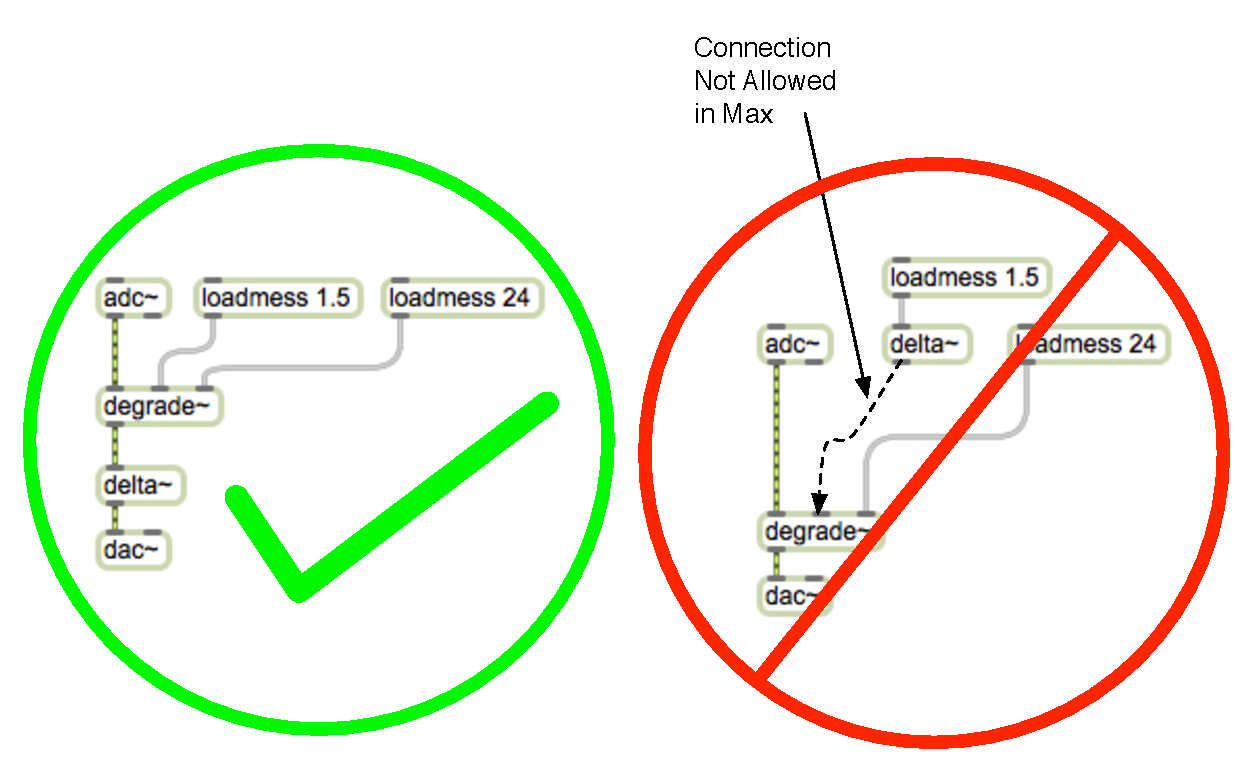
\includegraphics[scale=0.70]{SyntacticCorrectness}
\caption{A syntactically correct Max patch that would be included in a STGP search space and a syntactically incorrect one that would not be (due to the labeled disallowed connection).}
\end{center}
\end{figure}
One of the major problems that GP systems face, efficiency-wise, is code bloat. Bloat, as defined in da Silva's dissertation, is `an excess code growth without a corresponding improvement in fitness' (p. 2008, p. 2). There are a number of theories as to why bloat occurs in GP systems, but da Silva notes that strong evidence supports that bloat is a side-effect of the search for higher fitness and therefore intricately linked to GP search (p. 9). The problem is analogous to the overfitting problem in machine learning. da Silva writes that `programs tend to grow until they fit the fitness data perfectly' (p. 9).

da Silva separates bloat control methods into four categories based on where in the search process control is applied: evaluation, selection, breeding, and survival (2008, p. 11). In evaluation methods, the desire for parsimony is directly incorporated into the fitness function (p. 11). Selection methods apply rules that favor parsimonious solutions when selecting individuals for breeding (p. 12). Breeding methods introduce genetic operators that are designed specifically to restrict code growth (p. 12). Finally, survival methods only allow candidates from one generation to move on to the next if they meet certain size requirements (p. 12). 

In da Silva's dissertation, he rigorously compares the most popular methods in each category using a number of test problems, differing in complexity, representation, and domain. da Silva finds that a combination of Dynamic Maximum Tree Depth (DMTD) and dynamic Resource-Limited GP (dRLGP) outperformed all other methods consistently (2008, p. 86). 

DMTD is an extension of the static-depth limits (SMTDs) imposed by both Wehn \cite{Wehn:1998bh} and Garcia  \cite{Garcia:2002cq} in their research to restrict the size of the evolved synthesis topology and, more importantly from a user perspective, the parameter set. The difference between DMTD and SMTD, as the names imply, is that DMTD imposes a depth limit that changes throughout the search process. Specifically, DMTD works by first setting an initial depth limit when generating the first population. A new individual that breaks this limit will be replaced by its parent, unless it is the most fit individual so far in the run. In this case, the dynamic limit is adjusted to match this length and breeding continues with the new limit until another most-fit-individual breaks it (da Silva, 2008, p. 17).

dRLGP is a variant of Resource-Limited GP (RLGP). In RLGP, a single resource limit is imposed on the entire GP population (da Silva, 2008, p. 21). Every topology node and parameter node in a population is considered a resource. The limiting of such ``resources'' models the limiting of natural resources available to a given biological population, considered a main component of evolution (p. 21). The process works as follows: offspring of a population are sorted by fitness, followed by their parents; programs in this list are given resources going from most fit to least fit; if an individual needs more resources than are available, it is passed over and not allowed into the next population. dRLGP adjusts the size of the resource limit if the mean population fitness is greater than the mean fitness of the best population in the run thusfar (p. 22). 

Imposing such limits will pressure the system into developing parsimonious solutions (which is good for synthesis algorithm controllability and efficiency) while severely restricting the search space (which makes the search process itself more efficient). A further benefit of using these limits to control code bloat as opposed to evaluation, selection, or breeding methods, is that they are parameterless and can be used with any selection method (da Silva, 2008, p. 97)

Another solution that is commonly used to improve the efficiency of the search (which also has added benefits related to the quality of the evolved algorithms) is called the ``Parallel and Distributed Genetic Programming'' (PADGP) technique based on parallelizing the GP search process (Vanneschi, 2004, p. 13). In PADGP, the search divides the initial population into a number of subpopulations that evolve independently, with frequent exchange of individuals between subpopulations (p. 174). The only communication between subpopulations occurs when the exchange of individuals is necessary. The ability to evolve subpopulations independently allows one to parallelize the search process, speeding up the search tremendously (p. 173). However, the true benefit of the island model is that it prevents another major problem of GP, premature convergence (p. 15).

Vanneschi writes that ``premature convergence, both from the view of the variety of the fitness values and of syntactic structures, is an experimental evidence in almost all the GP applications'' (2004, p. 15). Convergence is ``used to describe the state of affairs when the population becomes largely homogenous, consisting largely of variations on a single style of solution'' (Vanneschi, 2004, p. 26). When this happens prematurely, the system will output a sub-optimal solution. Crossover, one of the two basic genetic operators used in GP (along with Mutation) allows propagation of small blocks of code that were useful in previous populations (or, at the very least, part of useful algorithms) into future populations. While this is the main mechanism for code re-use during the GP search, it ``tends to encourage a uniformity in building solutions and can contribute to convergence problems'' \cite[p. 30]{Wehn:1998bh}. Vanneschi shows, via rigorous testing, that the PADGP is a natural way of maintaining diversity, and thus preventing premature convergence, inside GP populations (p. 213). He compares the effects of this model to a number of other methods designed specifically to limit premature convergence and finds that it works as well or better than these other methods (p. 221). He notes that additionally ``one advantage of multiple populations as means for maintaining diversity is that, in contrast to the clever methods above, diversity is maintained `for free', so to speak, without any particular algorithmic device beyond the simple communication among islands'' (p. 213). Vanneschi also suggests that using the island model has a better chance at finding global optima in multimodal landscapes due to the division of the space into a number of mini-parallel searches, as opposed to a singular parallel search over the entire space (p. 192). He writes that this has the effect of speeding up the search as well and that parallel GP would provide for a more efficient search even if implemented on a single processor (p. 230).

In order to further restrict the search space, one can also develop heuristics appropriate for the specific problem-domain. A common example is restricting the possible parameter values by discretizing a finite range, as suggested in (Riionheimo \& Valimaki, 2003, p. 6). This process provides the possibility of omitting the optimal solution from search and so restriction on parameter values should not be too severe. Riionheimo and Valimaki suggest attempting to limit the range of parameters so that they are able to just cover all possible musical ``tones/' and discretize with a resolution that is below the discrimination threshold (2003, p. 6) However, determining such ranges and resolutions is a complex process. Martens and Marui found that, at least for vibrato flange and stereo chorus, the useful ranges of parameters were roughly the same (p. 4). However, a more detailed study by McDermott et al. show that, in general, ``useful'' parameter ranges vary for different synthesis topologies and therefore must be found for each new topology one is presented with (2005, p. 5). Therefore, it is important to err on the side of caution when specifying such limits. One can also place limits on the functions used in each run. However, in general, ``the function and terminal sets should be chosen so as to verify the requirements of closure and sufficiency'', so restricting the function set can be as dangerous as limiting parameter ranges (Vanneschi, 2004, p. 22). 

A method used to improve the ability of GP to find optimal solutions that is directed at the fitness function definition is presented by McDermott et al. (2006). By defining a set of ``increasingly discriminating fitness functions (IFFs)'' one is able to reward minor progress at each stage of the search in a way not possible using a statically defined fitness function (p. 15). The basic idea is to reshape the fitness landscape throughout the search so that the optimal solution becomes more and more difficult to obtain as the search progresses. Early on in the search when individuals in the population perform poorly, the grading mechanism is more lenient and differences between extremely poor solutions and only slightly better solutions is magnified. As the mean fitness over the population increases, the fitness function can grow to become more and more difficult to satisfy. In effect, one is manually evolving the fitness function along with the population.

It is our belief that the research discussed above along with improved measures of timbral similarity can combine to push synthesis topology evolution past a point of only being able to generate simple, ``toy-example'' topologies. By utilizing a meta-synthesis software environment like Max, that was specifically designed to provide synthesis building blocks with the exact level of abstraction required by an efficient GP system, we expect our results to contribute greatly to this area of research.
\newpage
\vspace*{\QuarterPage}
\chapter{Methods} % * suppresses heading numbers	
\section{System Design}
\subsection{Languages and Interoperability}
By relying on the many years of development, user-feedback, and re-development of commercial audio-implementation systems to provide the appropriate level of abstraction necessary for an efficient GP search (as discussed in the Prior Work above), we have decided to apply GP directly within one of these audio-implementation systems. While those previously listed would all be good candidates for evolving synthesis algorithms, Max (developed by \emph{Cycling '74}) is chosen because, as pointed out by Lazzarini, ``MaxMSP and its variants have lately become the most used of these systems, because of their user-friendliness'' (2004, p. 356). Lazzarini's statements have two implications. First, due to Max's popularity, the resultant algorithms (i.e. Max patches) output from our system will be available to more composers. Second, due to Max's ease of use, the algorithms will automatically be accompanied by interfaces for timbre exploration that are accessible to the non-technically oriented composer, whom this research will benefit most.

While it would be possible to design the entire system in Max by utilizing either Java via the \emph{mxj} object or JavaScript via the \emph{js} object for the implementation of the GP framework, the timbre feature extraction, and the timbre similarity calculation code, we have decided to use Python for the 'heavy lifting' instead. The main reason for this choice is that Python has an extensive set of third-party libraries developed for it in the domains of machine learning, artificial intelligence, music information retrieval, etc. that allow for rapid development of all the necessary code used for timbre extraction and similarity calculations. It also has popular linear algebra libraries (numpy, scipy) and a popular and easy-to-use graphing framework (matplotlib) that may be utilized throughout the codebase to simplify calculations and produce figures exhibiting our experimental results.

Therefore, we have implemented all genetic programming code, which includes both the fitness function calculation and the genetic operator applications that follow in Python. This means that the only processing required of Max is the actual patch creation (within the Max environment) and the signal processing that follows.

The problem with choosing a language that does not directly interface with Max, which is the case with Python, is that a translation layer must be inserted between Max and the chosen language so that they can communicate appropriately. Given the tasks assigned to Python and those assigned to Max, one may observe that this communication can be described as follows:
\begin{enumerate}
\item Python communicates to Max what patch to generate, including all objects and connections between object inlets and outlets. 
\item Max communicates to Python the `results' of its signal processing through the generated patch.
\end{enumerate}
The first item is handled using a JavaScript translation layer, where Python translates its internal representation of a Max patch into JavaScript code, which the Max js object immediately runs to generate the desired Max patch (see Figure 3.1). 
\begin{figure}[h!]
\begin{center}
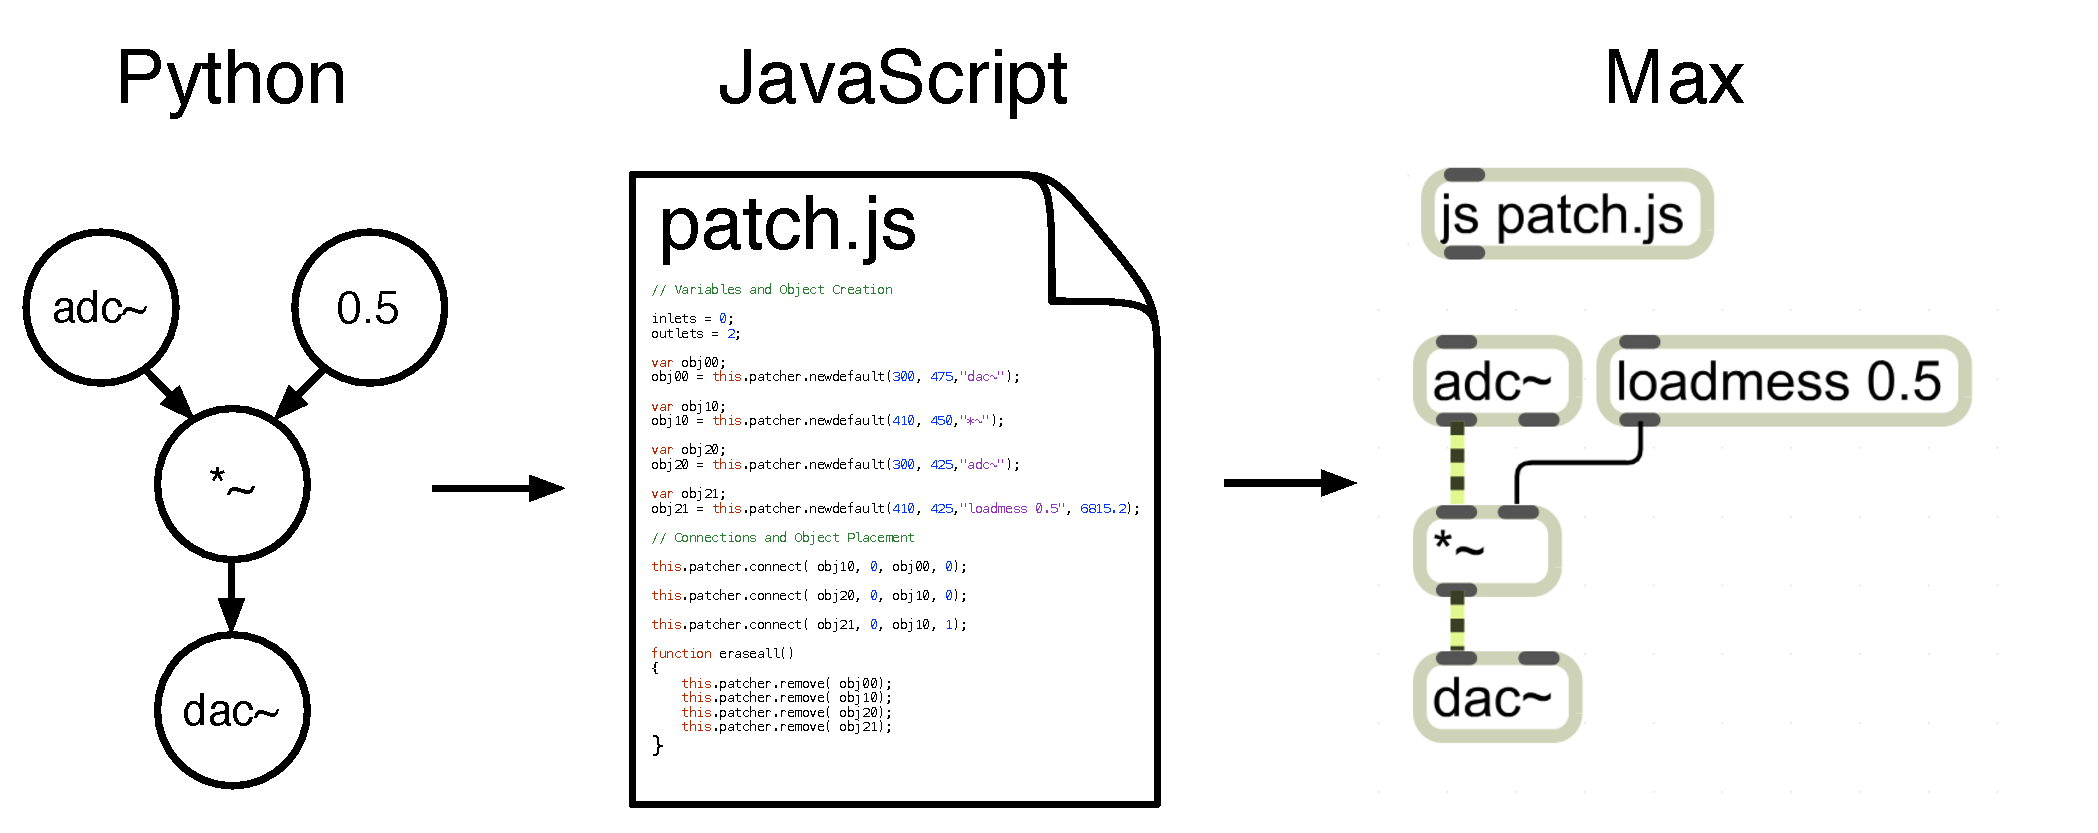
\includegraphics[scale=0.4]{JSTranslation}
\caption[Generating a Max patch given a parse-tree]{Translation of a Python `MaxPatch' into an equivalent patch in Max via JavaScript.}
\end{center}
\end{figure}
\\
The second item is handled by requiring Max to write the audio at the output of a given Max patch to a file, which is then read  by Python and used for the timbre feature calculation (see Figure 3.2).
\begin{figure}[h!]
\begin{center}
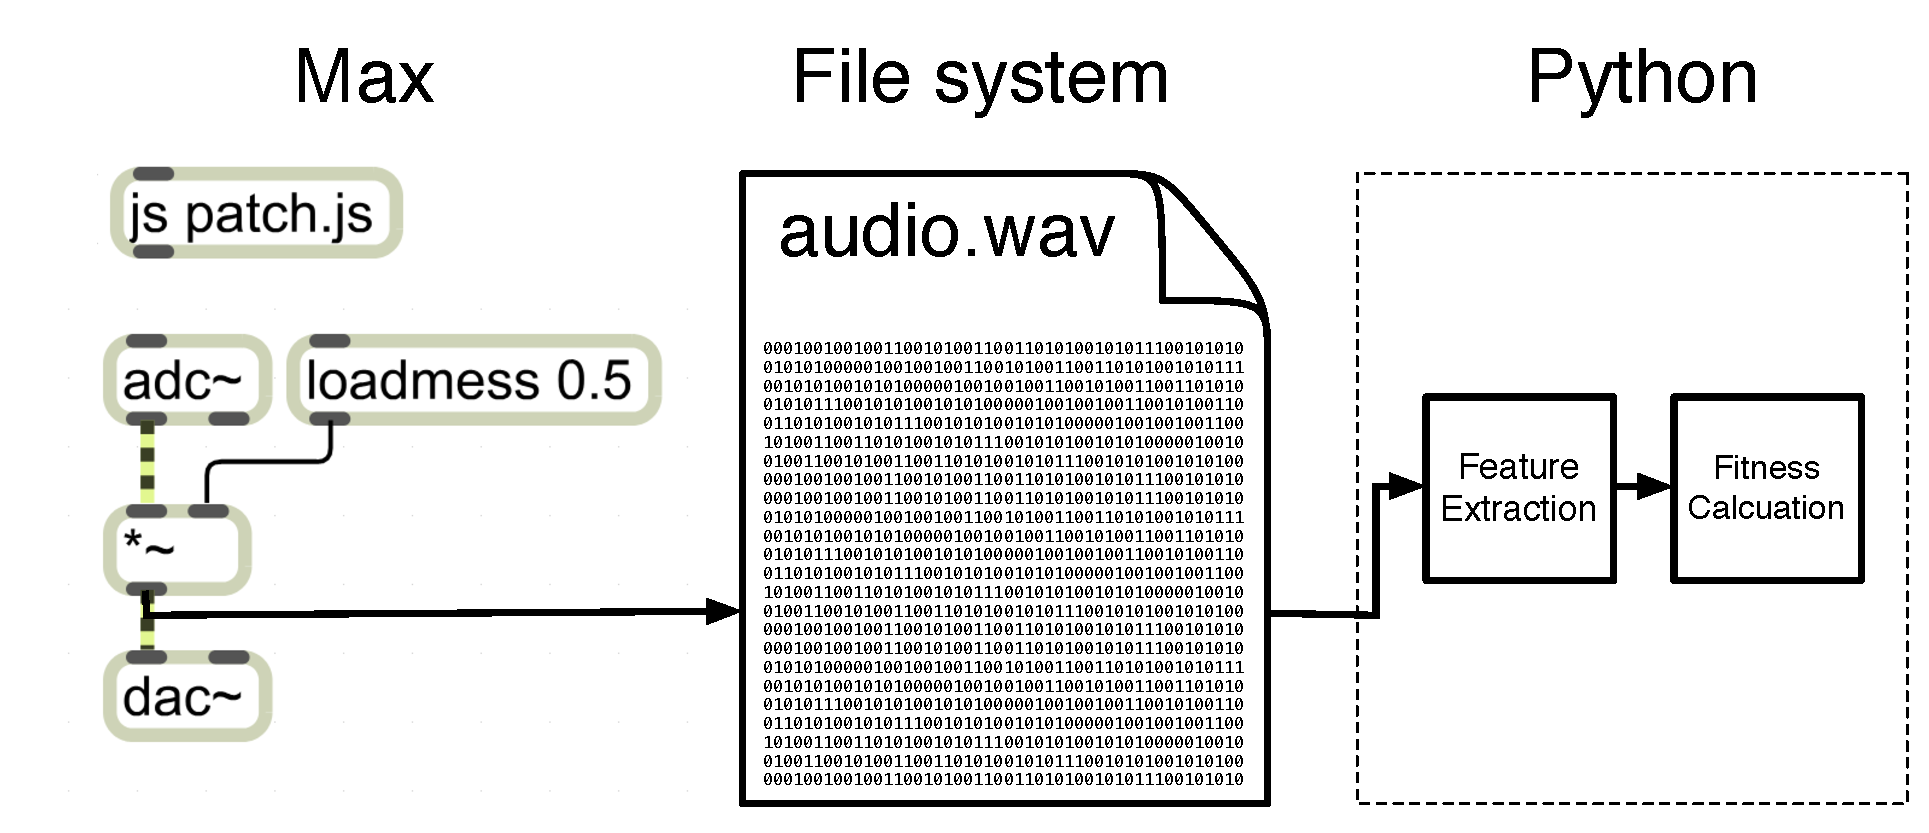
\includegraphics[scale=0.4]{MaxAudioToPython}
\caption{Writing audio output from a Max patch to a wav file that is then read and processed by Python code.}
\end{center}
\end{figure}
\\
In order for Python to have an internal representation of Max patches, we have mirrored all Max constructs using Python classes. For example, we have written MaxPatch, MaxObject, MaxInlet, and MaxConnection classes that represent patches, objects, inlets, and connections in Max. Therefore, the initial population creation is done in Python, the resultant patches are translated into JavaScript commands that, via Max's js object, are run in Max to generate the corresponding Max versions of the patches, an audio signal (more on this later) is sent through the patch, the output is recorded to a file, and Python reads in the file and uses its contents to calculate the fitness of the corresponding patch that produced it in order to apply genetic operators and create the next generation of patches.

\subsection{Framing as a Genetic Programming Problem}
The majority of GP research uses tree data structures to represent each individual algorithm within a population. We have adopted this representation in evolving Max patches that function as synthesis algorithms. Since Max, in general, allows the creation of graph structures, we have decided to limit the number of possible patch representations by enforcing several rules. 
\begin{enumerate}
\item The root of each tree will be Max's audio output object (the \emph{dac\texttildelow{}}), internal nodes will represent other Max objects are able to receive Max signal input and return Max signal output, and the leaf nodes or terminals will represent either audio generators (including audio playback objects and live audio input objects) or input parameters to the patch (see fig. 3).
\begin{figure}[h!]
\begin{center}
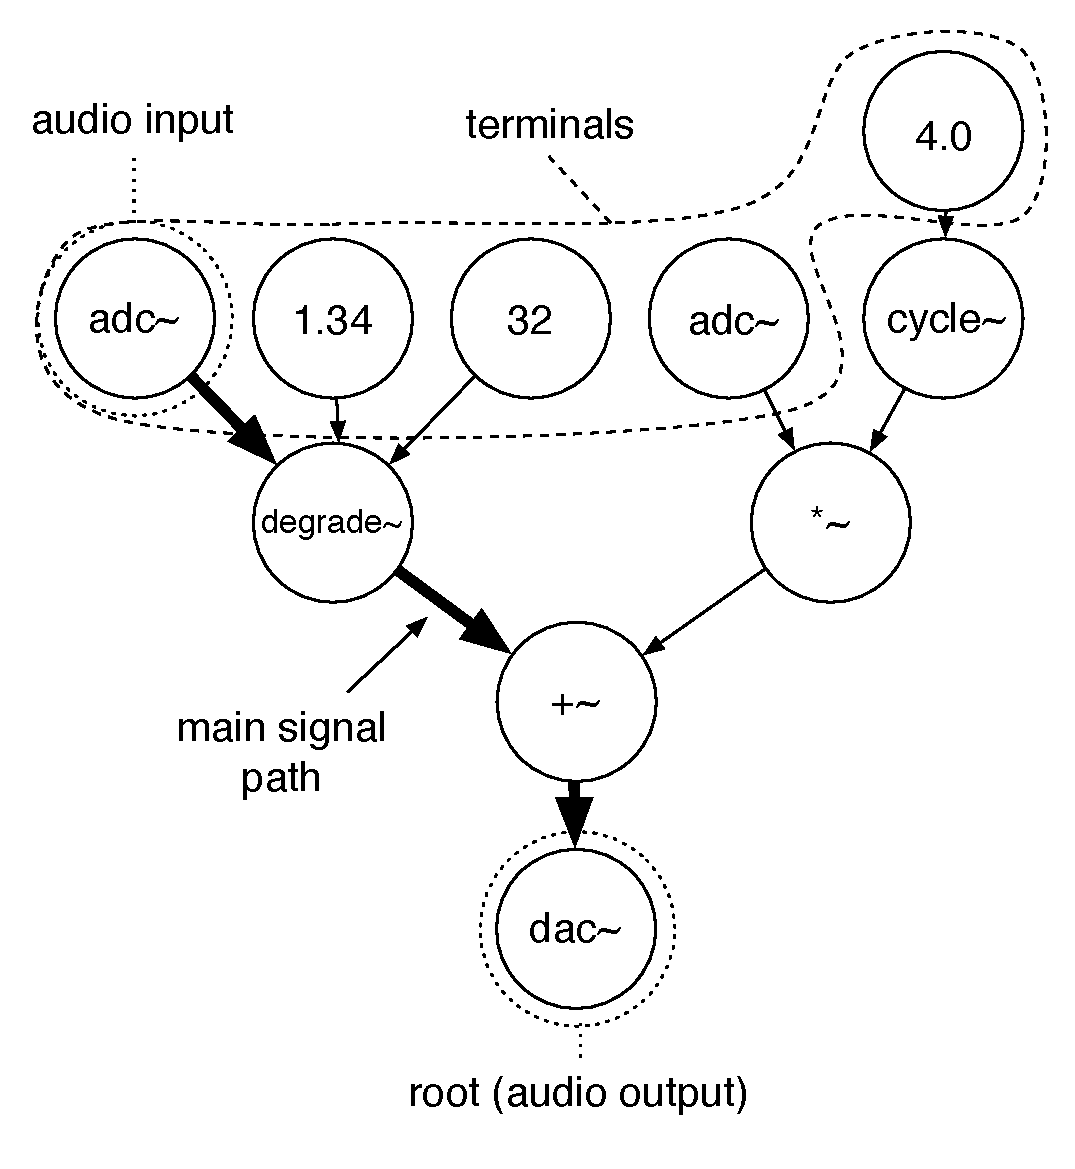
\includegraphics[scale=0.7]{RootTree}
\caption{An example Max patch represented as a directed tree with the audio signal flowing from patch's terminals towards its root.}
\end{center}
\end{figure}
\\
\item By ensuring that at least one terminal is an audio generator, a main signal path can be traced from the input object to the \emph{dac\texttildelow{}}, as seen in Figure 3.3. Therefore, the patch can be similarly viewed as a black box with audio going in and audio coming out---the fundamental representation of a synthesis algorithm. If more than one audio generator is chosen as a terminal, any could be viewed as that which produces the main signal path, while all others can be regarded as audio-rate input parameters to the system. Thus, the black box representation still holds.
\end{enumerate}

It should be noted that adhering to the above rules will restrict the search space over all Max patches. Any time such a search space restriction is put in place, one must make sure viable solutions are not left out of the resultant subspace over with the search will occur. Our goal is to search over the space of all synthesis algorithms and not over all Max patches (which occupies a much larger space), so as long as we can be sure that the above restrictions do not leave out any synthesis algorithms, we can proceed without worry.

Any Max patch can be easily be represented by a finite set of directed acyclic graphs (DAGs) - where directed edges correspond to Max connections with direction pointing from object outlet to object inlet and vertices correspond to Max objects (see Figure 3.4).
\begin{figure}[h!]
\begin{center}
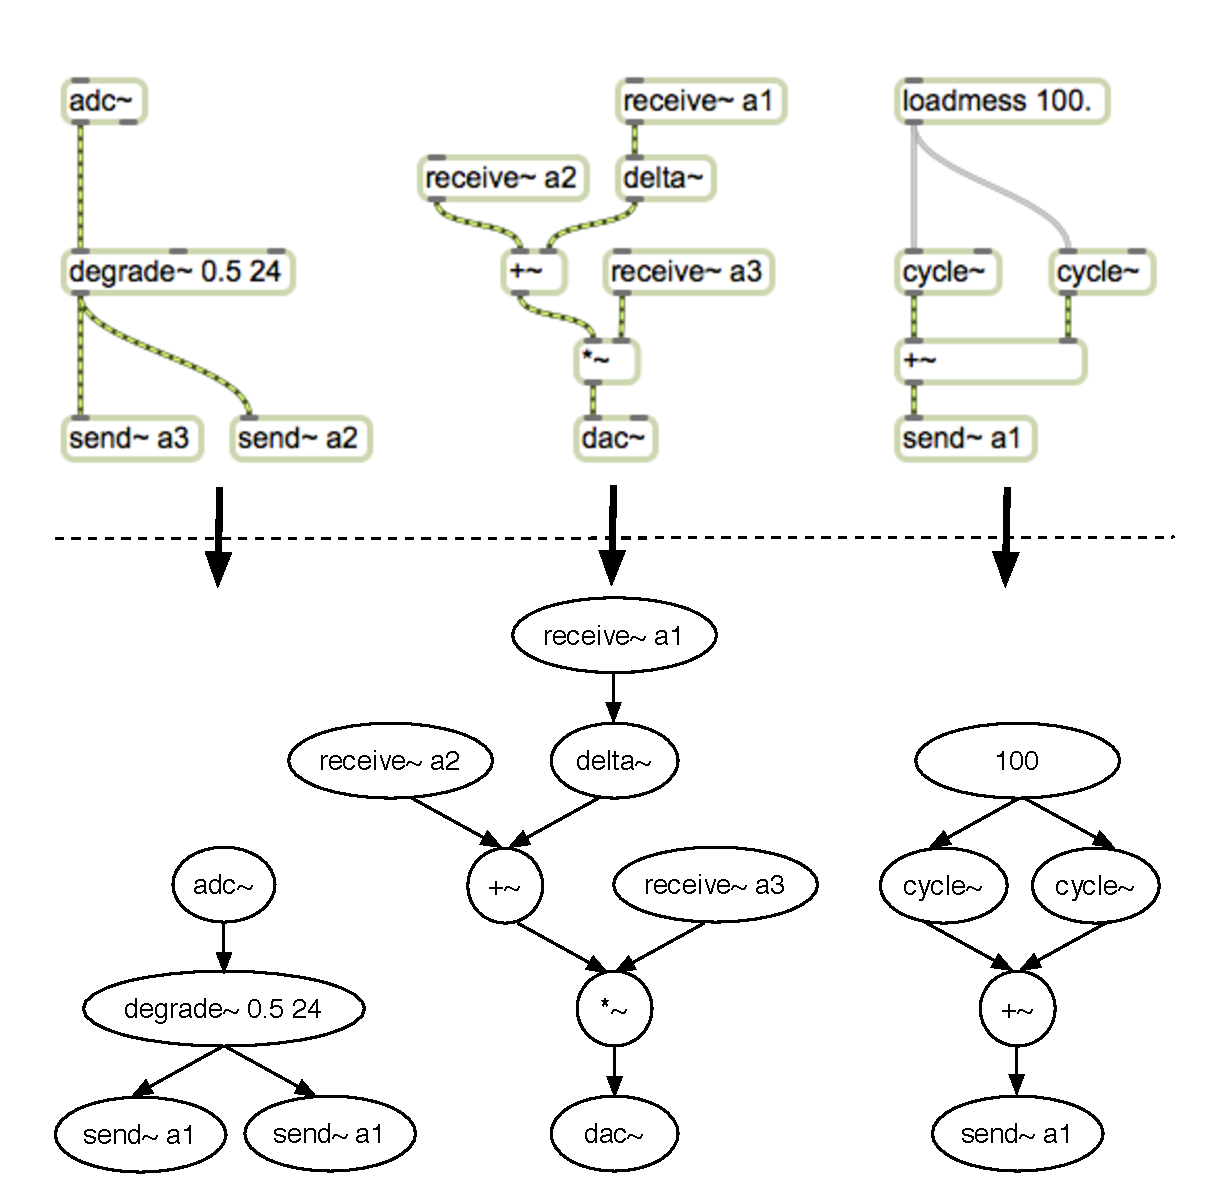
\includegraphics[scale=0.7]{MaxDAGs}
\caption{A Max patch and its corresponding representation as a set of DAGs}
\end{center}
\end{figure}
\\
In the case that a Max object would exist in a patch with arguments (as pictured in Figure 3.5) and no inputs attached to the inlets whose initial values are represented by those arguments, we can replace it with its default version (i.e. one without arguments) and with a set of connected \emph{loadmess} objects supplying those arguments and acting as terminals, thereby transforming a patch containing objects with arguments and exposed inlets to one with a more direct correlation to a set of DAGs.
\begin{figure}[h!]
\begin{center}
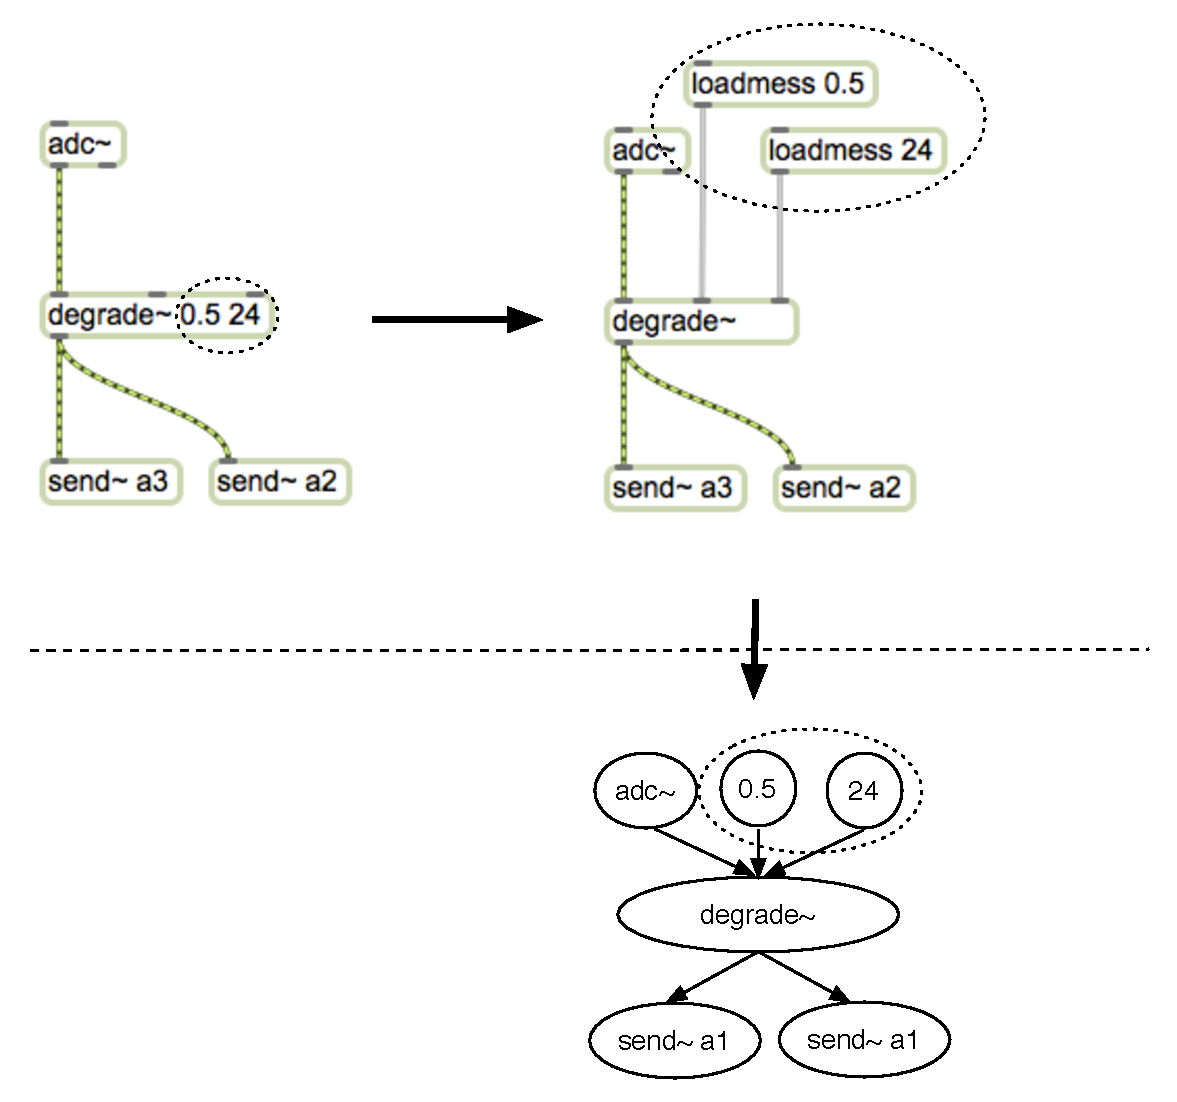
\includegraphics[scale=0.7]{MaxDAGsLoadmess}
\caption{The same \emph{degrade\texttildelow{}} object in two Max patches (one with arguments and one with load mess objects).}
\end{center}
\end{figure}
\\
Max objects come in a number of flavors with regard to what type of data can flow into and out from their connections. The objects that we are primarily interested in are Max's signal processing objects, which output Max's signal data type (i.e. data produced, transformed, and output at the patch's audio sample rate). While Max does provide mechanisms by which to convert from its other data types (e.g. matrices of video data, MIDI control rate data) to the signal data type, our research will focus only on the set of objects designed specifically to work with audio data. The terminating Max signal processing object for audio output via an audio device is the \emph{dac\texttildelow{}}. Since any signal processing algorithm must terminate at an output node of this type, the \emph{dac\texttildelow{}} will be required of any patch we wish to search over. If there is only one \emph{dac\texttildelow{}} in the patch, then only the objects in its directed acyclic graph will contribute to what is sent to the audio output device, unless there is another directed acyclic graph that terminates with a \emph{send} or \emph{send\texttildelow{}} object that passes data to a \emph{receive} or \emph{receive\texttildelow{}} object within the same DAG as the \emph{dac\texttildelow{}}. However, in this case, the send to receive connection could easily be represented by a directed edge and therefore we are still left with only one DAG with a \emph{dac\texttildelow{}} (see Figures 3.6 and 3.7).
\begin{figure}[h!]
\begin{center}
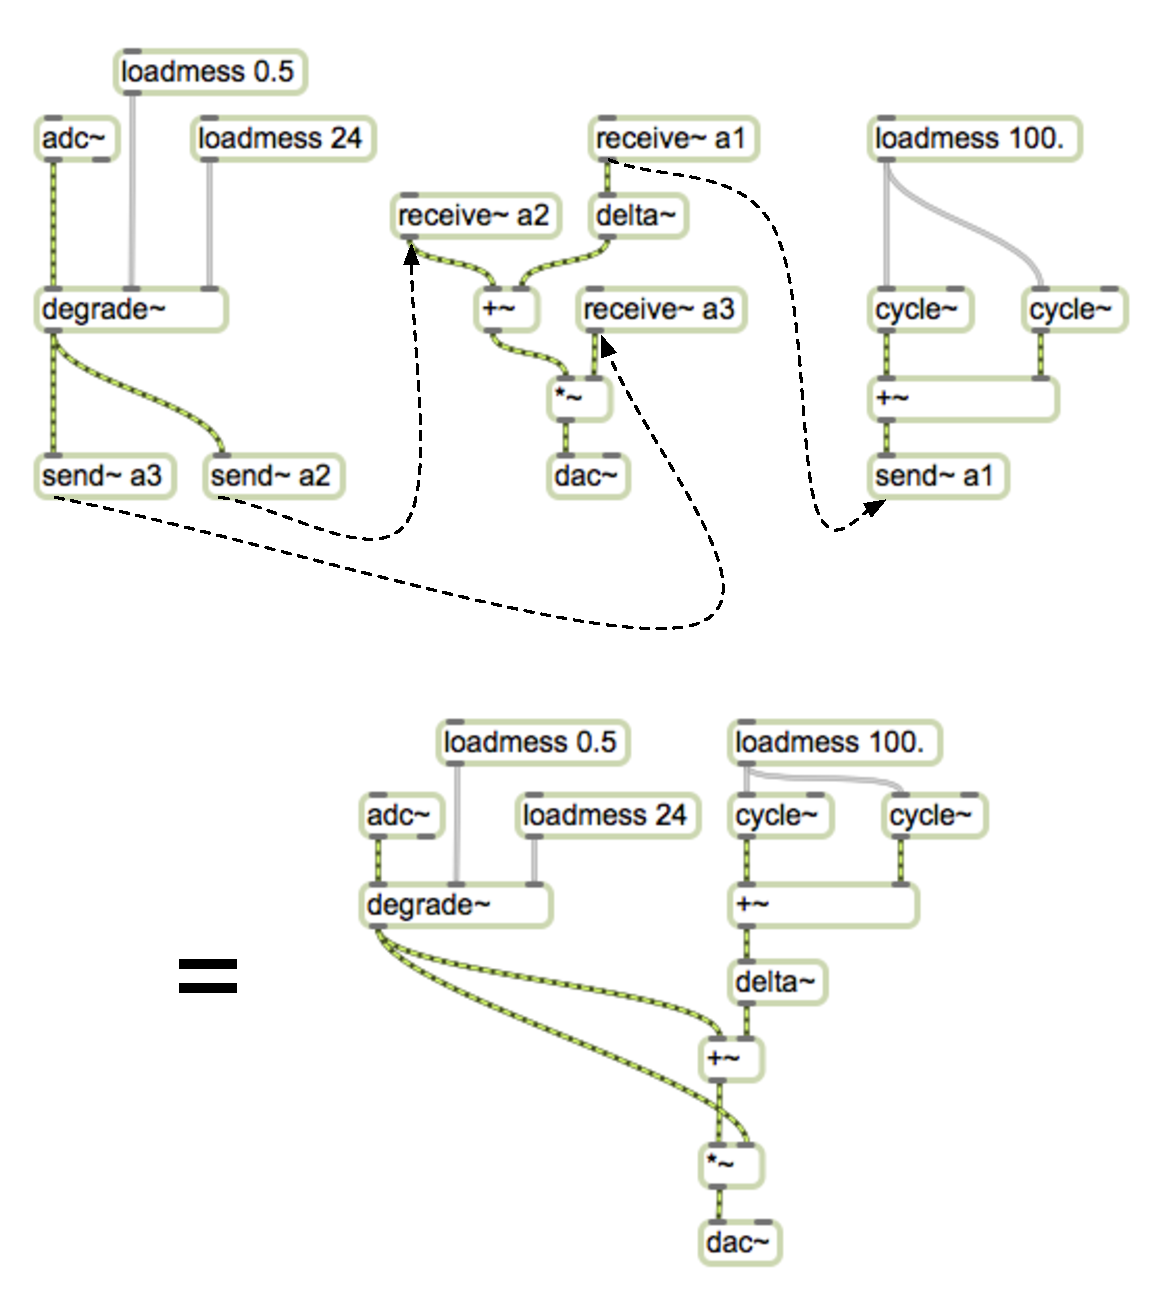
\includegraphics[scale=0.75]{MaxDAGsSendReceive1}
\caption{The original Max patch from Figure 3.4 replaced by its equivalent patch without send\texttildelow{} or receive\texttildelow{} objects.}
\end{center}
\end{figure}
\begin{figure}[h!]
\begin{center}
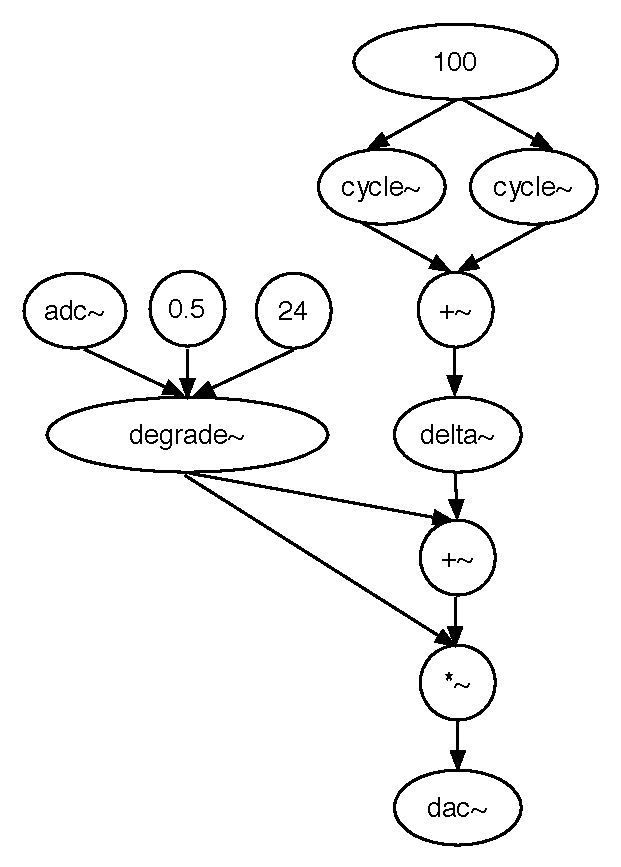
\includegraphics[scale=0.8]{MaxDAGsSendReceive2}
\caption{The single DAG representation of the reduced patch in Figure 3.6.}
\end{center}
\end{figure}
\\
If there are two or more \emph{dac\texttildelow{}} nodes in the DAG, the signals sent to them are simply summed before being sent to the audio output device. Therefore, we could easily model the same DAG with one \emph{dac\texttildelow{}} and one or more \emph{+\texttildelow{}} objects to sum all paths that would be summed by Max automatically (see Figure 3.8). 
\begin{figure}[h!]
\begin{center}
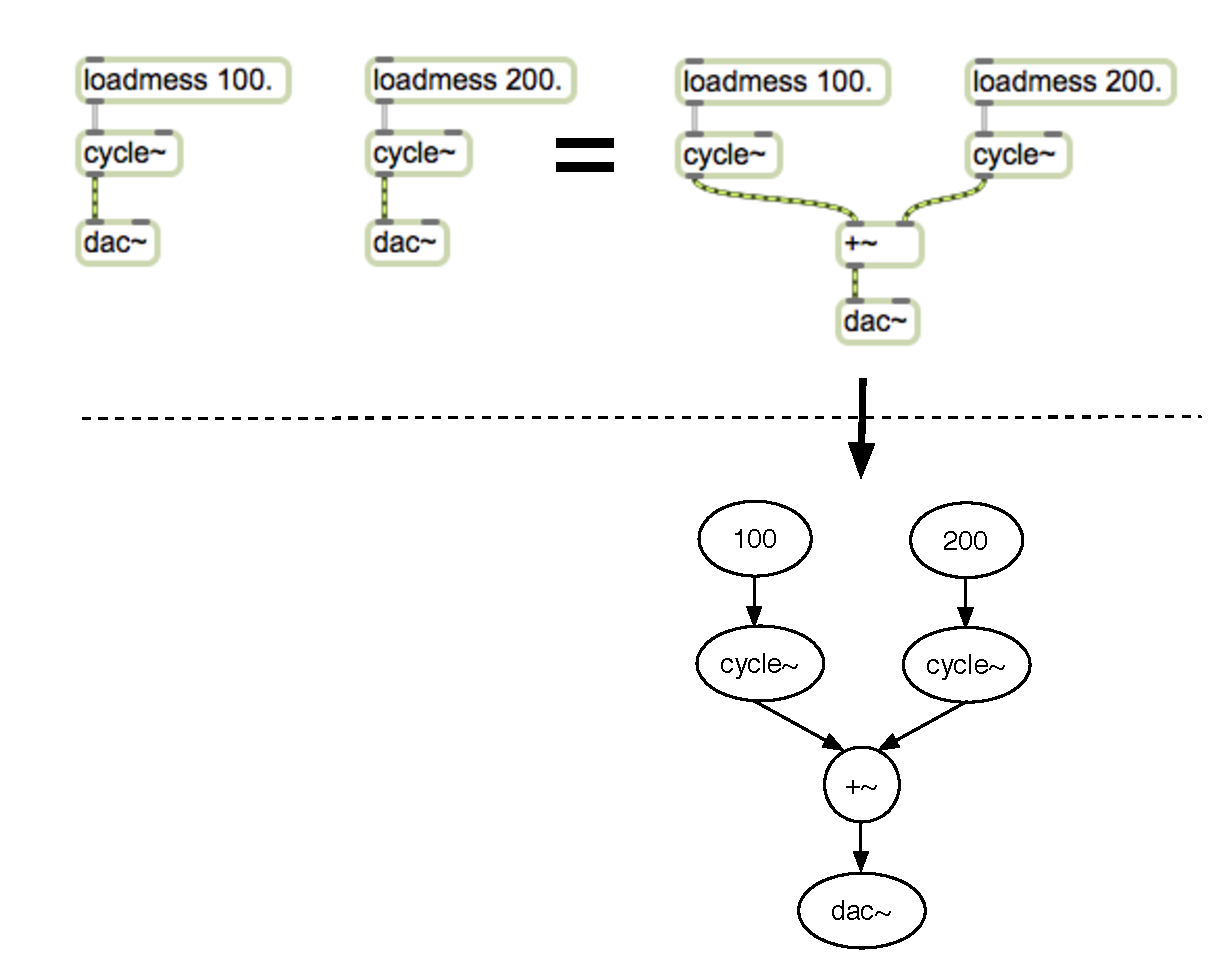
\includegraphics[scale=0.7]{MaxDAGs2DACs}
\caption{A single DAG representation of a Max patch with two \emph{dac\texttildelow{}} objects.}
\end{center}
\end{figure}
\\
Therefore, the only difference between the representation we've determined all signal processing Max patches can be reduced to and the tree data structure we are using to represent all patches within Python that we search over is that a tree data structure cannot have internal crossed paths. In other words, given two vertices u and v in our tree representation, there is at most one possible path connecting u and v. This is not the case for the DAG representation of all possible synthesis algorithms in Max that we have arrived at given the above arguments (see Figure 3.9 for an example).
\begin{figure}[h!]
\begin{center}
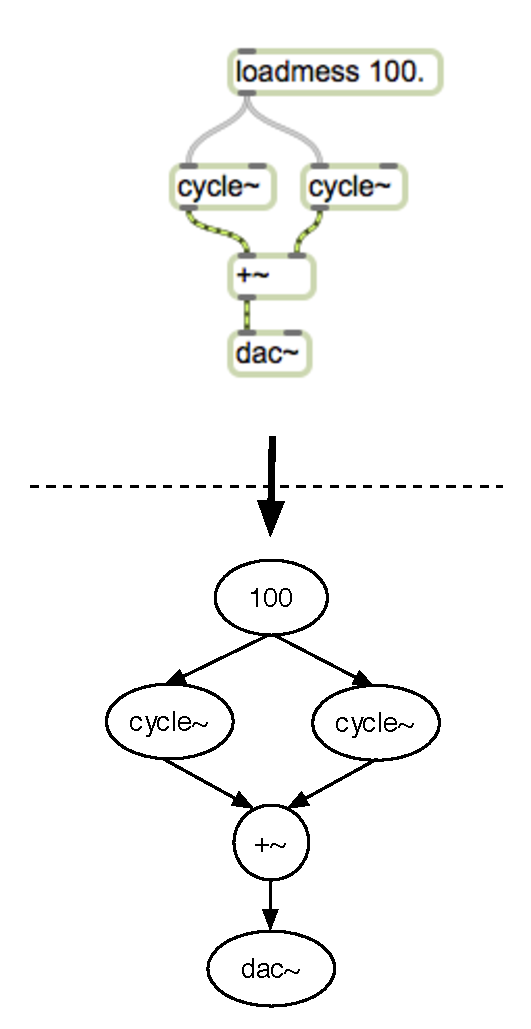
\includegraphics[scale=0.8]{MaxDAGsCrossedPaths}
\caption{A simple Max patch whose DAG representation has crossed paths and therefore is not a tree.}
\end{center}
\end{figure}
\\
However, for every possible DAG representation discussed, there is an equivalent tree representation that can be obtained by splitting each crossed path, duplicating all nodes below it (or 'above' it in the visual diagrams presented) for each node at the end of the crossed path (see Figure 3.10).
\begin{figure}[h!]
\begin{center}
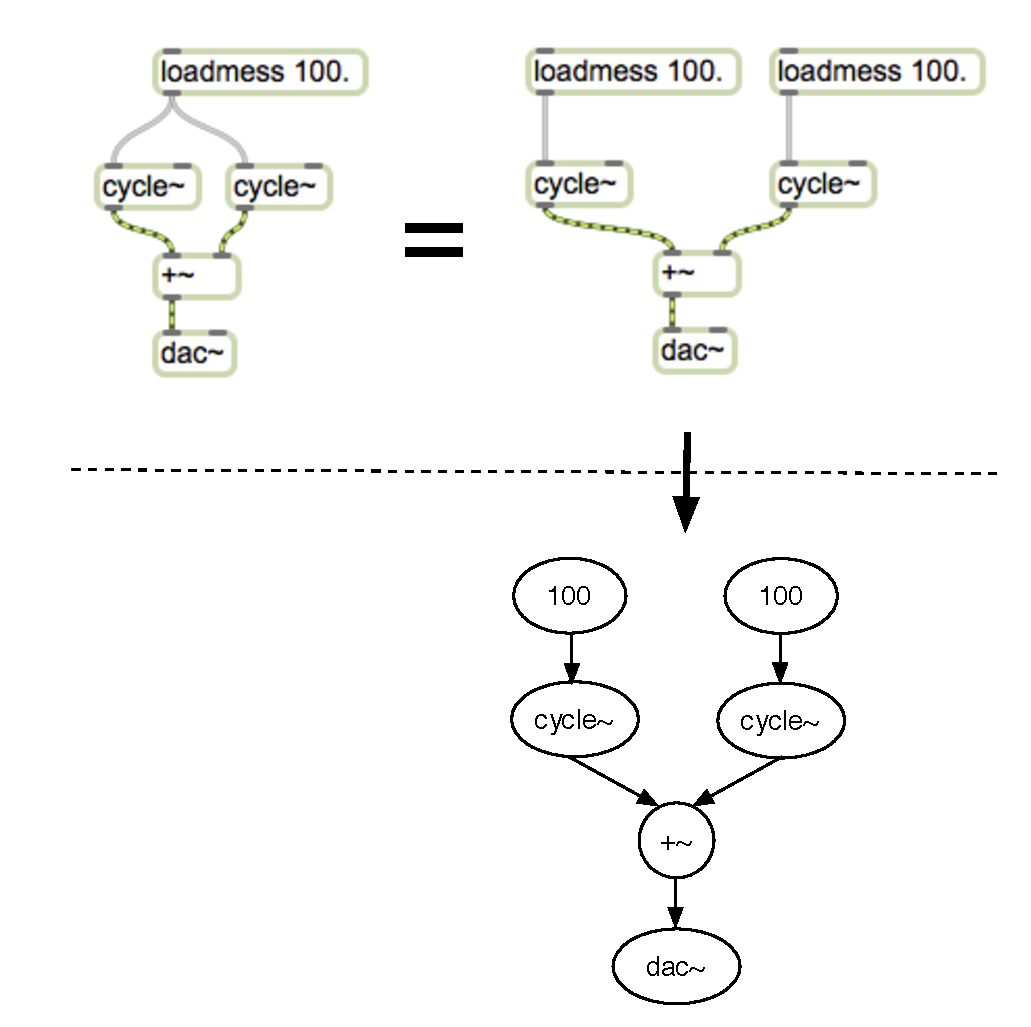
\includegraphics[scale=0.8]{MaxDAGsCrossedPaths2}
\caption{The same Max patch with crossed paths from Figure 3.9 and its equivalent Max patch with a tree representation.}
\end{center}
\end{figure}
\\
Taking all of the above arguments into account it is clear that by choosing the tree representation we have (which is necessary to leverage most work in the GP domain) we are not excluding Max synthesis topologies. 

It should also be noted that starting with a random tree representation of a Max patch can lead to patches that are not syntactically correct. Our trees are only valid representations of Max patches if their edges represent connections that are allowed in the Max environment. In other words, connections to inlets are valid only if the data flowing over those connections are accepted by the inlets. Therefore, syntactic correctness must be enforced while searching over the input-space defined by these trees. As previously noted in the discussion of strongly-typed GP, enforcing data type constraints during search is a simple way to disregard invalid topologies and make the search much more efficient without excluding possible solutions. We have therefore decided to incorporate knowledge of Max syntax into our system.

Information regarding syntactic correctness rules in Max is supplied to Python via a text file, which contains a list of Max object names, each followed by their respective inputs' accepted data types and reasonable input ranges, and their output data type (see Figure 3.11).
\begin{figure}[h!]
\begin{center}
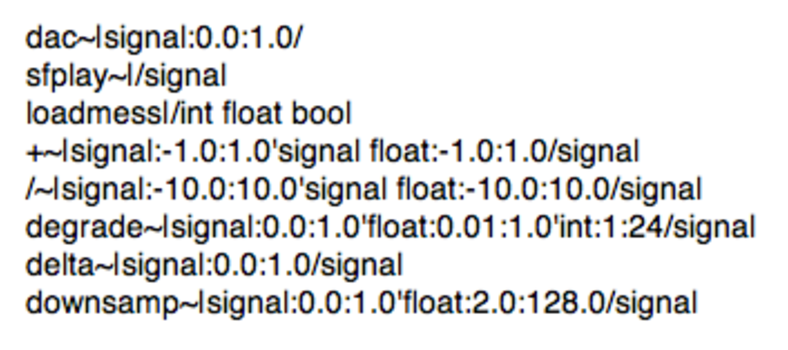
\includegraphics[scale=0.8]{SyntaxInfo}
\caption{Example of the object\_list.txt file that contains syntax information for the various objects used to generate patches with our system.}
\end{center}
\end{figure}
\\
The format is as follows where the inlet information is simply repeated for multiple inlets and the output type is repeated for multiple outlets (with spaces in between outlet types as shown in Figure 3.11):
\\
\textbf{\emph{objectName\textbar inlet1InputType:minVal:maxVal'.../outletType1 ...}}

`Reasonable ranges' must be chosen carefully as to not be too restrictive, since a particular object may be required to function outside of what is considered its norm in order to contribute to the best solution. Therefore, one of the variables we have decided to modify throughout our experiments are the sizes of the reasonable ranges for each object used. Even more importantly, it should be noted that the number of unique Max objects available for use in our system (and therefore the size of the patch space searched) is limited by how many objects we provide syntactic information for. Therefore, we have also investigated how our system performs by varying the number of objects in an attempt to determine whether a general set exists that is small enough for the search to provide a good solution over a reasonable amount of iterations, but also large enough to provide a solution that produces content that similar enough to the target to be considered a success. Specifics around the variation of both accepted inlet value ranges and object sets are provided in the Experiment Design section below.

By representing synthesis algorithms using the tree representation discussed above, the input space can be viewed as a set of such tree topologies, where each point in the space corresponds to a topology with a unique set of parameters and objects. This representation is the common representation for most GP systems and we can therefore leverage much of the research carried out in this field in order to produce an effective system.

\subsection{Genetic Programming System Overview}
The GP system that we have designed follows the typical GP blueprint at a high level. We will provide a brief overview of the mechanisms involved in such a system and then will discuss where we have chosen to experiment and in what ways. A more detailed treatment of Genetic Programming can be found in John Koza's book \emph{Genetic Programming: On the Programming of Computers by Means of Natural Selection} (Koza, 1992).

As mentioned in \textbf{Chapter 2 - Prior Work}, Genetic Programming is a parallel search technique; meaning that instead of starting by looking in one location in space and moving along some search path from there, Genetic Programming starts looking in many places at once and allocates more resources to those regions that show promise. The search process loosely models biological evolution and so borrows a number of terms from that domain. The number of points in algorithm space searched over at each iteration is defined as the current \emph{population}, with the first iteration starting with an initial population. The objective function that one wants to maximize over the search is referred to as the \emph{fitness function} and each successive iteration favors regions of space with higher fitness as it \emph{selects} individuals for the next \emph{generation} to \emph{mutate} and effectively `mate' in a process where algorithms swap pieces of their code in a process called \emph{crossover}. 

There are many variations of the operations (known as \emph{genetic operators}) used to \emph{evolve} algorithms from generation to generation and also the selection criteria for the algorithms that are subjected to these operations. The fitness function is problem-dependent and the quality of the solutions found using GP is completely dependent on how well it models the actual fitness of each algorithm with respect to the stated goal. Our efforts in evolving Max patches have led us to explore all facets of GP in depth and we have found, as will be detailed in \textbf{Chapter 4 - Results}, that varying some meta-parameters have a large impact on solution quality, while others seem to have very little. Figure 3.12 shows a high-level flow diagram of our GP system with components marked off by what sub-sections in \textbf{3.2 Experiment Design} they are discussed.
\begin{figure}[h!]
\begin{center}
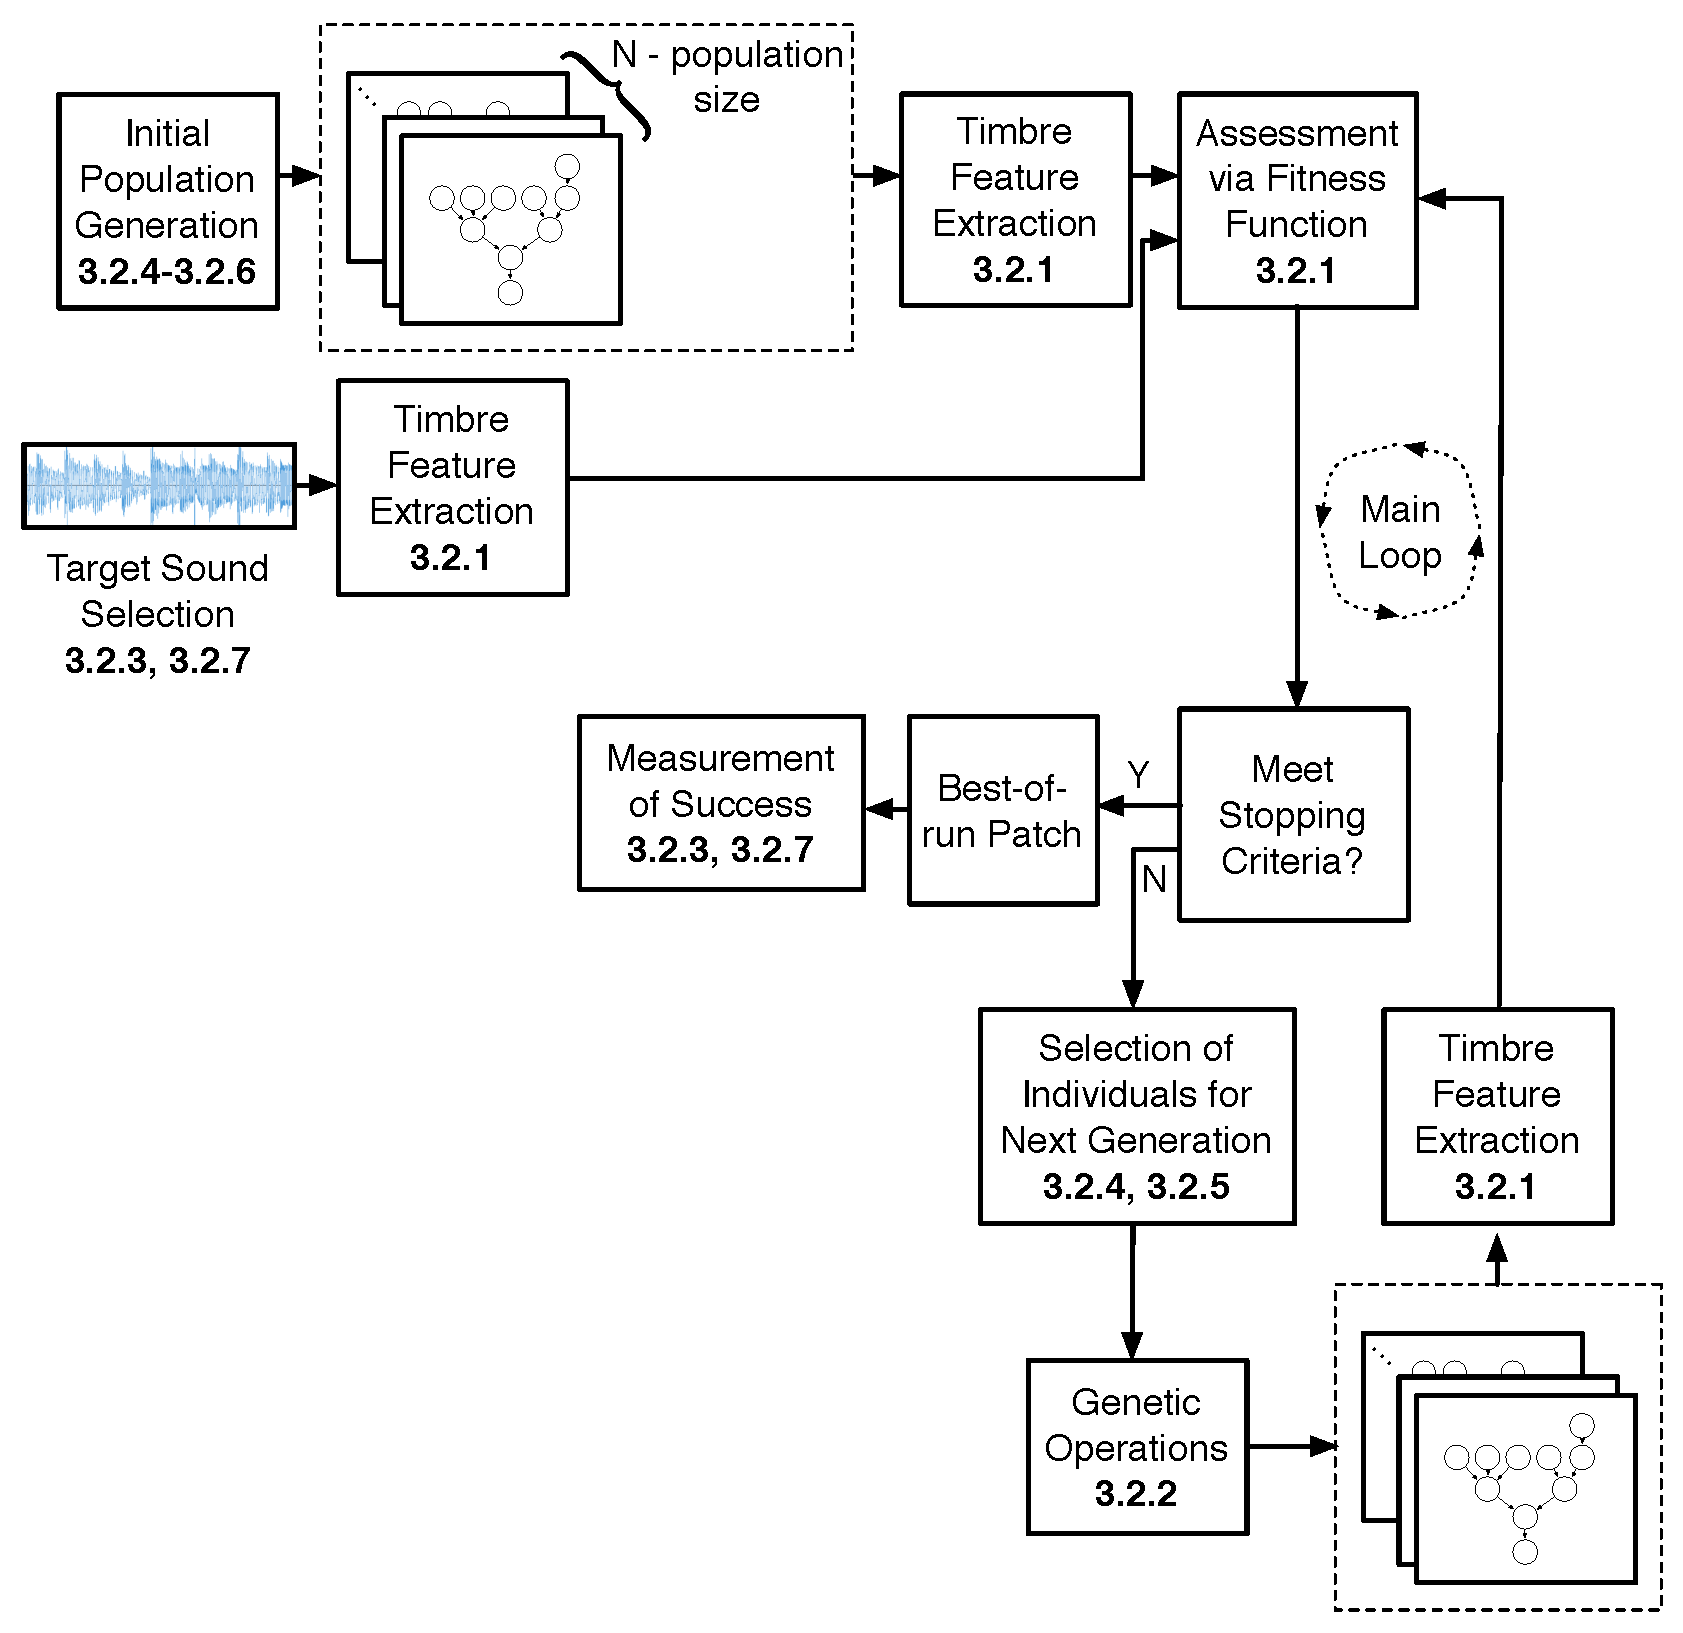
\includegraphics[scale=0.5]{OverallGPSystem}
\caption{Flow diagram of our GP system with components labeled by the section numbers they are discussed in.}
\end{center}
\end{figure}
\\
\clearpage
\section{Experiment Design}
As can be seen in Figure 3.12, there are several modules that make up our sound synthesis search system. Each module represents at least one variable of the system that contributes to its ability to find the optimal solution as quickly (i.e. within the smallest number of iterations) as possible. Given the high-dimensionality of this variable set, it is infeasible to perform an appropriate search over all of its various permutations within a reasonable amount of time. We have chosen instead to take a measured approach to varying each variable - while holding all others constant and comparing its various values/methods using key metrics designed specifically for it - by first looking at those variables that we believe have the least amount of dependence on the settings of all others and stepping through towards those that are most dependent. Using this approach, we will be able to treat the highly dependent variables given a fixed set of near-optimal values/methods for all other variables, thereby decreasing the chance that any noticeable shortcomings of a chosen value/method for one variable are actually a result of the sub-optimal configuration of other variables that directly influence the measure we use to test it.

With this methodology in mind, we have chosen to first examine our fitness function, as it will be required to measure the success of various flavors of our system.

\subsection{The Fitness Function}
Defining the fitness function is how one communicates to the GP system what their objective is. Without an appropriate definition, the system may discard more-optimal solutions for less-optimal ones in the eyes of the developer. This is not a shortcoming of the system itself, but instead of the developer's ability to accurately convey to the system what he is looking for. It is therefore paramount to a system's ability to produce optimal solutions to provide it with a fitness function that objectively measures the usefulness of any given solution in the same way the developer would assign value.

In this research, our objective is to generate Max patches that are able to successfully produce audio that is timbrally similar to some target sound. In order to define a fitness measure for this objective, we need to have a definition of timbre similarity. Before we can discuss an objective timbre similarity measure, we first need to have a quantitative measure of timbre. Therefore, the first task we face is choosing an appropriate timbre feature.

\subsubsection{Timbre Feature Extraction}

The design of a semantically valid objective timbre space is paramount to the problem of search. If a timbre space has not be chosen such that meaningful timbre similarity measurements can be made, then the fitness landscape will be ill-formed and the search will pursue areas of the input space that are not relevant to the problem.

As previously discussed in the Prior Work, obtaining a ground truth to evaluate against is problematic. While most timbre space evaluation is indirectly performed via (instrument) classification tasks, due to the cost of doing large scale subjective testing, this evaluation typically assumes that all sounds produced by the same instrument have the same or similar timbre, regardless of playing technique, and so it is not clear whether or not similar evaluation methods will be valid for the �type� of timbre we are interested in. In a recent paper by Pampak, Herrera, and Goto, in referring to timbral studies that use instrument classification as a means of evaluation, the authors note that �instrument class data only allows comparison on the instrument level. Judgements within an instrument class cannot be evaluated directly� (2008, p. 9).

However, if we assume that, in general, sounds from the same instrument should cluster well in a semantically meaningful timbre space (i.e. the ratio of variance between classes/instruments should be much greater than the variance within classes/instruments), we can infer that any timbre space with that property will be organized at a high-level similarly to the optimal space. The low-level organization of the optimal space (within instrument group organization) may differ with some members of the subset of timbre spaces that have similar high-level organization and so a more rigorous treatment should be carried out to verify the appropriateness of a timbre space that organizes instrument classes well, but we leave this treatment to future work. Therefore, we assume it is enough to show that the timbre measure that we will use performs at the level of the state-of-the-art instrument recognition systems when paired with a simple classifier, like Nearest Neighbor (NN).

This relationship between classification performance and timbre space suitability provides an indirect means of testing a given timbre space. By using an unsophisticated classifier, we fully expose the organization of the space and how well instruments are clustered within it; things that could be masked by a sophisticated classifier able to overcome minor faults in both.

Nearest Neighbor classification in our case consists of mapping a large database of instrument sound samples into the objective timbre space and measuring how well they cluster by instrument by randomly choosing samples in the space, searching for their nearest neighbor in that space, and recording whether that neighbor was produced by the same instrument. One is then able to compare multiple objective spaces by using the �classification� accuracy found during the experiment. This method is often extended to reduce noise by selecting k-nearest neighbors (kNN) and noting how many of the k neighbors were produced by the same instrument as the test sample (see Figure 3.14).
\begin{figure}[h!]
\begin{center}
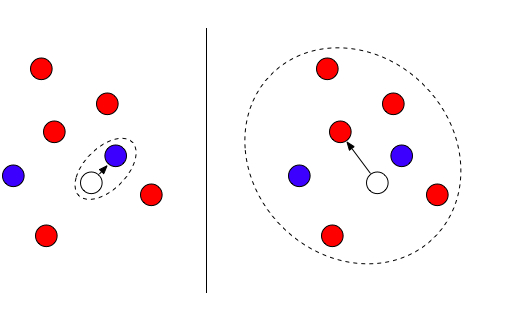
\includegraphics[scale=0.5]{NearestNeighbor}
\caption[Nearest-neighbor vs. k-nearest neighbor classifier]{Nearest-neighbor vs. k-nearest neighbor classifier - the test sample (white) is set to the blue class in nearest-neighbor classification and to the red in k-nearest neighbor classification where k = 7}
\end{center}
\end{figure}
\\
Given the above, we have decided to measure the appropriateness of a given objective timbre space by running an instrument classification experiment on it using a kNN classifier.

In a paper we have helped author \cite{Humphrey:2000th} we discuss our belief that it is `advantageous to automatically learn features from some minimally processed input representation' rather than hand-craft a feature set that would produce a semantically meaningful timbre space. In short, learning features allows one to explicitly specify how they want a feature-space organized (in our case, well-clustered instrument samples) and leverage machine learning algorithms to find an optimal space for that criteria, whereas designing features based either on perceptual models or what one believes to be the important information content related to a task is just a guessing game with no proven iterative search strategy, likely excluding optimal solutions simply because they are non-intuitive or obfuscated from the researcher in some way.

The technique that we have helped develop to learn an appropriate timbre space where different instruments are well-clustered is titled `Non-linear Semantic Embedding (NLSE).' In our paper we note:
\begin{quote}
NLSE addresses the limitations of current statistical dimensionality reduction techniques, such as MDS, PCA or LLE [because] unlike these methods, NLSE explicitly encodes semantic information in the transformation, makes minimal assumptions about salient acoustic features, generalizes well to unseen data and produces an output space where [Euclidean] distance is meaningful.
\end{quote}

NLSE utilizes a pairwise Convolutional Neural Net (CNN) model based upon Hadsell, Chopra, and LeCun's work on Dimensionality Reduction by Learning an Invariant Mapping (DrLIM) (2006). CNNs are a special kind of Neural Net that combines convolutional layers (where inputs are convolved with 2D filters, whose values are trainable) that are typically separated by a downsampling operation and a non-linear squashing function (see Figure 3.14). After a succession of these convolution layers, CNNs most often use standard fully-connected NN layers to reduce the dimensionality of the data before output. The benefits of CNNs are found in the translation invariance their convolutional layers provide, and scale invariance the downsampling operation provides. When the input to a CNN is a time-frequency representation as is the case in our problem domain, these invariances correspond to small invariances in temporal shifts and scalings in our data (important because we should not suppose that all samples will be precisely temporally aligned or that their timbral information will evolve precisely in the same manner) and small invariances over our frequency scale. The latter invariance is important to extracting timbre from a signal, because it is generally believed that timbre does not correlate with pitch variation. It is therefore possible to utilize the inherent frequency scale invariance that CNNs provide to better eliminate any dependencies in our output space on pitch by using a time-frequency representation that is linear in pitch. For this reason, we have chosen a constant-Q time frequency representation as is shown in Figure 3.14, where bins are spaced equally in pitch space rather than in frequency space.

Hadsell, Chopra, and LeCun's work on DrLIM utilizes a pairwise CNN architecture (ie. two CNNs with the same exact structure) with tied weights to learn a low-dimensional invariant mapping from a high-dimensional input space. The training phase consists of sending both positive (i.e. samples from the same instrument) and negative (samples from two different instruments) examples through the CNNs and adjusting the tied weights such that semantically similar items are placed near each other in the output space and semantically dissimilar items are placed far away from each other in the output space. This is accomplished using what is known as a `contrastive loss function.' The basic idea is that one establishes a loss function that returns small values for positive examples that are close to one another in the output space and large values for positive examples that are far away from one another in the output space and conversely returns small values for negative examples that are far away from each other in the output space and large values for negative examples that are close to each other in the output space. Specifically, the loss function we have chosen that meets this criteria follows:
\begin{equation}
L(X_1, X_2, Y|W)=Y*L_{sim}(D)+(1-Y)*L_{Diff}
\end{equation}
The inputs $X_1$ and $X_2$ to L represent our constant-Q time-frequency patches, Y is our semantic similarity score between our inputs taking a value $[0,1]$ and W represents the parameters of the CNN architecture. $L_{Sim}(D)$ and $L_{Diff}(D)$ are our similarity loss and difference loss, respectively and D is some cost function associated with the outputs of our architecture, often labeled $Z_1$ and $Z_2$. In our system, this cost function is simply the Euclidean distance between the points $Z_1$ and $Z_2$.

Note that the only contributor to our contrastive loss, L, is the similarity loss when $Y=1$ (i.e. the items are maximally similar) and the only contributor to L is the difference loss when $Y=0$ (i.e. the items are maximally dissimilar). Since we want the loss to increase for similar items that are far apart, we chose the following similarity loss (known as the square loss):
\begin{equation}
L_{Sim}=\frac{1}{2}Y*D^2
\end{equation}
Note that as the distance between points increases, so does the loss. Conversely, we want the difference loss (which contributes most when items are maximally dissimilar) to increase as the distance between $Z_1$ and $Z_2$ decreases. We therefore chose the following difference loss (known as the `log-loss'):
\begin{equation}
L_{Diff}=\frac{1}{2*Q^2}*log\Big(1.0+e^{Q*(m-D)}\Big)^2
\end{equation}
The parameters $m$ and $Q$ are used to define the loss function's `margin' and `knee' respectively, but the details of this are not important. The important thing to note is that as $D$ decreases, $e^{Q*(m-D)}$ increases, which in turn increases $L_{Diff}$ as desired.

By using standard back propagation methods, one is able to update all the trainable parameters in the CNN architecture so that, over $N$ iterations, the parameters converge to a stable state (and hopefully a global optimum). Once convergence occurs, the resulting pairwise architecture represents two copies of a CNN that has learned a low-dimensional invariant mapping from the high-dimensional input space of your original data (e.g. patches of constant-Q spectra) into a semantically meaningful low-dimensional space. In our problem domain, this means a timbre space where samples from the same instrument class are well clustered and instrument clusters are well-separated.
\begin{figure}[h!]
\begin{center}
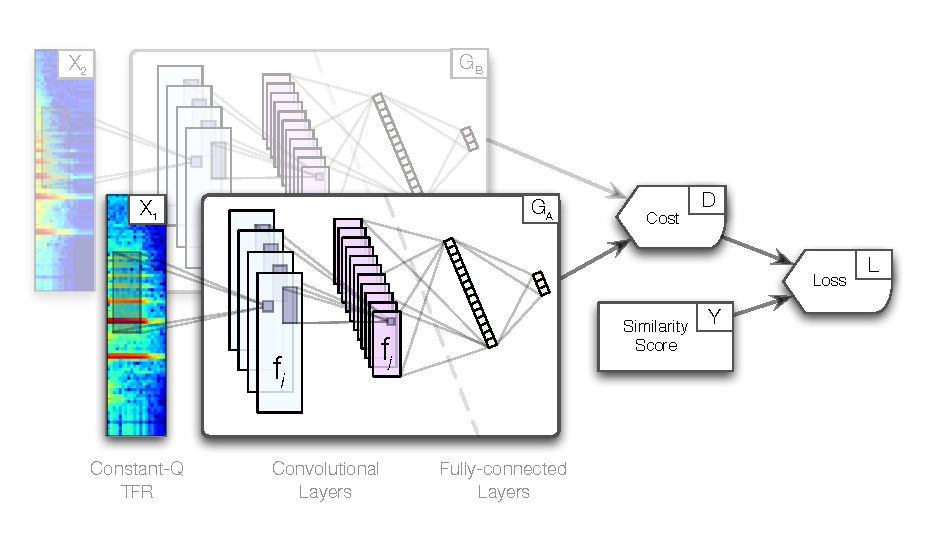
\includegraphics[scale=0.95]{PairwiseCNN}
\caption[Pairwise CNN Architecture]{Pairwise CNN used to learn an objective timbre space from various pairs of within class and between class instrument samples.}
\end{center}
\end{figure}
\\
As is shown in our paper, the objective timbre space we have generated (and the corresponding features that define the space) outperform the leading alternative timbre-feature in the literature (MFCCs) - after the typical PCA and LLE dimensionality reduction techniques have been applied - on instrument classification tasks involving up to 12 different instruments (see Figure 3.15 for kNN accuracy up to 9 instruments). Specifically, NLSE remains at a classification accuracy above 90\% until 7 instruments are introduced, while PCA and LLE are both between 30\%-40\% lower than NLSE for all cases.
\begin{figure}[h!]
\begin{center}
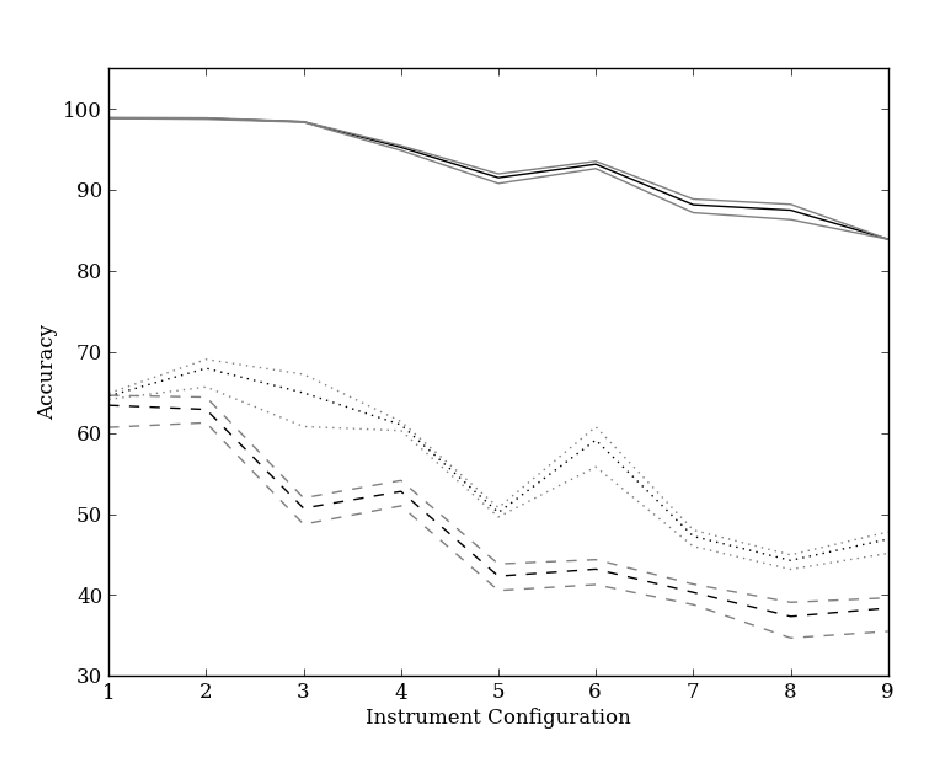
\includegraphics[scale=0.85]{CNN_kNN}
\caption[kNN accuracy for NLSE, PCA, and LLE]{The mean, min, and max kNN accuracy for experiments varying k using NLSE (solid lines), PCA (dotted lines), and LLE (dashed lines).}
\end{center}
\end{figure}
\\
For some intuition on how the objective timbre output spaces are organized in the NLSE, PCA of MFCC, and LLE of MFCC cases, see Figure 3.16 showing the distribution of instrument samples for 5 different instruments.
\begin{figure}[h!]
\begin{center}
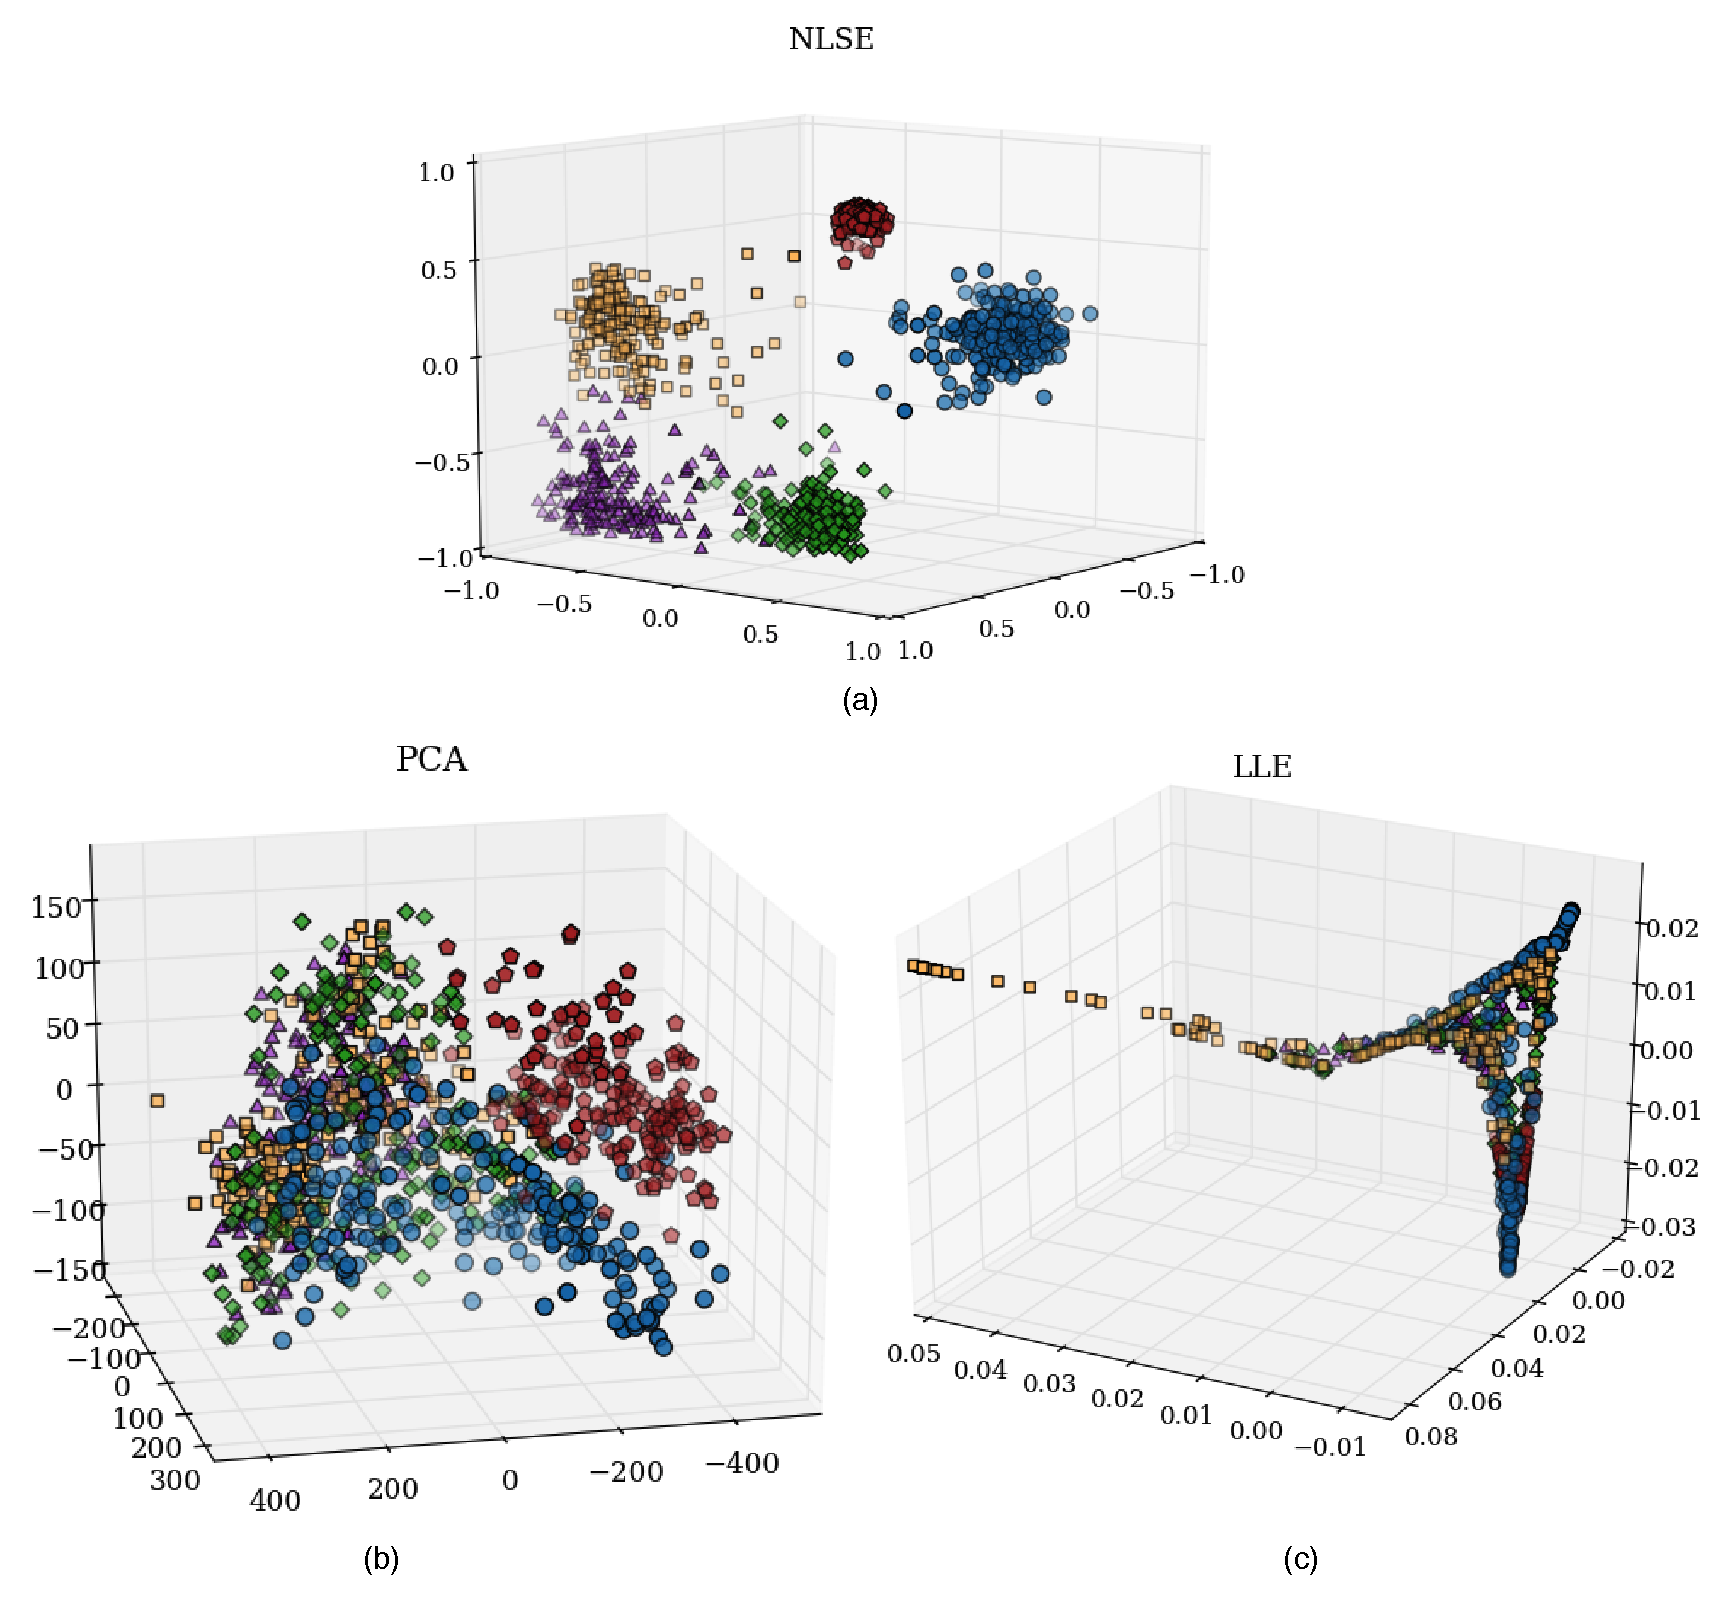
\includegraphics[scale=0.55]{NLSECluster}
\caption[NLSE vs. PCA vs. LLE Instrument Clusters]{Output feature spaces generated by (a) NLSE, (b) PCA, and (c) LLE for Tuba (red pentagons), Oboe (green diamonds), Clarinet (purple triangles), Cello (blue circles), and Flute (yellow squares).}
\end{center}
\end{figure}
\\
\subsubsection{Timbre Similarity}

Given the timbre features we have developed using CNNs, we must develop a measure of timbre similarity for time-varying timbres in the space our features define. Timbres that do not vary over $N$ time-frequency patches will only occupy a small region or point in this space. The calculation of timbre similarity between static or near-static timbres of this sort can simply be approximated using the Euclidean distance between the individual distribution centers since the space is trained for this distance to be semantically meaningful (see Figure 3.17). 
\begin{figure}[h!]
\begin{center}
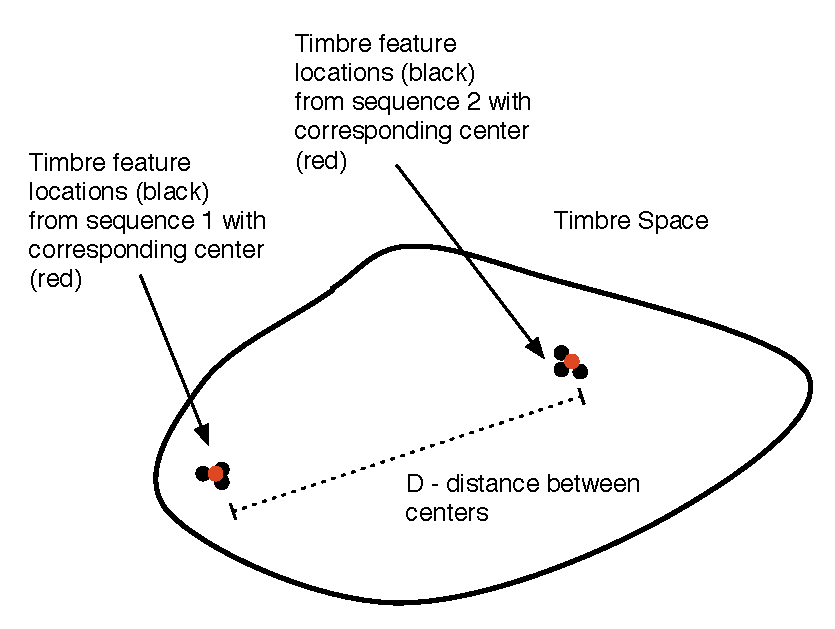
\includegraphics[scale=0.8]{TimbreDistance1}
\caption[Timbre Distance Between Centers]{Timbre similarity between two sequences of time-frequency patches approximated using the distance between their centers.}
\end{center}
\end{figure}
\\
However, the calculation of timbre similarity becomes more complicated once a sound contains timbal variation corresponding to a traced out path in timbre space away from the region in which it started. The task then becomes measuring similarity between two traced out paths in timbre space (see Figure 3.18). 
\begin{figure}[h!]
\begin{center}
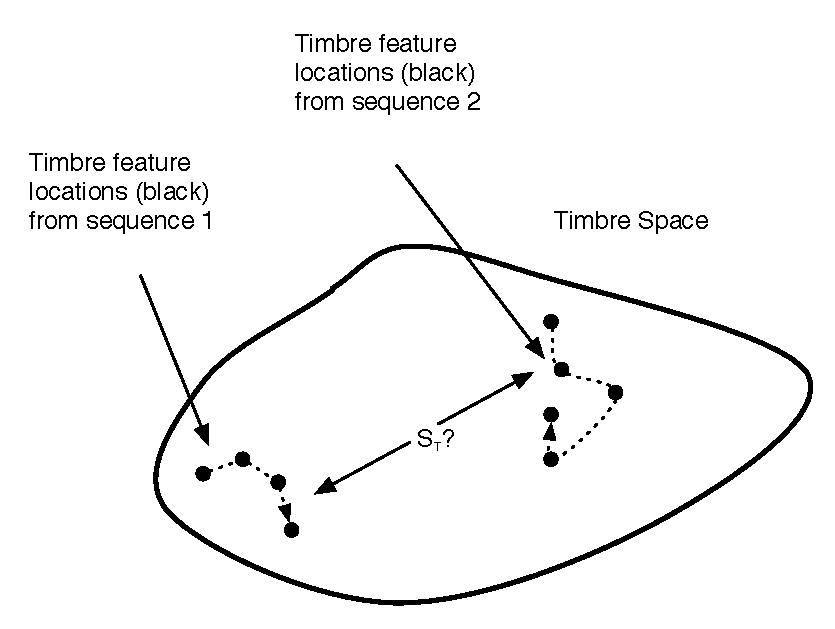
\includegraphics[scale=0.8]{TimbreDistance2}
\caption[Timbre Distance Between Curves]{How does one calculate the similarity or distance between two curves in timbre space that are not well localized?}
\end{center}
\end{figure}
\\
Since points in timbre space will occur at regular discrete intervals in time, the paths actually represent discrete sequences of timbre points. Therefore, the question we must answer is "How should one measure the timbre similarity between two discrete sequences (possibly having different lengths) of timbre feature vectors?" If we only allowed comparisons between sequences of equal length, a common solution would be to line up points in the two feature vector sequences, calculate the Euclidean distance between the pairs of lined up points, sum all distances, and take the inverse of the result (referred to as the `aligned-Euclidean' method going forward):
\begin{equation}
S_T = \sum_{i=1}^{M}\sqrt{\sum_{j=1}^{N}(Z_{ij}^1 - Z_{ij}^2)^2}
\end{equation}
where $Z^1$ and $Z^2$ represent the two sequences of timbre feature vectors (obtained via processing of time-frequency patches through our trained CNN architecture) to compare, N is the dimensionality of the timbre feature space, and M is the length of each sequence.

However, even given the restriction of equal sequence lengths (which is obviously undesirable) there are many examples where this measure will break down. For example, if one takes two copies of the same exact sound and applies a simple linear time shift to one (i.e. a delay), the suggested similarity calculation could result in labeling the two sounds as being very distant (see Figure 3.19).
\begin{figure}[h!]
\begin{center}
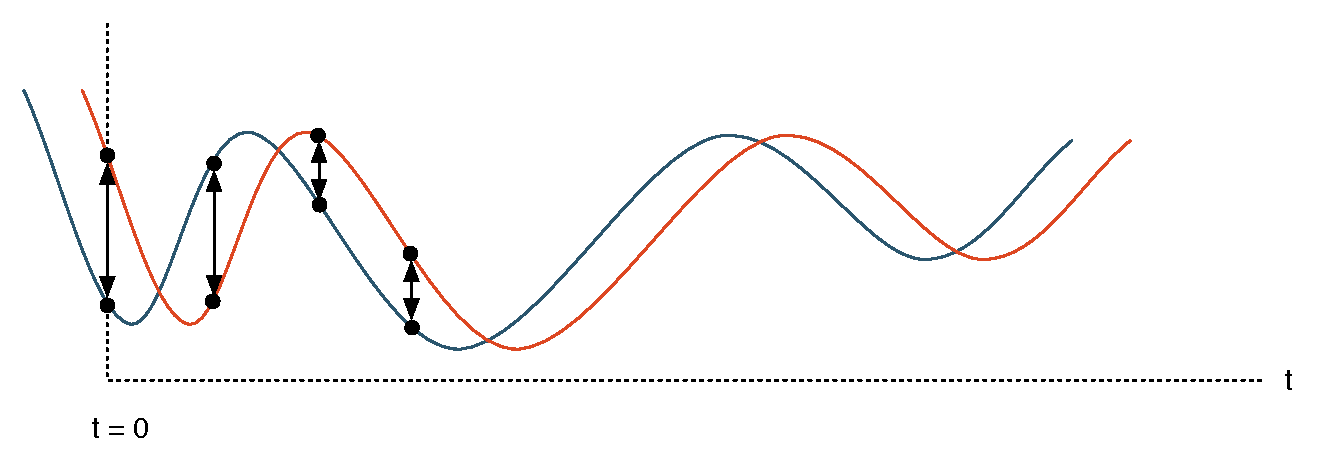
\includegraphics[scale=0.6]{TimbreDistance3}
\caption[Timbre Distance Between Time-Shifted Curves]{An example of how a simple temporal shift of the exact same curve can result in non-negligible distance calculations between corresponding points in the resultant discrete sequences.}
\end{center}
\end{figure}
\\
Slight time warpings of one sound compared to the other would also result in an incorrect assessment (see Figure 3.20). It is for this reason that Jehan uses Dynamic Time Warping (DTW) when calculating similarity over sound segments (2005). The only difference between the problem he was addressing and ours is the time scale on which similarity is being computed. 
\begin{figure}[h!]
\begin{center}
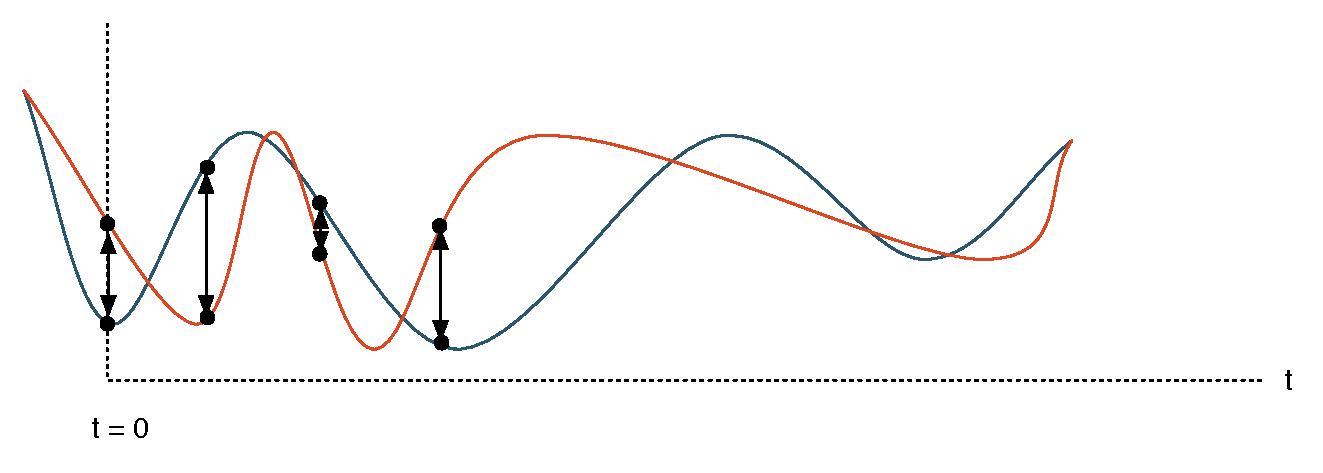
\includegraphics[scale=0.6]{TimbreDistance4}
\caption[Timbre Distance Between Time-Warped Curves]{An example of how a temporal warping of the exact same curve can result in non-negligible distance calculations between corresponding points in the resultant discrete sequences.}
\end{center}
\end{figure}
\\
DTW is a sequence similarity calculation method that attempts to align the time scales over which two different sequences of data occur by finding the optimal warping path between those time scales before calculating the distance over pairs of aligned points in the two sequences. For a more detailed overview and a real-time implementation of a close approximation, see (Salvador and Chan, 2004). We provide a diagram of the best warping path given the two sequences found in the previous figure in Figure 3.21. 
\begin{figure}[h!]
\begin{center}
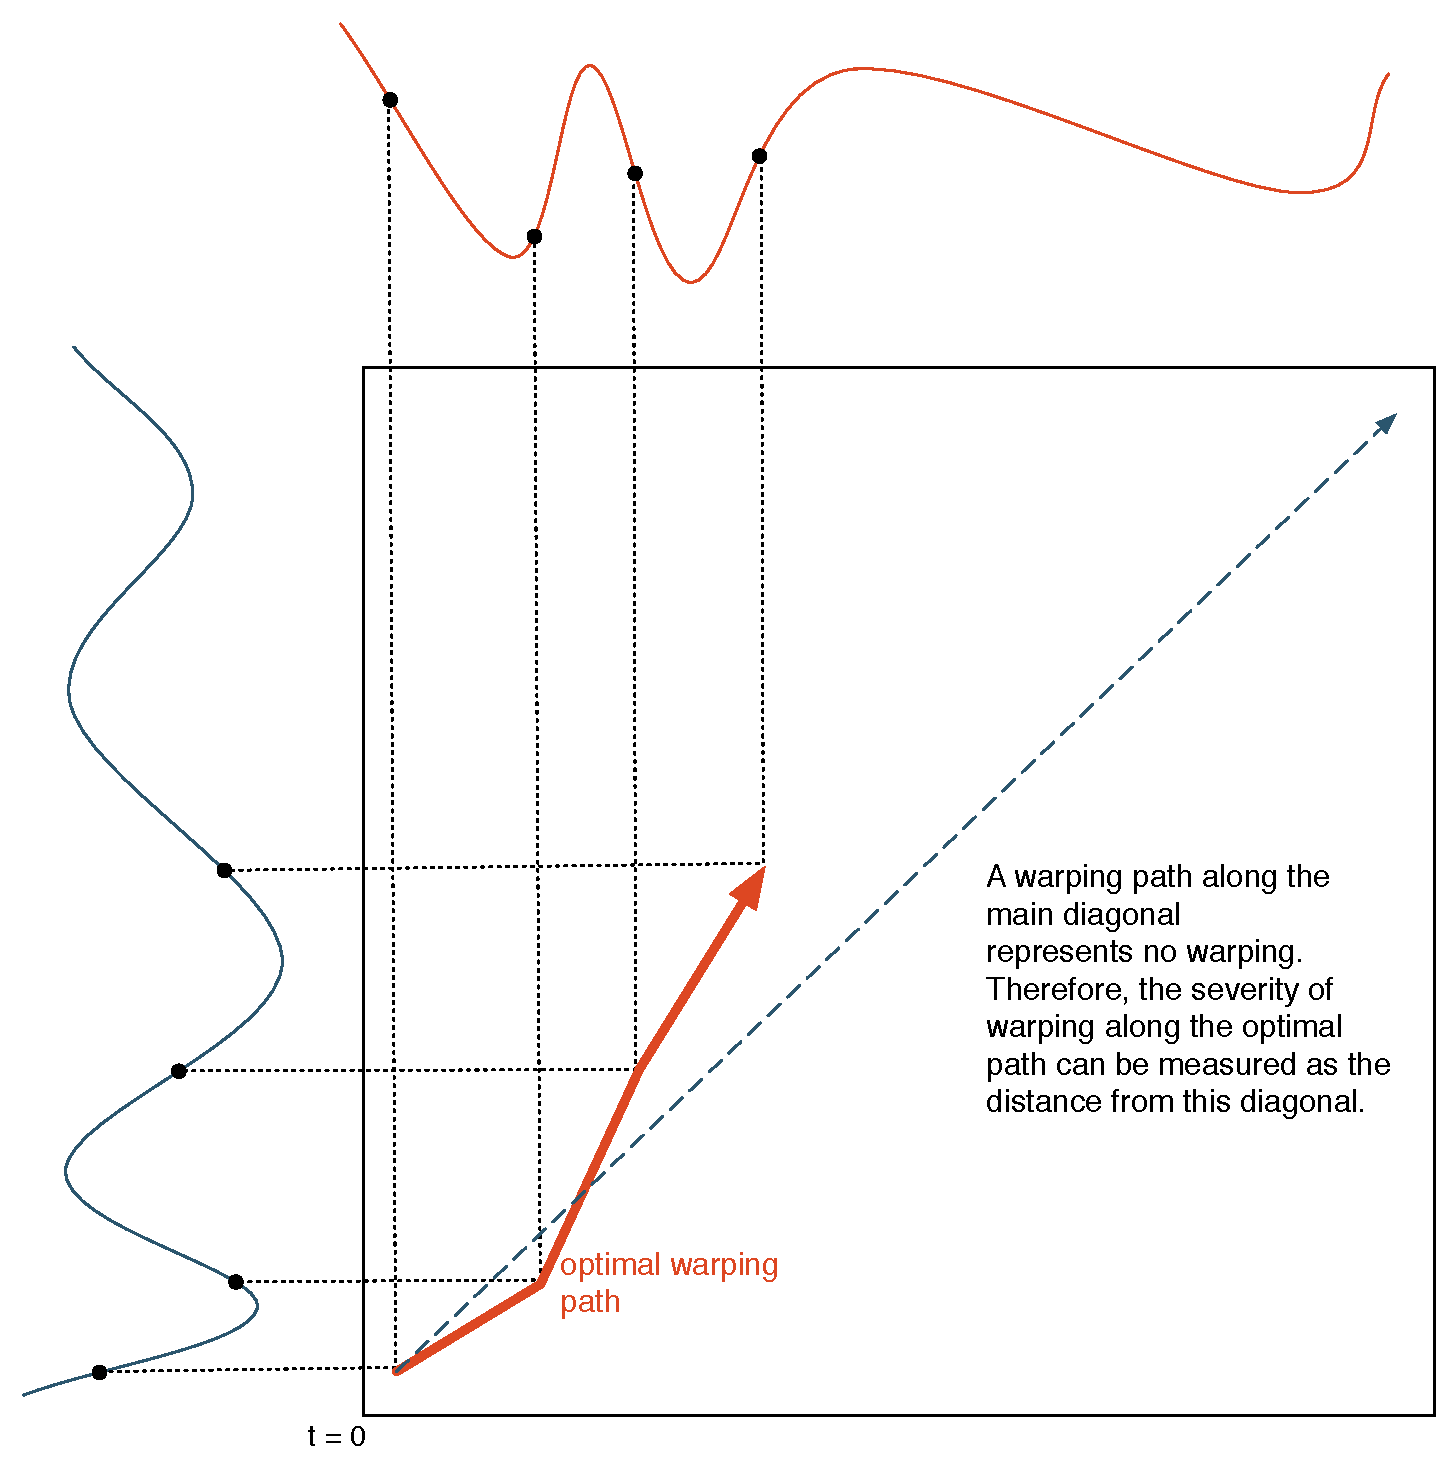
\includegraphics[scale=0.5]{DTWExample}
\caption[Timbre Distance Between Time-Warped Curves]{The optimal warping path between the two sequences from Figure 3.20 is shown.}
\end{center}
\end{figure}
\\
Note that given the optimal warping path, the sequences look identical (exemplified by the aligned points in the figure). Given the alignment this produces, accumulating distances between aligned pairs would result in a very small sequence distance and therefore a very high similarity.

DTW can be performed on sequences that have different lengths, which obviates the need for the same-length restriction required for the aligned-Euclidean measure. It is also important to note that if two timbre sequences are not time shifted or time warped, but instead could accurately be described using the aligned-Euclidean distance measure, DTW will most-often return a warping path that is near linear (i.e. very close to the main diagonal) so that the DTW result will match the aligned-Euclidean result. For this reason, the DTW measure can be seen as a more robust version of the aligned-Euclidean measure.

While DTW provides a metric that is invariant to time shifts and warpings and other temporal distortions (e.g. random sample deletion and random extension of static timbal content), there are situations in which it is not sufficient. The major drawback of DTW is that it requires that the beginning and ending of each sequence is aligned and that both sequences move forward in time from beginning to end. In other words, it can only search for the best global warping between two sequences. This is problematic given two sequences that are produced by the same object, but that contain a different amount of similar repeated subsequences. An example in our problem domain would be if we had two audio clips of the same bird chirping and breathing (labelled $A$ and $B$, respectively), with one clip containing three chirps followed by one breath ($AAAB$) and the other containing two chirps followed by one breath, followed by another two chirps ($AABAAB$). DTW would only search for paths that would align the two global sequences (likely resulting in a linear path through the first two $AA$s in each sequence and then stumbling to find an appropriate match to the third $A$ in the first sequence) and would fail to find an appropriate path to consider these two sequences similar, even though they in fact contain timbal subsequences that are almost exactly the same and that follow a similar sequencing of several $A$s followed by a $B$ (Serr\`a, G\'omen, Herrera, and Serra, 2008, p. 1143).

One solution is to eliminate the global alignment requirement of DTW. Serr\`a et al. propose a method they call Dynamic Programming Local Alignment (DPLA) that leverages both principles of DTW and the Smith-Waterman algorithm (a technique used in molecular biology that compares subsequences of all possible lengths to optimize a similarity measure) to find the longest similar subsequences from two sequences. DPLA uses only the data from those most-similar subsequences to calculate a similarity measure for purposes of cover song identification. In their problem domain, this measure works well because it is completely natural for cover songs to contain segments that are wholly different from the original and which therefore should be ignored as long as there is a long enough segment/subsequence that matches well with the original. In other words, an original song with structure $ABABC$ may have a cover with structure $BAADE$ (In this example, letters refer to subsequences of time-frequency patches that may or may not repeat within the overall sequence). Given the common occurence of such dramatic structural changes, these sequences should be considered similar and DPLA labels them as such. This is not an optimal similarity measure for timbre however, as a brief moment of a similar texture surrounded by vastly different sonic textures should not be considered to have an overall similar timbre evolution. While we do not want to enforce a global warping when comparing two timbre sequences, we do want a measure that takes the global sequences into account.

Given this, our approach extends DPLA to look for the best sequence of local subsequence alignments, where subsequences may be repeated, internally warped, and placed out of order, but such transformations are penalized. We have decided to penalize these transformations because we believe that too much of any will disrupt the overall sense of timbre. For example, a sequence of $ABCABC$ will be considered more similar to $AABCABC$ than $AAAABCABC$, more similar to $ABCABC$ where all subsequences are of the same length to those in the original $ABCABC$ than an $ABCABC$ where they are not, and more similar to $ABCABC$ than $CBABAC$.

An initial approach given the above could use a greedy algorithm that utilizes DPLA to find the longest common subsequence between sequences, removes those subsequences and repeats the process until an appropriate stopping criteria is met (e.g. the remaining sequence length after removing all paired subsequences is less than some threshold). However, the problem with this approach is that in certain cases a removed subsequence, $A$, may in fact be composed of two smaller subsequences, $B$ and $C$, one of which is repeated several times in one sequence and only once in the other. By removing $A$, $B$ and $C$ are also removed and therefore a repetition of $B$, for example, in one sequence would have no matching $B$ in the example with its only instance held within $A$ (see Figure 3.3.22).
\begin{figure}[!p]
\begin{center}
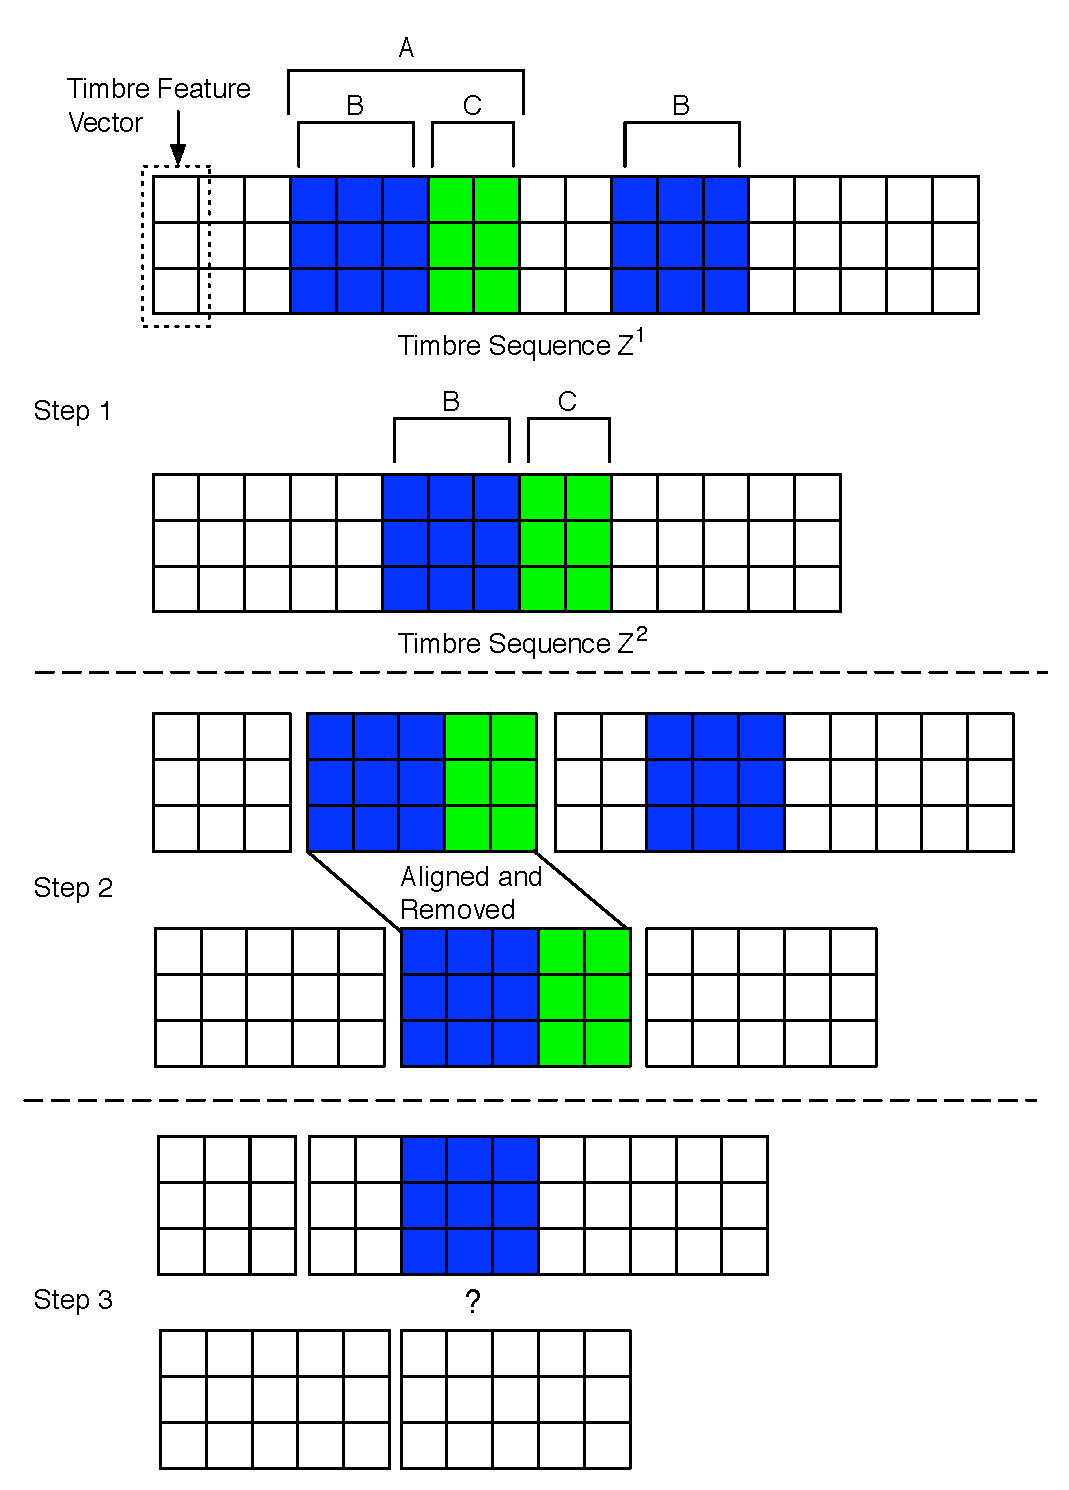
\includegraphics[scale=0.6]{GreedyMatching1}
\caption[Symmetric Greedy Removal After Matching]{In step 1, we search for the optimal local alignment between the two sequences. Once we find that alignment in step 2, we remove the subsequences involved from further consideration. In step 3, we have left a repetition of subsequence B stranded without a corresponding match in the second sequence.}
\end{center}
\end{figure}
\\
This issue arises because of the greediness of the approach. By removing a subsequence from contention from one sequence that the other could re-use to find an appropriate alignment to another one of its subsequences (e.g. $B$ in this example), we have weakened our ability to fairly find the best combination of optimal local alignments. We have given preferential treatment to one sequence (that which does not require an aligned repetition of $B$) over the other. This situation can occur over a single set of two sequences in both directions, so it isn't a matter of determining which sequence to prefer in our search if we use this greedy approach. 

A slightly less greedy option is to only eliminate the aligned subsequences of one sequence while allowing re-use of the entire other sequence throughout the alignment process. In other words, we start by finding the best subsequence alignment between two sequences $Z^1$ (the superior) and $Z^2$ (the inferior), remove that subsequence from $Z^1$ (but not from $Z^2$) and then search for the best local alignment between the two left over pieces of $Z^1$ and the entirety of $Z^2$, continuing along until all of $Z^1$ is aligned to some part of $Z^2$ (see Figure 3.23). 
\begin{figure}[h!]
\begin{center}
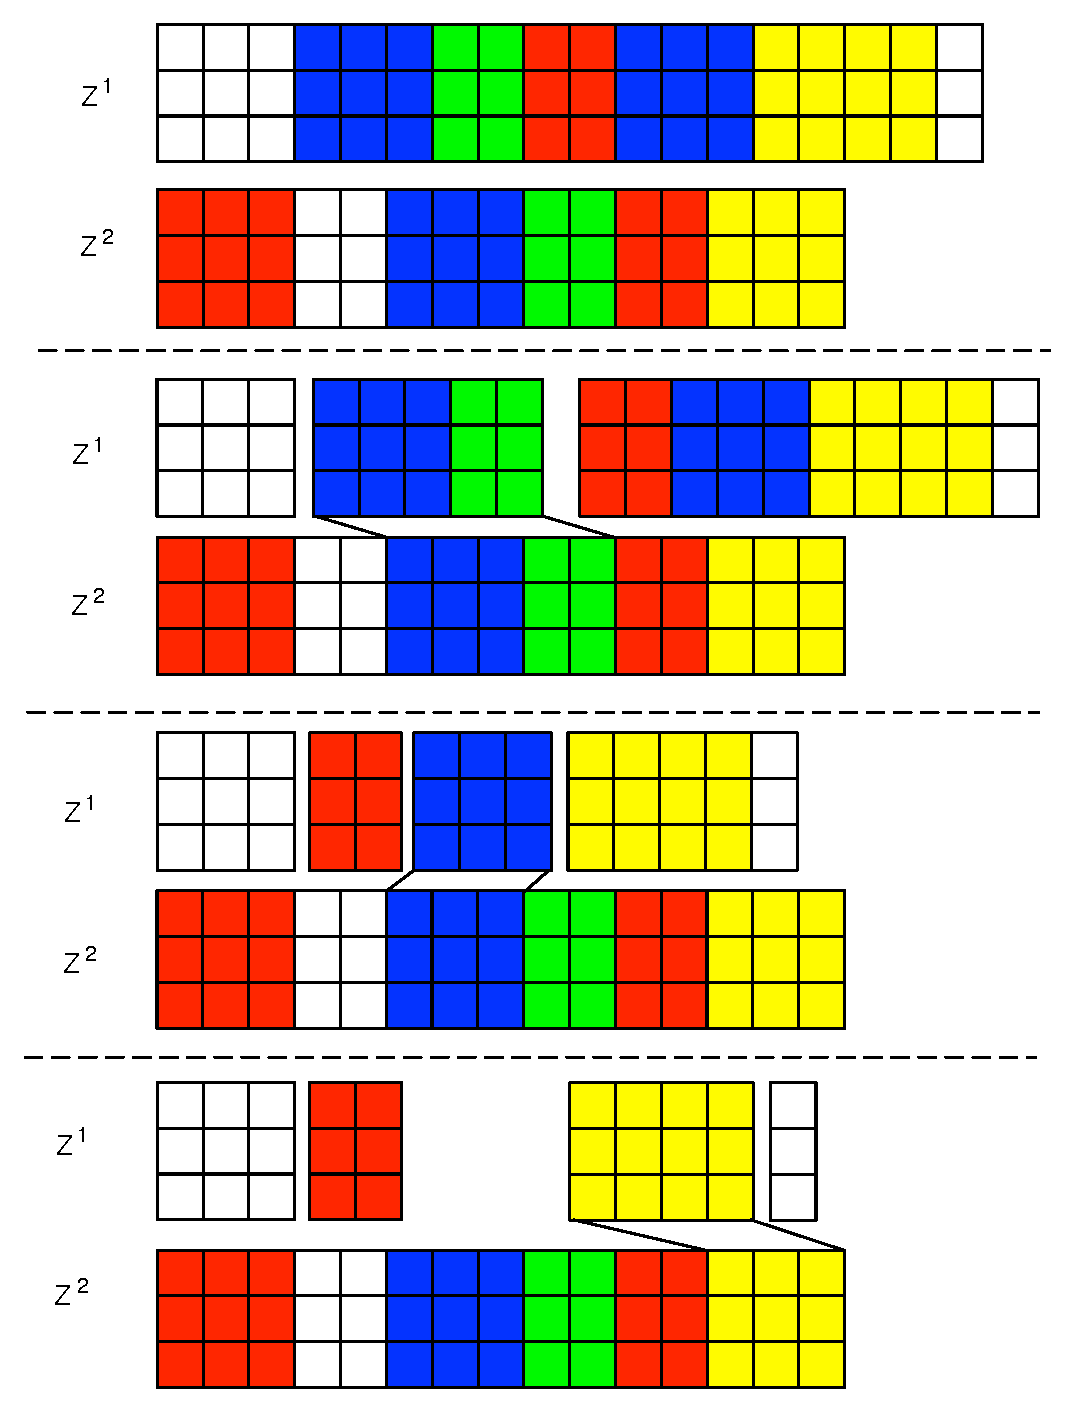
\includegraphics[scale=0.65]{GreedyMatching2}
\caption[Asymmetric Greedy Removal After Matching]{The optimally matched subsequences of $Z^1$ are removed after they are found, while $Z^2$ remains intact to provide $Z^1$ with the ability to match numerous subsequences to the overlapping content in $Z^2$}
\end{center}
\end{figure}
\\
This method obviously is biased towards finding appropriate matches in $Z^2$ to all of $Z^1$ (and not vice versa), but can be made symmetric by repeating the process in the opposite direction (removing aligned subsequences of $Z^2$ along the way, but reusing any aligned segments of $Z^1$) (see Figure 3.24). 
\begin{figure}[h!]
\begin{center}
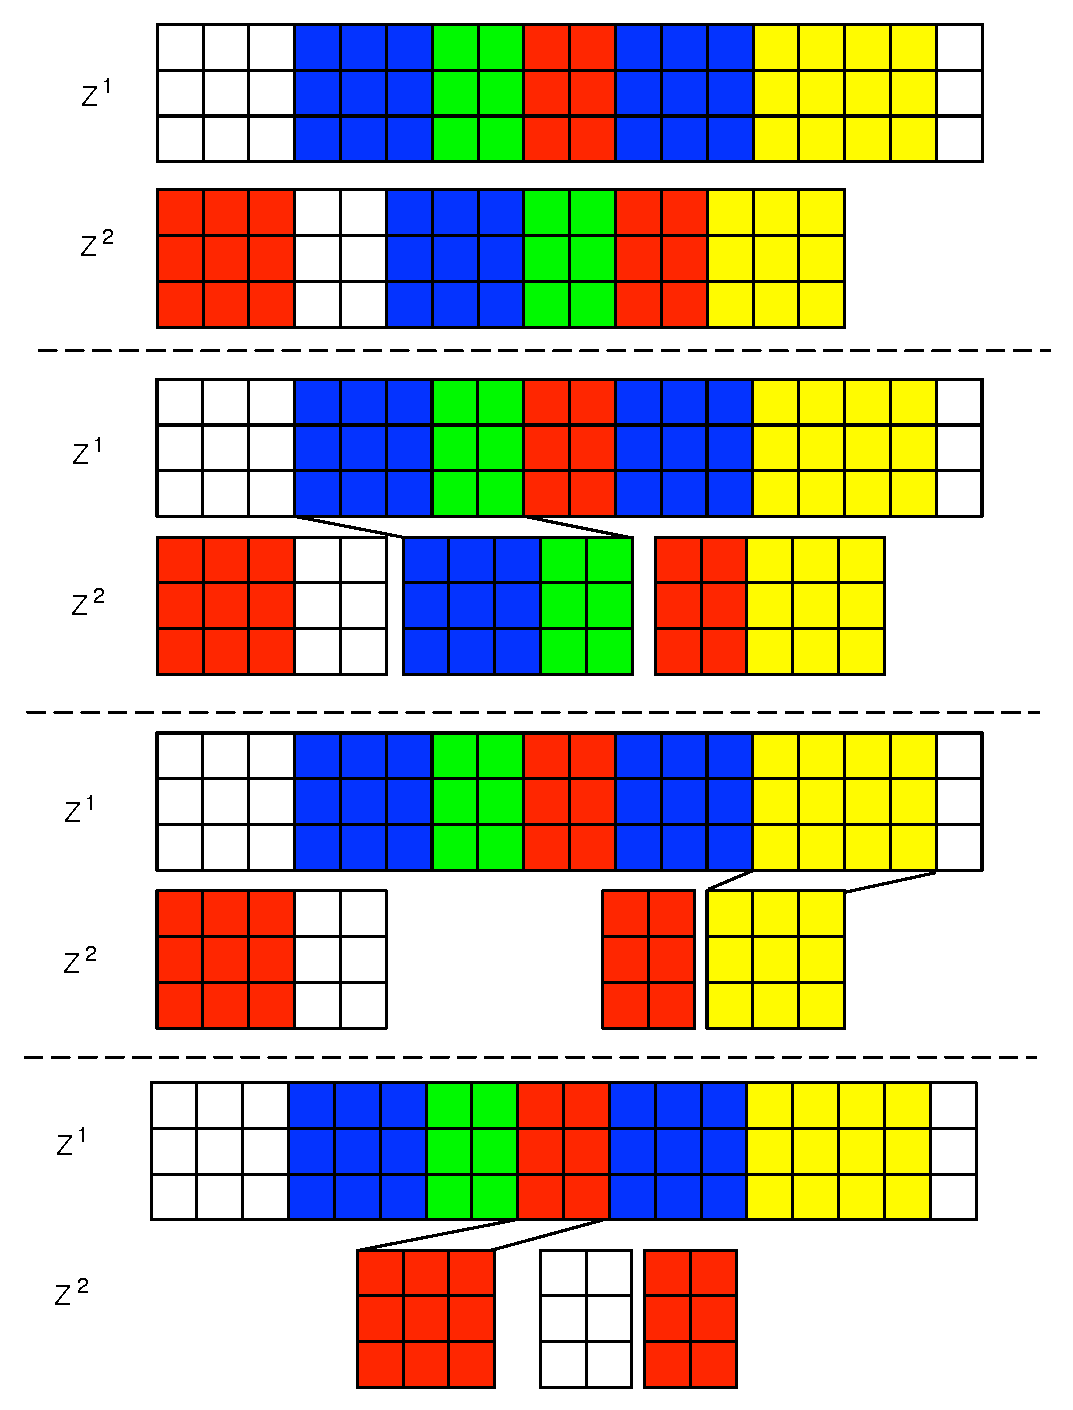
\includegraphics[scale=0.65]{GreedyMatching3}
\caption[Asymmetric Greedy Removal After Matching Reverse]{The optimally matched subsequences of $Z^2$ are removed after they are found, while $Z^1$ remains intact to provide $Z^2$ with the ability to match numerous subsequences to the overlapping content in $Z^1$}
\end{center}
\end{figure}
\\
The alignment combinations that are produced for each process can be used to calculate individual distance scores and then summed for a symmetric measure of similarity between both sequences:
\begin{equation}
S_T = \frac{2}{D_{SICSW}} \equiv \frac{2}{D_{ICSW_{1\to2}} + D_{ICSW_{2\to1}}}
\end{equation}
where $D_{SICSW}$ is what we call the Symmetric Iterative Continuous Smith-Waterman (SI-CSW) distance, $D_{ICSW_{1\to2}}$ is what we will call Iterative-CSW (I-CSW) distance calculated when treating $Z^1$ as the superior sequence (defined below) and $D_{ICSW_{2\to1}}$ is the I-CSW distance calculated when treating $Z^2$ as the superior sequence.

The remaining question is how one calculates the SI-CSW distance based on a number of subsequence alignments that may or may not be ordered appropriately in time, may or may not overlap in one or both sequences (this including repetitions), and may or may not include the entirety of both sequences. All of these must be considered in determining an asymmetric global sequence similarity score before averaging this measure over the results of the process in both directions. To begin, we must briefly overview the Smith-Waterman algorithm and discuss how we can leverage it for our problem domain.

As previously mentioned, DPLA utilizes the Smith-Waterman technique for performing local sequence alignment. This technique was first discussed towards finding ``maximally homogenous subsequences among sets of long sequences...in molecular sequence analysis.'' This problem domain differs from ours (as well as that of Serr\'a et al.) in that molecular sequences contain a fixed set of discrete values. This is an important distinction, because the Smith-Waterman technique typically is used in a problem domain where one will often find exact subsequence matches within a sequence. In its basic form, it takes a binary similarity matrix as its input based on this assumption, where one of the possible values represents `sameness' and the other, `difference.'

The way the Serr\'a et al. generate a binary similarity matrix between Harmonic Pitch Class Profile (HPCP) vectors - a standard, continuous-valued feature in the domain of cover song identification - is by using a thresholded similarity function with binary output (2008). If two HPCP vectors are similar enough, this threshold function considers them the same and if they are not, different. Serr\'a et al.'s ability to transform their problem into one that looks typical for Smith-Waterman allows them to use the technique `out of the box.' However, the goal of most problems utilizing the Smith-Waterman algorithm is slightly different from ours (in that we do not only consider exact matches between timbre vectors as being similar) and therefore we have decided not to try to transform our problem into one its standard implementation understands, but instead we have chosen to transform its standard implementation to one that fits our problem.

The Smith-Waterman algorithm assigns a positive value to two similar vectors and a negative value to two dissimilar vectors, so that ``these values have an average for long, random sequences...of zero.'' (Smith and Waterman, 1981, p. 196). This is important because we will be looking at the cumulative sum of these values over subsequences of vectors to determine whether they align well. If the cumulative sum is greater than $0$, we can assume this is not by chance and that these two subsequences should be aligned. In the standard implementation, pairs of vectors can only be labelled `similar' or `dissimilar' and therefore will only take on either a single positive value or a single negative value. By comparing all pairs of vectors in two sequences this way, one obtains a binary similarity matrix, $S$, where its elements $s_{ij}$ are positive if vector i from the first sequence and j from the second sequence are similar and a negative value if they are dissimilar.

However, the standard calculation of a binary similarity matrix is not required for Smith-Waterman to function appropriately. The important part of Smith-Waterman - and that which separates it from something like DTW - is that it creates inherent segmentation boundaries for optimally aligned subsequences due to its summation of both positive and negative similarity values. As already stated, the technique looks for subsequences who, over their length, accumulate positive similarity values (as will be discussed in detail below). Once these accumulations start to trend negatively, the alignments can be considered complete and local subsequence alignment boundaries are defined. Therefore, continuous valued similarity matrices may be used in Smith-Waterman as long as the elements can take both positive and negative values.

In our problem domain, we have already defined a similarity measure over individual timbre feature vectors that exist in our learned NLSE output space: Euclidean distance. We know this measure is appropriate because we specifically trained our pairwise CNN architecture using Euclidean distance as the cost function and tested the space's instrument clustering ability using a kNN classifier that utilized Euclidean distance as its metric. Therefore, we simply need to translate our Euclidean distance to a similarity measure that can take both negative and positive values in order to apply the Smith-Waterman algorithm. 

If we considered some boundary distance $\epsilon$ a distance from one timbre feature vector within which all other feature vectors are equally considered the same and outside of which all other feature vectors are considered different, we would be left with a binary similarity measure, which could be immediately input into the standard Smith-Waterman algorithm. However, this binary squashing operation is unnatural in that we want to be able to represent many gradations of timbre similarity and labeling all timbres within some radius of timbre space as equivalent does not allow this. Instead, we have chosen to linearly scale our distance measure into a range of $-1.0$ to $1.0$ so that the appropriateness of the Euclidean distance we learned is maintained in the measure. Our learned timbre space transformation takes time-frequency patches and reduces them down to points in 3-space within the cube enclosed by the range $[-1.0,1.0]$ in each of its three dimensions. Therefore, the maximum distance between two timbre points (i.e. the distance between two maximally dissimilar timbres) is $\sqrt{3*2^2} = 2\sqrt{3}$. This distance should correspond to a similarity score of $-1.0$ while the minimal distance between two timbre points (i.e. the distance between maximally similar timbres), $0$, should correspond to a similarity score of $1.0$. If all intermediate distances are linearly scaled between these two values we are left with the following similarity calculation between any two timbre vectors $Z_i^1$ and $Z_j^2$:
\begin{equation}
s(Z_i^1, Z_j^2) = 1.0-\frac{\sqrt{\sum_{k=1}^{N}(Z_{ik}^1 - Z_{jk}^2)^2}}{\sqrt{3}}
\end{equation}
If we apply this formula to all pairs of timbre feature vectors in the two sequences $Z^1$ and $Z^2$ and place the resultant $s(Z_i^1, Z_j^2)$ values into the elements $s_{ij}$ of a similarity matrix $S$, we can input this to the Smith-Waterman algorithm to find the best local subsequence alignment within the two sequences.

The Smith-Waterman algorithm builds an alignment matrix, often labelled $H$ (Smith and Waterman, 1981). We follow Serr\'a et al. in using a common variation of Smith-Waterman that applies `gap penalties' in constructing the alignment matrix, which allows for subsequence alignment even when there are small gaps or extensions in that alignment. These gap penalties are important in our problem domain, because we want to be tolerant of short insertions or deletions of timbal content in comparing the timbre similarity of two sequences, but this tolerance comes at a price (i.e. applies a penalty of allowance), so that it is limited during alignment. The alignment matrix elements can be calculated in the following manner (Serr\'a et al., 2008):
\begin{equation}
H_{ij} = max\left\{ 
  \begin{array}{l l}
    H_{i-1,j-1}+S_{i-1,j-1}-\delta(S_{i-2,j-2},S_{i-1,j-1})\\
    H_{i-1,j-1}+S_{i-1,j-1}-\delta(S_{i-3,j-2},S_{i-1,j-1})\\
    H_{i-1,j-1}+S_{i-1,j-1}-\delta(S_{i-2,j-3},S_{i-1,j-1})\\
    0
   \end{array} \right.
\end{equation}
\\
where:
\begin{equation}
\delta(a,b)=\left\{
  \begin{array}{l l}
    0 & \quad \text{if $b>0$}\\
    c_1 & \quad \text{if $b \leq 0$ and $a > b$}\\
    c_2 & \quad \text{if $b \leq 0$ and $a \leq b$}
   \end{array} \right.
\end{equation}
\\
\vspace{10 mm}
Note that $\delta(a,b)$ is $0$ when $S_{i-1,j-1}$ is positive. In the similarity matrix, this refers to the previous two vectors in our sequences being relatively similar, so that there is no gap in similarity. Therefore, no penalty is added. Gap openings and extensions result in two different penalty values ($c_1$ and $c_2$, respectively), so that we can vary those independently to penalize one over the other more. Serr\'a et al. found that their system evaluation measures were relatively constant when both $c_1$ and $c_2$ were between $0.3$ and $1.0$, so we will adopt their choices of $c_1 = 0.5$ and $c_2 = 0.7$. As a detail, note that the first three rows and columns of H cannot be calculated due to the gap penalty arguments and therefore are set to $0$.

In order to find the best local alignment within $H$, we simply:
\begin{enumerate}
\item Find the max value of all $H$ elements and trace back the alignment path to a $0$ (see Figure 3.25).
\begin{figure}[h!]
\begin{center}
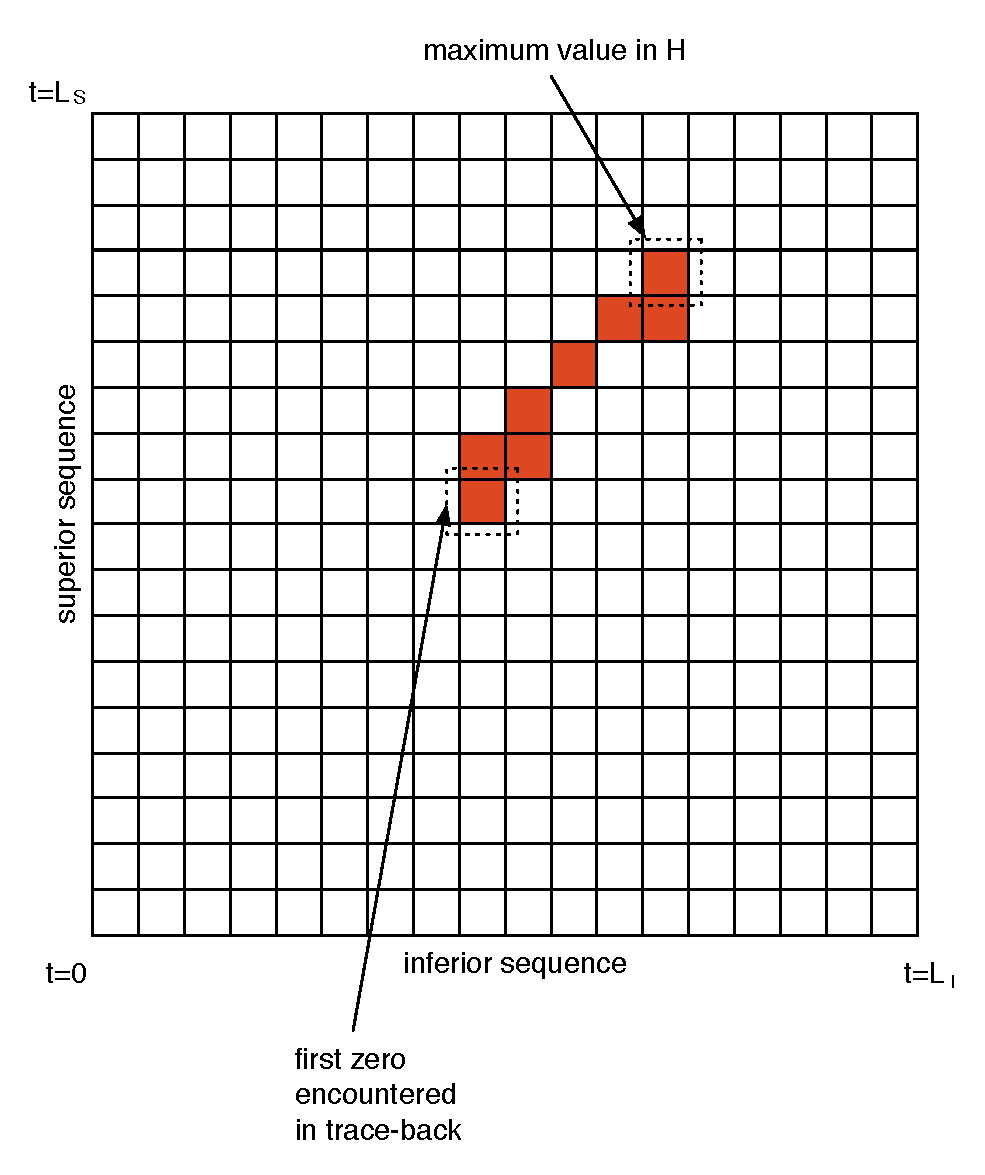
\includegraphics[scale=0.75]{SICSW_1}
\caption[Finding Optimal Subsequence]{The optimal local alignment ends with the maximum value of H. Once it has been found, we trace backwards (either below, to the left, or diagonally down and to the left) along the maximum values encountered until we find a $0$, which marks the beginning of the local alignment.}
\end{center}
\end{figure}
\\
\item Calculate the aligned-Euclidean distance over all aligned vectors found in step 1 and store this along with the length of the aligned vector sequences.
\end{enumerate}
This is where DPLA utilizing the Smith-Waterman algorithm ends, because it is only concerned with the best local alignment. As stated previously, we also are interested in this alignment, but we must continue to search for other subsequence alignments between what is left in our superior sequence and the entirety of our inferior sequence. Therefore, we continue on with the following steps:
\begin{enumerate}
\setcounter{enumi}{2}
\item Remove the submatrix from $H$ that corresponds to the superior sequence's subsequence used in the alignment found in step 1 and store this in H (see Figure 3.26).
\begin{figure}[h!]
\begin{center}
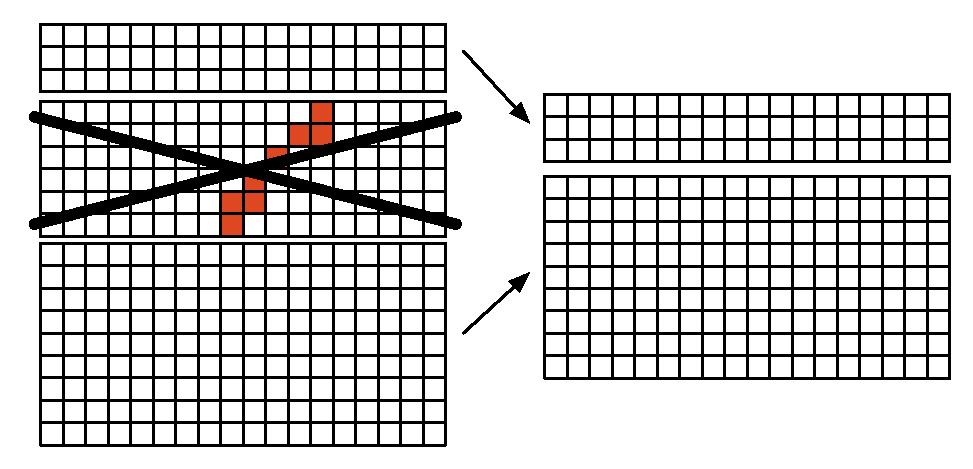
\includegraphics[scale=0.8]{SICSW_2}
\caption[Removing Optimal Subsequence]{After the aligned-Euclidean distance is calculated for the optimal local alignment, the superior's subsequence involved in that alignment is removed.}
\end{center}
\end{figure}
\\
\item Repeat steps $1-3$ until there are no longer any values in H above 0.
\item Calculate the sum of all distances generated in the various passes through step 2 and divide by the sequence length of the superior sequence to normalize for sequence length.
\end{enumerate}
This process will give us a preliminary value for the ${ICSW}$ distance in one direction (e.g. where $Z^1$ is treated as the superior sequence and $Z^2$ the inferior):
\begin{equation}
D_{ICSW_{S \to I}}^{(Prelim)} = \frac{\sum_{j=1}^J \sum_{k=1}^{K(j)} \sqrt{ \sum_{l=1}^L (A_{jkl}^1 - A_{jkl}^2)^2}}{L_S}
\end{equation}
where $D_{ICSW_{S \to I}}^{(Prelim)} $is the preliminary $ICSW$ distance from superior sequence $S$ to inferior sequence $I$, $J$ is the number of subsequences chosen for alignment, $K(j)$ is the length of the $j$th subsequence pair, $L$ is the dimensionality of our timbre vector, $A_{jkl}^1$ is the $l$th element of the $k$th vector in the $j$th aligned subsequence taken from $S$, $A_{jkl}^2$ is the $l$th element in the $k$th vector in the $j$th aligned subsequence taken from $I$, and $L_S$ is the length of $S$.

Once we calculate our preliminary I-CSW distances in both directions, we penalize the alignment combinations chosen by scaling the preliminary distances in the following ways:
\begin{itemize}
\item If alignments are not ordered appropriately in time (i.e. if the aligned subsequences do not progress forward in time for both sequences) then the appropriate I-CSW distance is scaled by the minimum number of subsequence swaps required to order the inferior sequence's segments plus the number of aligned subsequences, all divided by the number of aligned subsequences (see Figure 3.27). 
\begin{figure}[h!]
\begin{center}
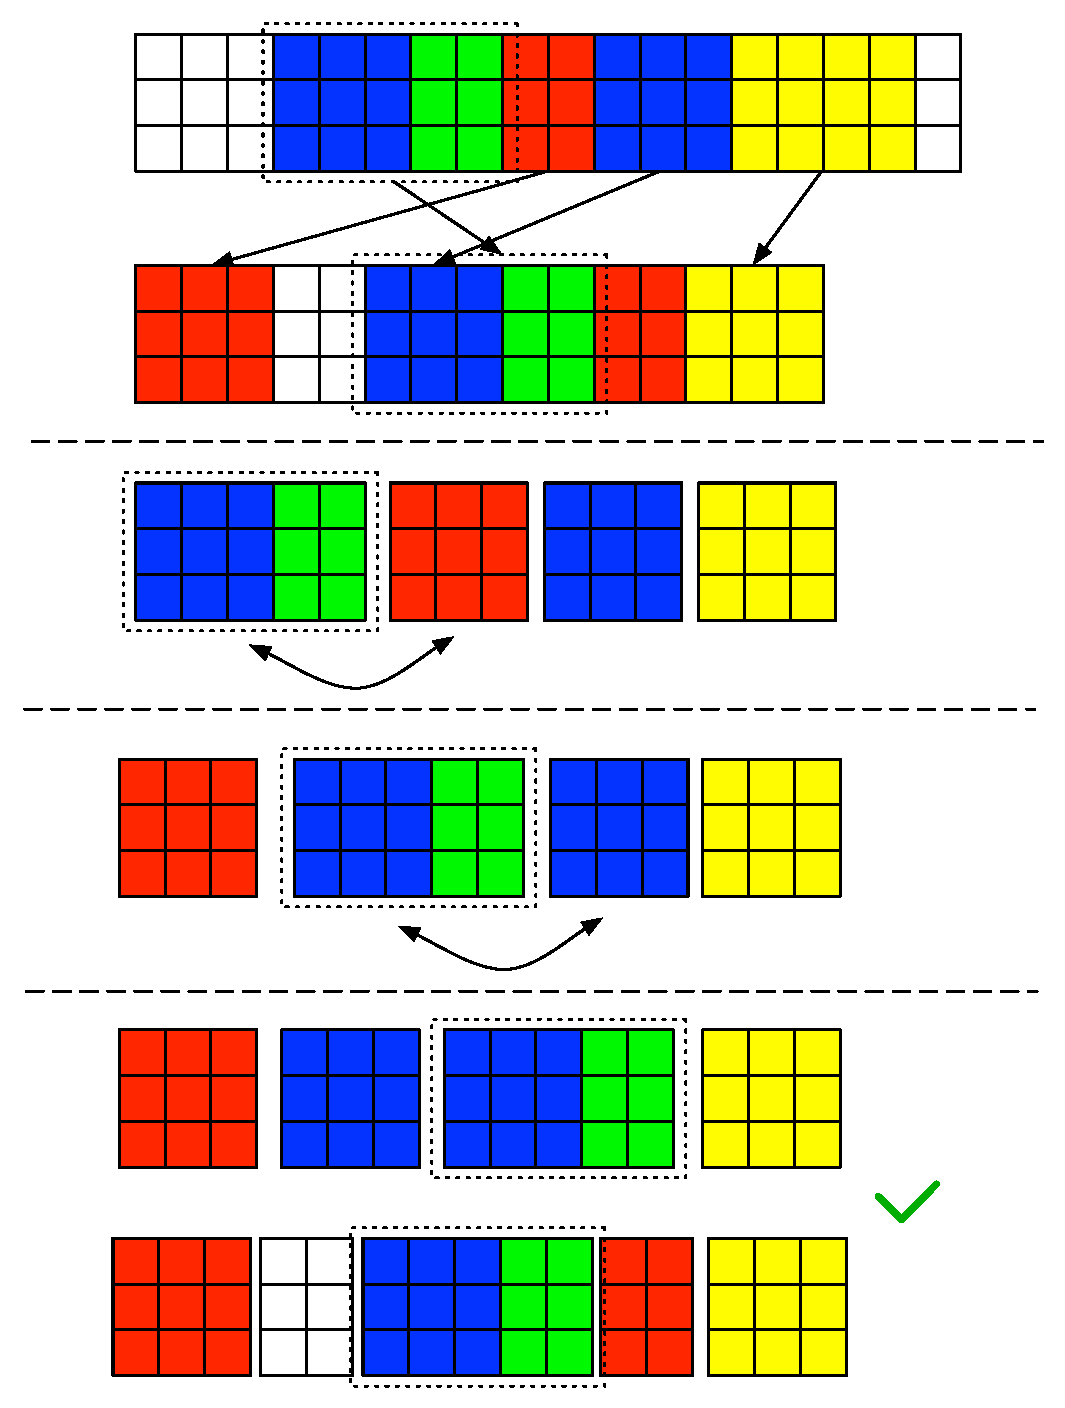
\includegraphics[scale=0.7]{Penalty_1}
\caption[Penalizing Swaps]{Two swaps are necessary to return the progression of aligned subsequences from the inferior sequence back to its original ordering.}
\end{center}
\end{figure}
\\
This value is therefore at least one (which occurs when the segments are appropriately aligned as they are). In other words, if the number of necessary subsequence swaps is $N_S$ and the total number of subsequences is $N_T$, the penalty multiplier will be:
\begin{equation}
P_{SWAP} = \frac{N_S+N_T}{N_T}
\end{equation}
\item Any overlap in the segments chosen from the inferior sequence are treated by determining whether their inclusion causes for more overlap than their exclusion causes for a gap between segments. If the overlapped segment causes for more overlap when included than gap when excluded, it is flagged as a `repetition' and dealt with separately (see next item). Once repetitions have been removed, the cumulative overlap and cumulative gap amounts are summed over the length of the entire sequence, added to the inferior sequence length, and then divided by the inferior sequence length, and this value is used to further scale the distance (see Figure 3.28). 
\begin{figure}[h!]
\begin{center}
\includegraphics[scale=0.7]{Penalty_2}
\caption[Penalizing Swaps]{The blue region is used twice by the superior sequence and is marked as a repetition, not to be penalized here. However, the two 2-vector gaps are penalized.}
\end{center}
\end{figure}
\\
This value is also at least one. If $L_O$ is the cumulative overlap, $L_G$ is the cumulative gap, and $L_I$ is the total length of the inferior sequence, the penalty multiplier will be:
\begin{equation}
P_{O/G} = \frac{L_O+L_G+L_I}{L_I}
\end{equation}
\item If any repetitions are extracted from the previous overlap/gap distance adjustment, they also affect the distance measurement, but to a lesser degree than an overlap, since repetition of a lengthy subsequence should not penalize the similarity of timbal evolution to a large degree. We penalize the distance measure by counting the number of repetitions, adding by the number of total subsequences extracted, and dividing by the number of subsequences extracted to give us a repetition adjustment scaling factor. If the number of repetitions is $N_R$, the penalty multiplier will be:
\begin{equation}
P_{REP} = \frac{N_R+N_T}{N_T}
\end{equation}
In the example in Figure 3.28 there is only one repetition of six total subsequences aligned, producing a $P_{REP}=(6+1)/6=7/6$.
\end{itemize}
The three scaling factors mentioned above are all used to adjust the preliminary I-CSW distances calculated in each direction (from sequence $Z^1$ to $Z^2$ and $Z^2$ to $Z^1$):
\begin{equation}
D_{ICSW_{S \to I}} = D_{ICSW_{S \to I}}^{(Prelim)} * P_{SWAP} * P_{O/G} * P_{REP}
\end{equation}

The two resultant I-CSW distances are then summed together to provide the SI-CSW distance ($D_{SICSW}$), which, as previously shown, is used to calculate our timbre sequence similarity measure, $S_T$.

It should be noted that our approach is still greedy in that we optimize local alignments without regard to how it will affect our overall global scores (i.e. we optimize before applying our scaling factors), but we believe it to be a considerable upgrade over typical DTW and non-time warped aligned-Euclidean methods. A more systematic and less greedy measure is left for future work.

In order to test our approach versus the three approaches discussed above (aligned-Euclidean, global DTW, and DPLA), we developed a controlled experiment that starts with a sound and applies various kinds of temporal distortion that should not alter its timbal similarity score. The distortions applied are broken into the following categories:
\begin{itemize}
\item Slight global time scaling (randomly selected between $2-5\%$) combined with time shifting (randomly selected between $100-500ms$).
\item Local time warping (randomly selected such that the warping path does not diverge from the diagonal more than 5 frames).
\item Random sample deletion (randomly selected and totalling between $2-5\%$ of all content).
\item Random extension of stable timbral content randomly selected and totalling between $2-5\%$ of all content. 
\end{itemize}
We measure how invariant each model is to these temporal distortions by considering a nonzero distance between the original sample and one of its distorted versions as an error. We measure these errors given a number of different sample files and average over each distortion.

We then progressively distort our target in way that produces sounds that we would like to consider less and less timbrally similar by:
\begin{itemize}
\item Introducing new timbal content (between $10-50\%$ of the file length) while randomly deleting other content.
\item Re-ordering random subsequences within content (by choosing subsequences that are between $10-20\%$ of the file length and swapping out of order up to 5 times).
\item Randomly inserting repetitions paired with random deleting of non-repetitive segments (by choosing subsequences that are between $10-20\%$ of the file length and repeating up to 3 times).
\item Applying severe temporal warpings (randomly selected such that the warping path diverges at least more than 10 frames once during the length of the file). 
\end{itemize}
In these cases, we want the amount of distortion severity to be inversely proportional to the similarity calculated. We therefore measure how the similarity calculated changes as a function of increased distortion severity. For example, we look at the rate at which the similarity measure decreases as the introduction of new timbal content increases from $10-50\%$ of the file length.

\subsection{Genetic Operator Variations}
In order to implement a genetic algorithm within an automatic programming framework, one needs to develop an appropriate representation of each program, which we have done in section 3.1.2. This representation allows us to represent all programs as a set of trees. However, this is not enough to define an input space. In order for a set to become a space, a topological ordering must be placed on the elements. This ordering will inform the shape of the objective landscape (i.e. fitness function) and therefore directly influence the difficulty of search through the space for some desired solution. In algorithm space, such orderings are typically not made explicit due to its complexity. Instead, implicit orderings are acquired via the operators used to search the space (da Silva, 2008, p. 102). Thus, using different operators will result in different input-space orderings. The goal is to find the input-space ordering that makes the objective landscape as �searchable� as possible. This can be measured via the negative slope coefficient (NSC), developed by Vanneschi (2004, p. 54).

The NSC is computed by first generating a fitness cloud, where one plots the fitness of an individual by the fitness of one of its neighbors (children in GP parlance). The shape of this cloud provides some intuition of the evolvability of the genetic operators used and thus some intuition about the difficulty of the problem using these operators (Vanneschi, 2004, p. 130). It is important to note that Vanneschi found that uniform random sampling of individuals to use in the generation of the fitness cloud typically results in generating individuals whose fitnesses tend towards the lower end of the fitness range and therefore does not give a complete picture of how fit neighbors are for individuals throughout the entire fitness spectrum (2004, p. 132). Instead, Vanneschi suggests using the `Metropolis-Hastings' sampling technique, which have adopted in our work. For pseudo-code explaining the technique see (Vanneschi, 2004, p. 131).

Vanneschi also notes that choosing an appropriate neighbor from an individual (via that application of a genetic operation) is only useful if that neighbor would not be immediately discarded via the selection mechanism. Therefore, Vanneschi suggests that neighbors are found via a Tournament Selection (see Section 3.2.5) process that we also have adopted, where $k$ randomly generated neighbors enter a tournament and the winner is chosen as the neighbor to use in the fitness cloud. Following Vanneschi's suggestion, we will choose only one neighbor per individual, which will be selected as the winner of a tournament of size $k=10$.

The NSC is calculated by partitioning the x-coordinate of the scatterplot into M segments of the same length and then dividing the y-coordinate into the ranges spanned by each x-segment. The average x and y values are calculated in those regions and a piecewise linear function is generated through those points. The slopes of the piecewise segments are calculated and only the negative values are summed to provide the NSC. In other words, for each segment $S_i$, the slope $P_i$ is calculated in the following way:
\begin{equation}
P_i = \frac{N_{i+1}-N_i}{M_{i+1}-M_i}
\end{equation}
where $M_i$ is the average of the original individuals' fitness values within the $i$th partition and $N_i$ is the average of the selected neighbors' fitness values within the $i$th partition. The NSC is calculated from these slopes as:
\begin{equation}
NSC = \sum_{i=1}^{M-1} max(0, P_i)
\end{equation}
If $NSC = 0$, the problem is considered easy, if $NSC < 0$ it is difficult, and the value of NSC quantifies this difficulty (p. 139). In our experiments, we have chosen $M=10$ so that we can generate enough points per segment of the fitness cloud given a relatively small sample size of $1000$ for the average values to be descriptive of the segment.
The genetic operations we have decided to test are the most common set found in GP problems. A brief description of each follows:
\begin{description}
\item [Crossover] - In crossover, two trees are selected at random within the population, a subtree from each is selected and removed, and then the subtrees are attached to the cut points of the opposite trees. When ensuring syntactic correctness through the search process, the crossover operation must make sure to only choose subtrees that can be swapped and still result in syntactically correct structures (see Figure 3.29). 
\begin{figure}[h!]
\begin{center}
\includegraphics[scale=0.5]{Crossover}
\caption{Tree crossover with the root (i.e. dac\texttildelow{} below the terminals).}
\end{center}
\end{figure}
\\
\item[Subtree Mutation] - This, unlike Crossover, is a unary operator, which removes a subtree at a random location within a tree and replaces it with a randomly generated subtree. As with crossover, syntactic rules must be enforced during generation of this new subtree (see Figure 3.30).
\begin{figure}[h!]
\begin{center}
\includegraphics[scale=0.5]{SubtreeMutation}
\caption{Subtree mutation with the root (i.e. dac\texttildelow{} below the terminals).}
\end{center}
\end{figure}
\\
\item[Point or Node Replacement Mutation] - Instead of removing an entire subtree and replacing it with a randomly generated subtree, Point Mutation randomly removes a single node in a tree and replaces it with a node that is syntactically valid in that position (i.e. with the same number of inputs and the same input/output types) (see Figure 3.31).
\begin{figure}[h!]
\begin{center}
\includegraphics[scale=0.5]{PointMutation}
\caption{Point mutation with the root (i.e. dac\texttildelow{} below the terminals).}
\end{center}
\end{figure}
\\
\item[Reproduction] - This is the simplest of all genetic operators in that it is simply a pass-through mechanism for selected patches. Reproduction allows for highly fit individuals to remain in the population from generation to generation so that they may be involved in crossover with other individuals (and so they can be continuously mutated) in the hope that a higher fit individual will result (see Figure 3.32).
\begin{figure}[h!]
\begin{center}
\includegraphics[scale=0.5]{Reproduction}
\caption{Reproduction with the root (i.e. dac\texttildelow{} below the terminals).}
\end{center}
\end{figure}
\\
\end{description}

We have decided to use the following combinations of genetic operators (and proportions of how many patches undergo each operation in the combination) and have tested their ability to simplify the search problem using NSC:

\begin{itemize}
\item 75\% Crossover, 25\% Subtree Mutation
\item 75\% Crossover, 25\% Point Mutation
\item 25\% Crossover, 75\% Subtree Mutation
\item 50\% Crossover, 25\% Subtree Mutation, 25\% Point Mutation
\item 50\% Crossover, 25\% Subtree Mutation, 25\% Reproduction
\item 25\% Crossover, 50\% Subtree Mutation, 25\% Reproduction
\end{itemize}
As previously mentioned, each of these tests will consist of generating $1000$ patches using the Metrpolis-Hastings sampling technique and selecting one neighbor for each of these patches from the winner of a Tournament Selection process involving $10$ randomly generated neighbors in a manner consistent with the combinations listed above.
\subsection{Target Sound Selection}

The previous discussion has provided a means to develop an appropriate fitness function for our problem and an input space that makes its corresponding fitness surface (given the pre-defined fitness function) as easily-searchable as possible within the GP framework. Going forward, we want to make sure that what we are testing is the appropriateness of our search technique over this space and corresponding fitness surface and not the appropriateness of or ability for sounds to to actually be realized in Max. For example, there may be time-varying timbres that require tens of thousands of Max objects to replicate perfectly.

As Mitchell and Creasey point out in their work on sound matching via evolutionary methods, the difficulties in obtaining an optimal solution to a complex search problem are based on several factors, only one of which is the search algorithm itself (2007, p. 1). They recommended using a `contrived' target in order to test only the efficacy of the search. In our problem domain, a contrived target refers to one that was generated by a known synthesizer (i.e. Max patch). Mitchell and Creasey suggest randomly generating contrived targets using points uniformly spread out in the input-space (p. 2). If the search algorithm is able to match all of the contrived targets with a good spread in the input space, it is suggested that one can then assume it will be able to match any target (p. 2). This assumes however that a uniformly spread set of points in the input space will map to a large area of the timbre space, which is not necessarily the case.

We therefore have chosen to test the search algorithm on three contrived targets with varying degrees of complexity in order to attain an understanding of the limitations of the search algorithm (see Figure 3.33). Since these contrived targets are realizable in the Max environment, they should be found given an intelligent enough search. While it is important that these targets are sufficiently spread out in the input space in order to promote some sense of generalization of the search technique through this space, we later test the search technique using non-contrived targets in order to provide a more resounding argument for this (as is discussed in 3.2.7).

We are able to measure success in two different ways when using contrived targets and will speak to both in the results section whenever our tests involve them:
\begin{enumerate}
\item We are able to compare the topographies of the contrived-target patch and the best-of-run patch that is generated during the search process. If the topographies are exact matches, we must consider this an outright success. However, if different, the topologies provide intuition about how code bloat enters the search, how well the topologies of local optima mirror the target topology (i.e. if there is a correlation between timbre and topology space), and how well different topologies can mimic the timbre produced by a contrived-target topology (i.e. how realizable is the target timbre given topologies that differ from the topology that generated the target).
\item We are able to measure the best-of-run fitness and determine how well our search is able to achieve its goal of finding a patch that can produce the target timbre.
\end{enumerate}

\subsection{Limiting Code Bloat and Promoting Parsimony}

By using contrived targets and objects that are able to construct them perfectly, we have set up a self-fulfilling prophecy of sorts that would rarely be encountered in practice. It is important to look at how our solutions degrade (or the time it takes to find an optimal solution increases) once the object set grows beyond the necessary set of objects and/or necessary objects are removed from the object set. However, before these parameters are varied, we look at other sorts of resource limitations that have proven effective in other GP research to see if they are useful in this problem space. We are able to focus on the efficacy of these methods and provide appropriate comparisons if we tightly control our experiments in the way suggested.

In the Prior Work section, we listed a number of methods for limiting the region of input space we search including: Enforcing strong typing constraints, applying either static (SMTD) or dynamic maximum tree depths (DMTD), and/or enforcing limitations on the total amount of resources in a given population using either resource limited GP (RLGP) or dynamic resource limited GP (dRLGP) constraints. These methods were developed to be used for any problem domain and only discriminate against solutions that are not parsimonious or syntactically valid. They promote efficiency and low storage requirements as well as controllability of the resulting algorithms due to their propensity to generate low-dimensional parameter sets. However, as with any kind of limitation of the searchable input space, we must make sure not to exclude possible solutions. Therefore, a fine balance must be found between the improvements in the efficiency of the search (i.e. iteration count to the optimal solution) and the decrease in fitness of the optimal solution found. Since we can be sure that all solutions are attainable for our contrived targets and associated object sets, we can fairly compare different severities of limitation across all targets.

A brief recount of each limitation follows:

\begin{description}
\item [Static Maximum Tree Depth (SMTD)] - Throughout the entire search process, a static limit is placed on the maximum tree depth of each individual's representation.
\item [Dynamic Maximum Tree Depth (DMTD)] - Throughout the search process, the limit placed on the maximum tree depth is increased in order to slowly evolve more and more sophisticated (i.e. complex) algorithms.
\item [Resource Limited GP (RLGP)] - Throughout the entire search process, a static limit is placed on the number of resources (i.e. the sum of function and terminal nodes) used in an entire population. This limit is therefore applied to the overall population as opposed to SMTD and DMTD, which is applied to each individual in a population.
\item [Dynamic Resource Limited GP (dRLGP)] - Throughout the search process, the limit placed on the amount of resources available to a population increases in order to slowly evolve more and more sophisticated algorithms.
\end{description}

To test the effects of these limitations, we use the contrived target set, apply these limitations at various severities, and calculate both how error increases (i.e. how fitness decreases) as a function of the amount of limitation as well as how quickly solutions can be found as a function of the amount of limitation. This analysis provides us with an optimal degree of limitation that balances both an increase in efficiency with a decrease in accuracy.

Since we have not yet discussed nor tested how best to initialize our population, nor how we should select individuals to undergo genetic operations to produce each successive generation, we choose to use the most common methods for these tests, Grow Initialization and Fitness-proportionate Selection (see Section 3.2.5), and improve upon these (if improvements are possible) in separate testing. On each permutation of the aforementioned limitation, we are interested in recording the fitness of the best-of-run individual, the iteration/generation in which that individual was created, the total number of iterations in each run, and the trends of average fitness of each generation, maximum fitness in each generation, and minimum fitness in each generation, so that we can analyze how quickly solutions are found, how good they are, and whether or not the various trends mentioned seem to level off by the time the last generation is assessed. In our testing, we run tests while imposing each of the following search space limitation constraints over $200$ iterations of $100$ individuals, for each of the contrived targets:
\begin{itemize}
\item A SMTD of $4,5,6,7, \text{and }8$.
\item A DMTD between $4-6$, $6-8$, and $4-8$ with the limit increasing at equal steps along the $200$ iterations.
\item A RLGP of $1000, 2000, 3000, 4000, \text{and } 5000$.
\item A dRLGP between $1000-3000$, $2000-4000$, and $1000-5000$ with the limit ramping up linearly over the $200$ iterations.
\item A SMTD of $5$ and a RLGP of $2000$ and SMTD of $8$ and a RLGP of $5000$.
\item A DMTD between $6-8$ and a dRLGP of $2000-4000$ and DMTD of $4-8$ and a dRLGP of $1000-5000$.
\end{itemize}

\subsection{Initial Conditions and Selection Methods}

Along with algorithm representation and operator selection, the population initialization and selection mechanisms form the basis of the GP architecture. It may seem strange to first look at limiting code bloat and promoting parsimony before exploring these fundamental GP mechanisms. We have chosen this ordering because of the benefits reducing code bloat and promoting parsimony provides to all testing that follows it. Testing of the remaining parts of our system requires full test runs. By applying the mechanisms explored in the previous section, these test runs will be able to run more efficiently by not looking in regions of the input space that we are not interested in (i.e. those that would produce syntactically invalid Max patches or those whose solutions would be complex and likely unable to run in Max in real time, which is a desirable properly of any synthesis algorithm).

The three initialization flavors we study are Full, Grow, and Ramped Half-and-Half initialization. A brief description of each of these methods follows:
\begin{description}
\item [Full Initialization] - The root node is chosen and then, in a depth-first fashion, function nodes are added until the maximum tree depth is reached, at which time a terminal node is chosen. This process is repeated for all branches, resulting in a full tree where each branch meets the maximum tree depth. The risk of using full initialization is that one may start with a population where individuals are too similar (given that they are all full tree structures).
\item [Grow Initialization] - This is very similar to Full initialization, except that as the branches are being built, each node is selected from the pool of both function and terminal nodes. The result is a tree with branches that are no greater than the maximum tree depth, but that may be shorter (due to a terminal node being chosen before the maximum depth is reached). The risk of using Grow initialization is that it may result in a population with too many individuals that have terminated prematurely and are therefore too simple to perform any meaningful function.
\item [Ramped Half-and-Half Initialization] - This is the most common form of initialization in Genetic Programming. It uses Full initialization for half of the individuals in the population and Grow initialization for the other half. It also increases the depth limit for both methods as the population grows in size. The ramping of the depth limit along with using both Full and Grow methods produces a wide variety of patches in shape and size.
\end{description}

The four selection methods we have chosen are known as Fitness-Proportionate, Ranking, Tournament, and Double Tournament. A brief description of each of these methods follows:
\begin{description}
\item [Fitness-Proportionate Selection] - Individuals from one generation are chosen to populate the next generation with probability proportional to their fitness. Thus, the more fit an individual is, the more likely it will be chosen to breed new individuals for the next generation. In figure 34, the top row of squares represent the individuals in a population and the pie chart below represents their respective fitnesses as fractions of the sum of all fitnesses in the population. In other words, for fitness-proportionate selection, the pie chart illustrates the probability with which each individual will be selected to breed the next population. Note in the figure that the red and green individuals from this example are chosen twice due to their high fitnesses (i.e. probabilities of selection), while the yellow is not chosen due to its low fitness.
\begin{figure}[h!]
\begin{center}
\includegraphics[scale = 0.7]{PieChartSelection}
\caption{Fitness-proportionate selection}
\end{center}
\end{figure}
\\
\item [Ranking Selection] - In ranking selection, individuals from one generation are ranked in order from least to most fit and the probability of selection is proportional to this ranking. For example, if there are $N$ individuals in a generation, then the least fit individual has rank $1$ and the most fit rank $N$. The sum of all ranks is $N*(N+1)/2$. Therefore, least fit individual will have a selection probability of $1/(N*(N+1)/2)$ or $2/(N*(N+1))$ regardless of its fitness value and the most fit individual will have a selection probability of $N/(N*(N+1)/2)$ regardless of its fitness value. 
\item [Tournament Selection] - In tournament selection, a set of patches are selected at random from a generation and the most fit of those patches is selected. All patches are placed back in the pool of all patches to be randomly sampled from on the next iteration. This random sampling of patches and the tournament that follows is repeated as many times as there are individuals to be selected.
\item [Double Tournament Selection] - In Double Tournament selection, each individual chosen to be part of a tournament is already the winner of a tournament with different conditions. The most common Double Tournament Selection mechanism works by first choosing a random grouping of patches, selecting the most parsimonious of those patches with probability $D$, and placing the winner in a pool of other parsimony tournament winners to be involved in a fitness tournament. The idea is that Double Tournament Selection applies parsimony pressure absent from typical Tournament Selection, which is useful for controlling code bloat. The most common tournament size for the parsimony tournament is two with $D = 0.7$ and the most common tournament size for the fitness tournament is seven (Luke \& Panait, 2006, p. 21).
\end{description}

We have chosen to enumerate the various combinations of initialization and selection mechanisms as it is unclear exactly how correlated these two mechanisms are in producing an optimal search algorithm. We are interested in determining how the best-of-run average fitness error over all contrived targets varies as we test these combinations as well as how they affect the resultant algorithm complexity (measured as the size of the topology of the best-of-run patch). Therefore, for each tested combination of initialization mechanism and selection mechanism, we record these values and compare. Again, our tests will involve moving through $200$ iterations of $100$ individuals. The combinations we test are listed below:
\begin{itemize}
\item Full initialization and Fitness-Proportionate Selection.
\item Full Initialization and Ranking Selection.
\item Full Initialization and Tournament Selection.
\item Full Initialization and Double Tournament Selection.
\item Grow Initialization and Fitness-Proportionate Selection.
\item Grow Initialization and Ranking Selection.
\item Grow Initialization and Tournament Selection.
\item Grow Initialization and Double Tournament Selection.
\item Ramped Half-and-Half Initialization and Fitness-Proportionate Selection.
\item Ramped Half-and-Half Initialization and Ranking Selection.
\item Ramped Half-and-Half Initialization and Tournament Selection.
\item Ramped Half-and-Half Initialization and Double Tournament Selection.
\end{itemize}
We aim to strike a balance between algorithm complexity and fitness so as to provide the user with a controllable architecture (i.e. one with a small number of variable inputs) and therefore choose an initialization/selection mechanism combination that allows us the best trade-off. This selection along with the choices made given the aforementioned tests will provide us with an optimal base GP architecture. The following tests seek to augment this architecture and provide further evidence that it will generalize well to all timbres.

\subsubsection{Non-standard Selection Methods}

Aside for the above methods of patch selection for the subjection to genetic operations, we referred to three other non-standard flavors of mechanisms involved in the selection process in the Prior Work section that have shown to be useful for certain GP problems:

\begin{enumerate}
\item Using the \textbf{Parallel and Distributed Genetic Programming (PADGP)} paradigm, where subpopulations within the GP population are formed and individuals between populations are rarely allowed to interact, such that the subpopulations are allowed to evolve independently. The parameters to this model are the communication topology between subpopulations (i.e. whom transfers individuals to whom), the number of subpopulations, the number of individuals per subpopulation, the frequency of exchange of individuals, and the number of individuals exchanged (Vanneschi, 2004, p. 178). The three communication topologies used in the literature are the ring topology (where the subpopulations form a circle and each passes individuals in a clockwise manner), the grid topology, (where subpopulations form a grid and each population sends and receives individuals from all four neighbors), and the random topology (where each subpopulation sends individuals and receives individuals from exactly one random subpopulation different from itself at each migration period).
\item Applying \textbf{Simulated Annealing (SA)} on the parameter set of each patch in a population to find the optimal parameter set for the given patch topology before running the patches through the selection process.  
\item Starting with a more lenient fitness function that the selection mechanism is aware of and making it more demanding over the lifecycle of the search, such that only in the last few iterations is the appropriate fitness measure applied before selection. The set of fitness functions involved are formally referred to as \textbf{Increasingly Discriminating Fitness functions (IFFs)}. 
\end{enumerate}

We believe our treatment of this problem would not be complete if we did not ascertain whether these more modern GP mechanisms could be helpful to us. The above approaches attempt to provide a more efficient means to achieve an optimal solution and we therefore test them on this ability. We calculate statistics on how quickly (i.e. how few iterations) we are able to perform in order to find a near optimal solution. In the case of using SA in combination with GP, it is not immediately clear how to directly compare this strategy with standard GP, due to the internal iterations SA proceeds through within each GP iteration. In this case, the number of algorithms searched (i.e. translated into the Max environment for audio processing) will be used for a fair comparison.

In our testing involving PADGP, we follow Venneschi's suggestion to use a random communication topology, a frequency of exchange of every ten generations, and a population exchange size of $10\%$ of the total number of individuals in each subpopulation (Vanneschi, 2004, 190). We test this method using $200$ iterations of $100$ individuals, where the $100$ individuals are split into $5$ groups of $20$.

In testing Simulated Annealing on the parameter set of each patch in a population between generations, we limit the system to search through as many individuals as we are in a typical run (i.e. $20,000$). If we allow each patch to undergo $10$ SA iterations, this reduces the number of iterations of GP to $20$. We do not want to limit the ability of our system to utilize GP and we feel that $20$ is possibly just enough iterations to leverage it, so we keep the SA iteration count at $10$. SA is a simple strategy that generates a random neighbor, calculates its fitness and a corresponding `acceptance probability' given that fitness and the fitness of the current individual, compares the probability to a uniformly randomly chosen number, and makes the neighbor the new individual to run SA on if the probability is greater than the random number chosen. As the iteration count increases, the acceptance probability becomes more and more strict for poorly performing individuals. As is standard, we will use the Metropolis-Hastings algorithm to choose neighbors (where a neighbor in this context is a patch with the same exact topology, but where a single parameter is changed by no more than $50\%$ of its magnitude) and will assume an acceptance probability of:
\begin{equation}
P(S_{T_{p_1}}, S_{T_{p_2}}, T) = \left\{
   \begin{array}{l l}
    1 & \quad \text{if $S_{T_{p_2}}>S_{T_{p_1}}$}\\
    e^{-(S_{T_{p_2}} - S_{T_{p_1}})/T} & \quad \text{if $S_{T_{p_2}}\leq S_{T_{p_1}}$}
    \end{array} \right.
\end{equation}
where $S_{T_{p_1}}$ and $S_{T_{p_2}}$ are the similarity scores for some patches $p_1$ and $p_2$, and $T$ is the `temperature value', which will range from $1-10$ over the ten iterations (Kirkpatrick, Gelatt, and Vecchi, 1983, p. 673).

We also test the use of Increasingly Discriminating Fitness functions (IFFs) as the system iterates through its search process. We choose to alter our discrimination by applying a warping to the similarity function used to generate the similarity matrix input to our CSW implementation. Recall that this function takes the following form:
\begin{equation}
s(Z_i^1, Z_j^2) = 1.0-\frac{\sqrt{\sum_{k=1}^{N}(Z_{ik}^1 - Z_{jk}^2)^2}}{\sqrt{3}}
\end{equation}
where the similarity is calculated between any two vectors in the sequences $Z^1$ and $Z^2$ being compared.

\subsection{Expanding/Restricting the Searchable Region of Input Space}

After the controlled experiments from above - meant to compare variations of each GP mechanism against one another - have been performed, it is appropriate to move away from the perfectly contrived examples we have used so far. Stepping away from these tests towards a `real-world' scenario involves two steps:

\begin{enumerate}
\item We will both expand and contract the object and parameter (by discretizing with greater and less resolution) sets used to generate Max patches when searching for our contrived targets. By looking at how well (or how quickly) our solutions approach the contrived Max patches, we will be able to show how robust our system is to starting with an inappropriate resource set (i.e. one with objects that are not involved in the optimal solution and/or with necessary objects in the optimal solution not present). Even if the system is given a timbre that was produced (or is easily producible) by a Max patch, it is likely any object set we choose for our system to source from will not contain all of the objects (and only the objects) necessary to build the target. Since a `real-world' timbre may not even be realizable with 100\% percent accuracy in the Max environment, these tests are not enough to show how well our system will generalize to all timbres. However, they are a good first step towards that goal and provide us with more information (namely, the patch topologies of both the target and the solution to compare) to use to assess the robustness described.
\item The final step towards showing system generalization over all timbres involves using timbres that are not contrived. This is discussed in the next section (3.2.7 Generalization).
\end{enumerate}

In order to test how well our system performs given object and parameter sets that are either not sufficient or over-complete, we look at how well our performance drops off as we restrict or expand our object and parameter sets over our contrived examples. We have chosen to use the following sets for each example in our tests:

The important data we gather from tests include how the best-or-run patches' fitnesses decrease as we change the cardinality of the function set away from only containing necessary functions and as we change the possible parameter values that functions may take, as well as recording how the iteration count required to reach a best-of-run patch varies given changes in these variables.

\subsection{Generalization}
It is necessary to test this system on a number of real-world sounds in order to gauge its ability to generalize to sounds that are not contrived. As Riionheimo and Valimaki note, ``the quality of resynthesis of real recordings is more difficult to measure as there are no known correct parameter values'' nor synthesis topologies (2003, p. 13). In genetic programming research where a known target algorithm does not exist, the performance of the system is usually measured using the fitness level at which the system converges and how long it takes to converge to that level. We do not have a known topology for such real-world examples and therefore must only use this measure to determine how successful our search method is. In order to determine how well our search generalizes over all real-world sounds, we have chosen five different target sounds ranging from those generated by music instruments to those generated in nature. A brief description of the timbres we have chosen follows:
\begin{itemize}
\item
\item
\item
\item
\item
\end{itemize}
We have searched for these timbres using the optimal parameters/methods obtained in the previous tests, varying a stopping criteria based on iteration count - with runs ending at $200$, $400$, $600$, and $800$ iterations - and a fitness threshold (which is based on the results of the timbre similarity tests). We have calculated the typical statistics (min, max, mean) over each stopping criteria variation for each individual target as well as all targets combined. The results of these tests can be found at the end of \textbf{Chapter 4 - Results} with an accompanying discussion.

\newpage
\nocite{*}	% This says to cite all refs in the bib file
\bibliographystyle{apacite}	% apa style
\bibliography{mybib.bib}		% name of bib file
\end{flushleft}
\end{document}